\section{What Would be Activities Called Research?}
\label{chapter-what-is-research}

「研究の定義は何か?」よりも、「私たちは研究をどのように特徴づけたらいいのか?」とかの方がいいかも?

To create an agent capable of conducting research autonomously, it is crucial to understand what research is in the first place. Therefore, in this section, I would like to discuss the characteristics of what is called research. Particularly, I will strive to discuss a definition that can encompass activities called research, regardless of differences in fields such as humanities, natural sciences, and mathematics.



However, please note that my aim here is not to identify the universally acceptable ``true'' definition of research, which is beyond my ability. Rather, I will endeavor to describe various characteristics of research to  provide a starting point for engineers and researchers who aim for realizing research-capable AI. Therefore, the definition of research that I'm going to discuss in the following sections is merely an operational definition. I hope that further discussions among researchers will deepen towards a better definition of research.

\subsection{Research as Knowledge Production}

正当化の目的が真理促進的であることを書いたら、for society はいらない気がする?認識である以上主体は必要だというのは間違いない。全部書いてみて後で検討。

研究による成果には、偽であるが真であるように見える命題がある。なので、知識の生産というよりも、知識の候補を生み出しその確からしさについての確証を強めていくという方が適切かもしれない。偽であった時にも有用な情報。なので、知識を生み出すというよりも、知識を生み出すことを試みるとした方がいいかも。

\textcolor{red}{
知識を生み出すではなく、知識を生み出すことを目指す・試みる、とする。なぜなら命題は必ずしも真ではないし、偽であると適切に判定されることは有用な情報をもたらすから。そう考えると、「この世界の未知の真理を明らかにしようとすることが研究」という方が適切????←知識の中に「真である」ということが含まれているのと、正当化に真理促進性を要求してるので、どちらでも変わらない気がする?知識を生み出そうとするだと生み出せなかった時が単に失敗という感じになってしまう?違うな。検証が命題Aを肯定すると、Aという知識が生まれるが、命題Aを否定すると、Aの否定という知識が生まれるというだけの話。なので問題なし。なので、「知識を生み出すことを試みる行為」でいい気がする。
}

\textcolor{red}{
既存の定義に触れる
}

A widely accepted definition of research would be that research is the attempt of generating new knowledge. It seems that research, regardless of the field, requires some novelty, and it feels reasonable to say that research is an act of creating knowledge based on past knowledge. Thus, I will tentatively adopt this definition as the working definition in this paper. 

\textcolor{red}{
In particular, I will consider that research is the production of new knowledge for society. I included ``for society'' because knowledge appears to be relative to society, as I will discuss later. 
}

% For instance, in physics, a new explanation for a phenomenon is produced, in mathematics, a new proof for a theorem is presented, and in engineering, a new design blueprint for creating something is generated, all as new knowledge.

% \begin{figure}[htb]
%     \centering
%     
\includegraphics[width=0.8\linewidth]{figs/reseach_definition.pdf}
%     \caption{Definition of Research}
%     \label{fig:definition}
% \end{figure}

% \subsubsection{Some Notes on Research and Science}

% The reason why I deliberately use the word ``research'' instead of ``science'' is because I want to include fields like engineering, humanities and arts, which are not typically referred to as science, within the scope of automation in the long run. Science refers to a methodology for generating knowledge, and I believe that new knowledge is not necessarily produced only by scientific methods. I believe that so-called humanities and arts also share some commonality of producing new knowledge. Therefore, the definition of generating new knowledge can be said to encompass these fields as well.

% Of course I admit that science is the most rigorous and reliable framework for knowledge production. Because of its power and popularity, most of the existing analysis on research is about science. My discussion would also be centered around the discussion of science, though I try to present the view not limited to science. 

\textcolor{red}{
論文の目的をもっと先に明確に書くことで、こういうただし書き的なのを減らす。
Please note again that this definition is provisional. By viewing research as the production of knowledge, we can indeed characterize the wide range of current human research activities comprehensively, which is why I adopted this definition. However, as we will see later, in attempting to create a comprehensive definition, it can result in aspects that seem counterintuitive to characterize certain research. It's possible that aiming for a definition that is not field-specific is not desirable (i.e., striving for the realization of an intelligence capable of such a task is not desirable), and it might be better to seek a definition with a more narrowed scope of application. I will revisit and discuss how research should be defined at the end of this section.
}

\subsection{Knowledge Production as Belief Revision}
\label{section-knowledge-production-as-belief-revision}
I have defined research as the generation of new knowledge. Then, what exactly is knowledge, and what does it mean to produce knowledge? I will explore this question in this section. 

Defining knowledge and knowledge production rigorously is a philosophical debate that has not yet been settled \cite{sep-epistemology}, and I won't delve into it deeply here. Instead, I would like to provide some primitive ideas that can serve as a starting point for further discussions on how to realize an artificial researcher.

\subsubsection{Knowledge as Belief}
The question of what is the thing called knowledge has been a subject of debate for a long time in the field of \textit{epistemology}, which is one of the branches of philosophy. So, for now, I would like to refer to the discussion in this field as an example and see how research can be characterized if I do so.

In epistemology, knowledge had been classically considered to be \textit{justified true belief (JTB)} \cite{sep-epistemology}. The term ``true'' is difficult to define rigorously, but for the purpose of discussion, let's think of it as something being fact. ``Belief'' can be provisionally understood as someone's thought or conviction about something. And ``justified'' means that it is deemed reasonable to hold such a belief. What justification means has been discussed in epistemology as a central point of contention. Since the criticism that JTB is not appropriate as the definition of knowledge \cite{gettier1963justified}, how to modify or expand JTB to make it a suitable definition of knowledge has seem to be a major discussion in epistemology \cite{sep-epistemology}. 

While most philosophers don't seem to believe that these properties are sufficient to define knowledge, there seems to be some agreement that they may be necessary \cite{sep-epistemology}. Even in the epistemology discussion, it seems that rather than abandoning the JTB altogether, the discussion seemed to center on how to expand upon it, using the JTB as a base. Therefore, let me tentatively assume that knowledge is JTB in this paper as a starting point for the discussion. In the following section, I will examine how research is perceived as an activity when adopting this definition. Examining the discrepancy and alignments between the consequences of this examination and what we expect from a research-capable AI will provide seeds of thought for a better definition of research and hence what that AI should be able to do.

\subsubsection{Knowledge Production as Belief Update}
The purpose of research can be said to be revealing the unknown truths of this world. Therefore, the justification in research is demanded to be such that it determines propositions as true if they are true, and false if they are false. Such justification is called truth-conducive. There are various discussions about what justification is, but it can be said that justification in research should be truth-conducive.

Therefore, producing knowledge could be said to be constructing a new proposition that refers to this world and determining its truth or falsity through such justification. If knowledge is regarded as belief, this can be rephrased as holding the belief that a proposition is true and updating this belief through truth-conducive justification.

% Furthermore, as I will discuss later, we justify the belief that a certain hypothesis is true or false in an extremely robust and sound way that would convinces everyone. Given such justification, it seems not so problematic to depict research through the subjective concept of belief in a substantial sense.


% 知るということは、私たちに対してこの世界とその真実があり、私たちがその真実を認識するということです。すなわち、知るという概念はあくまで私たちと世界との両方の存在を前提としている概念であり、その意味で知る主体に依存する概念です。知識の定義に信念という主観的な概念が出てくるのはこのためです。したがって、知識が信念であるとは直感に反するように思われるかもしれませんが、この意味で妥当であるように思われます。

% 知識が信念であるというのは、知る/知っているという概念がそれを知る主体に依存する概念だからです。私たちの外側に世界があり、その中のある真実を私たちが認識するというのがこの定義の意味での知るという行為であり、それはあくまでも世界とそれを認識する主体との関係性を前提として成り立つ概念です。


% It may feel counterintuitive to hear that knowledge is belief. However, there is a reason for this. It is because the concept of ``knowing'' depends on the subject.

% It may feel counterintuitive to hear that knowledge is belief and research is the updating of belief. However, I think that perceiving the production of knowledge as the updating of beliefs is not so unreasonable. This is because, for example, the validation of a hypothesis by an experiment can be interpreted as a strengthening of the belief that the hypothesis is true. Specially in science, we become more convinced of its validity as a hypothesis survives repeated various verifications. This research practice appears to be well aligned with the view of research as a renewal of beliefs.

\subsection{Knowing Depends on Knowing Subjects}

% \subsubsection{知るということと主体の存在の関係}
To know means we recognizing the truths of this world. In other words, the concept of knowing fundamentally presupposes the existence not only the known object but also the knowing subject. This is why the definition of knowledge involves the subjective concept of belief. Therefore, while the idea that knowledge is belief may seem counterintuitive, it appears valid in this sense. Particularly, since justification in research should be truth-conducive, the knowledge produced would be objective. In this sense, using belief, which is a subjective concept, to define research does not seem to be much of a problem.

Moreover, viewing research as the updating of beliefs does not seem too far removed from the practice of research itself. For example, the validation of a hypothesis by an experiment can be interpreted as a strengthening of the belief that the hypothesis is true. Specially in science, we become more convinced of its validity as a hypothesis survives repeated various verifications. This research practice appears to be well aligned with the view of research as a renewal of beliefs.


\subsubsection{Knowledge for Humans}
As mentioned earlier, research is an endeavor aimed at revealing the unknown truths of this world, and the knowledge generated there must be novel. Then, what does it mean for knowledge to be new or unknown?

Knowledge was a justified belief about whether a certain hypothesis is true or false. Therefore, unknown knowledge could be a state where such a belief is not held at all, or even if it is held, it is not justified. I believe that this is what ``unknown'' means.

Since the concept of knowing depends on the knowing subject, naturally, the concept of the unknown is also subject-dependent. In research, we do not consider knowledge unknown just because a single individual is unaware of it. It is only when none of us know it that we consider it truly unknown. That is, it seems that the knowledge we create through research is required to be knowledge for all of humanity. This is why the definition adopted this time includes ``for society''.


% 前述したように、研究はこの世界の未知の真理を明らかにすることを目指す営みであり、そこで生み出される知識は新規である必要があります。それではある知識が新しい、あるいは未知であるとはどういう状態でしょうか。

% 知識がある仮説が真である/偽であるという正当化された信念でした。であるならば、未知の知識とは、そのような信念がそもそも抱かれていない、あるいは信念が抱かれていてもそれが正当化されていない、状態だということができるでしょう。

% 知るという概念は知る主体に依存した概念でしたので、当然未知という概念も主体に依存した概念です。研究においては誰か一人の個人が知らないだけではその知識が未知であるとみなしません。我々の誰一人としてそれを知らない時に初めて未知であると考えます。すなわち、私たちが研究で生み出す知識は、人類全体の知識であることを要求されているように思われます。これが今回採用する定義に for society を加えた理由です。


% No matter how rigorously you produce knowledge, if it is already known, it cannot be called research. Therefore, we have defined research as the process of producing ``new'' knowledge. In this section, I will briefly discuss what would it mean for knowledge to be unknown or novel.

% It seems that something being unknown to someone can be described as a state where the person has attempted to know something, but the answer is not present in their mind. Therefore, it can be said that when knowledge born from research of a question is considered new, it refers to a situation where there has been no hypothesis that everyone believes to be sufficiently plausible for the question.\footnote{
% While presenting a question that no one has posed ensures that the knowledge is new. Even in such cases, no one also yet knows which hypothesis is correct for that question. This is why I have mentioned only about the unkownness of hypotheses
% }
% In other words, once knowledge is considered as belief, being unknown seems to be interchangeable with having a low level of confidence, which sounds a bit counterintuitive. In this sense, it seems appropriate to say that research transforms a hypothesis with low confidence into one with higher confidence, rather than turning the unknown suddenly into the known.\footnote{
% Here, saying ``there has been no hypothesis that everyone believes to be sufficiently plausible'' is merely to imply nuances that knowledge is belief and that a hypothesis is never fully proven to be true. You can just read it as ``there is no answer'' for simplicity.
% }



% As mentioned later, research can be described as the act of posing questions, proposing hypotheses in response to them, and then verifying those hypotheses to update beliefs on whether the hypotheses are correct. Therefore, it can be said that when knowledge born from research of a question is considered new, it refers to a situation where there has been no hypothesis that everyone believes to be sufficiently plausible for the question\footnote{
% While presenting a question that no one has posed ensures that the knowledge is new. Even in such cases, no one also yet knows which hypothesis is correct for that question. This is why I have mentioned only about the unkownness of hypotheses
% }. For example, we do not know how to create a general-purpose artificial intelligence, which can be said to mean that we do not have an answer (a hypothesis with high confidence) to the question, ``How do you create a general-purpose artificial intelligence?''.

% I said in the paragraph above that ``research is the process of transforming the unknown into the known.'' However research can also be seen as the updating of beliefs, as I have explained. Therefore, the binary depiction of an object suddenly transitioning from the states of unknown to known does not seem appropriate. Rather, it seems more reasonable to consider that beliefs continuously change and I just call some group of belief states unknown and others known, for convenience.

% I don't know precisely what it means to be unknown. This is a difficult problem, but let's consider it naively. 
% I consider a knowledge to be unknown when for a question a subject lacks any hypothesis which he/she has a JTB that the hypothesis is true. For example, I do not have the answer to the question of ``How to realize an artif icial general intelligence.'' So the knowledge of ``the way to realize an artificial general ingelligence'' is unknown. \textcolor{red}{TODO: Add explanation}

% In research, a single verification does not always immediately turn a hypothesis into true or false. Rather, hypotheses that withstand repeated verifications through various experiments by different researchers gradually come to be regarded as more plausible. Therefore, it seems to me appropriate to say that research transforms a hypothesis with low confidence into one with higher confidence, rather than turning the unknown suddenly into the known. In that sense, it seems somewhat justified to describe new knowledge as something for which there wasn't a highly confident hypothesis before.

% The expression ``unknown'' could be more appropriately expressed as ``high degree of unknownness''. Because knowledge production is a continuous concept of belief updating, therefore, unknownness is also a continuous concept. In reality, there are multiple hypotheses with varying degrees of certainty concerning a particular question. The state of knowledge being unknown can be expressed as not having any hypothesis among these hypotheses with a particularly strong level of justified certainty.

% First, research begins with a particular question. The state of not knowing the answer to this question is what I consider the state of being unknown. In other words, it can be thought of as a state where I don't know what the candidate hypotheses, which are the potential answers, are like, or a state where I know the candidate hypotheses but don't know their plausibility. These are states where I have not been able to find hypotheses or sets of hypotheses that can be assigned a particularly high degree of confidence from the set of potential answers to a given question. Therefore, provisionally and casually, it might be said that the state of ``not having highly confident beliefs (or a set of beliefs) for a particular question'' is unknown, and the state of having highly confident justified beliefs is known.

% Of course, there are issues with this clarification. For example, it is unlikely that I can select a single highly confident hypothesis from the entire set of possible hypotheses. Also, rather than feeling equally confident about all possible hypotheses, it seems that I implicitly distinguish between hypotheses that seem relevant and those that do not. Furthermore, it is unclear to what extent I consider a state to be unknown based on the degree of confidence. However, these are highly challenging philosophical discussions, so I will refrain from delving further into them and, for now, would like to conclude with the vague and provisional definition above and move on to the next topic.

% \subsection{Publicity of Knowledge}

%%%%%%%%%%%%%%%%%%%%%%%%%%%%%%%%%%%%%%%%%%%%%%%%%

% What I want to emphasize here is that research can be seen as linking or replacing the weak belief in the plausibility of newly conceived hypotheses with such extremely strong beliefs. For example, believing in the effectiveness of statistical methods is strongly related to believing in the effectiveness of inductive reasoning. Therefore, if the validity of a hypothesis is confirmed using statistical methods, we would believe it as highly reliable. Hence, considering research as the updating of beliefs can be reasonably felt, and I don't intend to argue that research is meaningless just because it is the belief revision.\footnote{
% I naively assume that beliefs rooted directly in perception are more robust, and the notion that anchoring a belief on those foundations enhances its reliability. However, the question of how to justify beliefs is a complex problem with extensive discussions \cite{sep-epistemology} (my position seems to align somewhat with what is called \textit{empirical foundationalism}).Due to my limited philosophical knowledge and the ability to delve deeper into philosophical discussions, this paper will not further pursue these arguments.
% }

% It is said that we need to assume that ``under the same conditions, the same phenomenon will continue to hold'' (principle of uniformity of nature) \cite{sep-induction-problem}, which is an intuitive and natural assumption without which we could hardly even go about our daily lives.\footnote{
% I understand that justifying the validity of inductive reasoning based on our experiences would be circular reasoning. The problem of what assumptions make us inductive reasoning consider rational is a challenging unanswered philosophical issue, which is beyond the scope of this paper. Thus, I will refrain from delving into the details here and leave it for future discussion.
% } 

%%%%%%%%%%%%%%%%%%%%%%%%%%%%%%%%%%%%%%%%%%%%%%%%%%


% For instance, while most empirical scientific research verifies hypotheses through hypothesis testing, it seems that this is because results deemed plausible through statistics or inductive reasoning are thought to be plausible by virtually any human.

% Since knowledge production is belief update, generating knowledge for humanity requires updating the beliefs of all, or at least certain number of, people.\footnote{
% Even if the knowledge is not immediately understandable, it should be potentially understandable to a considerable number of people. This means that the generated knowledge is not only for the society at the time of its production but also for the broader humanity, including future human societies. For instance, it might be challenging for children to determine whether the research outcomes in physics qualify as knowledge. However, by studying physics extensively, they may eventually comprehend cutting-edge research in the future. 
% }\footnote{
% Because it's impossible for different individuals to have exactly the same belief, as long as a justification can update the beliefs of different individuals in a similar direction in some way, I think it sufficient to be regarded as updating shared beliefs.
% } 

% Therefore, I believe research is the act of not only changing an individual's belief but also changing multiple individuals' beliefs. 

% Although I don't think it is possible for multiple people to hold exactly the same belief or for their beliefs to change in exactly the same direction, I at least need to use a way to change a collection of human beliefs in a similar direction.

% In other words, this can be said to underscore the plausibility of the belief that ``a hypothesis is true'' with the extremely robust belief that ``inductive reasoning is valid.'' These robust beliefs seem to have been shaped through the process of evolution for the long time, being rooted in humans biologically. It seems that because science appeals to such fundamental beliefs inherent in humans as biological entities, its verification manages to convince many people.
% are rooted in our biological structures and perceptions acquired through the processes of evolution and development, as briefly introduced in the preceding section. For instance, beliefs such as the validity of logical reasoning, the uniformity of nature, and the tendency to find something more credible with an increase in observations fall into this category of beliefs. 

% And I believe that I achieve this by reducing hypotheses to strong convictions that everyone, regardless of individual differences, possesses as human beings. For example, assumptions underlying inductive reasoning, as I described earlier, will fall into this category. Another strong conviction humans believe in is that the more I observe an increasing number of results derived from a certain hypothesis, the more reliable and certain that hypothesis feels. Research need to be objective because it's required to generate knowledge for humanity, and I believe it is because I strive to reduce hypotheses to such strong convictions that it is called objective. 

\subsubsection{Knowledge for Non-Humans}
If the act of knowing is dependent on the subject, then it's theoretically possible to consider non-human knowledge and non-human research by assuming knowing subjects to be non-human. 

Although it might seem insignificant since most people desire AI that produces knowledge for humans, I believe the observation that what is unknown to a machine may differ from what is unknown to humans provides implications for what we should do to realize an AI capable of conducting research.

When what is unknown differs between humans and machines, creating a machine that can research in the same way as humans may not necessarily produce new knowledge for humans. This is because some of the methods developed by humans are aimed at revealing truths unknown to themselves, and even if a machine can mimic these methods, it would only reveal truths that are unknown to the machine, which is not necessarily unknown to human.

Considering this, if the goal is to create AI that produces knowledge for humans, then AI should either be used as just a tool to assist human research, develop new methodologies that discover the unknown for humans through machines rather than merely mimicking human methods, or, if the AI is allowed to research autonomously, there might be a need to teach it what is unknown to humans. These are merely a list of possibilities, but it is hoped that there will be further discussion in the future about whether these could truly become issues.

% %%%%%%%%%%%%%%%%%%%%%%%%%%%%%%%%%%%%%%%%%%%%

\subsubsection{Truth-Conducive Justification Developed by AI?}

While beliefs are indeed subjective, in research, justification is expected to be conducive to truth, thus making justified knowledge objective. This is because whether a proposition is true or not determines whether that belief is justified, regardless of what we think.

Since our research involves inductive reasoning, we cannot ``prove'' that our justification methods are strictly truth-conducive, but considering the numerous discoveries we have made through them, I believe these are valid justifications. Therefore, if AI can appropriately utilize these justifications developed by humans, it is expected to uncover numerous unknown truths.

I explained that it seems sufficient if AI can master the justification methods developed by humans. Then, instead of using the justification methods developed by humans, is it possible for an AI to construct new truth-conducive justification methods on its own? Human beings, for example, have developed statistical hypothesis testing as a method for evaluating hypotheses, so can AI similarly develop its own unique methods for evaluating new hypotheses?

As I mentioned that we cannot ``prove'' our justification to be truth-conducive, our justification is based on several premises. This means that we need an interpretation of ``how a justification is truth-conducive'' in some sense, and depending on that interpretation, there actually exist multiple methods of justification even in the case of humans \cite{otsuka2022thinking}.
% \footnote{
% For example, validating a hypothesis through statistical hypothesis testing essentially means believing that the inductive reasoning, which is a premise of statistical hypothesis testing, is valid. Using inductive reasoning implies believing in its premises, such as the principle of uniformity of nature \cite{sep-induction-problem}. Of course, there is no guarantee that this principle always holds, but it is such a natural assumption that has been shaped by nature through evolution and development and doubting it would make living practically impossible.
% }
% \footnote{
% I naively assume that beliefs rooted directly in perception are more robust, and the notion that anchoring a belief on those foundations enhances its reliability. However, the question of how to justify beliefs is a complex problem with extensive discussions \cite{sep-epistemology} (my position seems to align somewhat with what is called \textit{empirical foundationalism}).Due to my limited philosophical knowledge and the ability to delve deeper into philosophical discussions, this paper will not further pursue these arguments.
% }

Therefore, when allowing AI to autonomously construct up to the method of justification, the AI is expected to make value judgments about ``how a justification is truth-conduciv'' and to choose the most optimal method of justification in some sense. In the case of humans, who have bodies formed through interaction with nature in the process of evolution and development and a belief system based on these bodies, it seems that they have already acquired a value system useful for understanding nature. Whether machines, which do not possess such a value system, can construct such methods of justification is an open problem.

This is not merely a philosophical inquiry. This is because, as long as we do not understand what constitutes the most truth-conducive justification, there is a possibility that better methods of justification may exist. Moreover, machines, not bound by cognitive constraints like humans, theoretically have the potential to discover such justifications. Particularly, the quality of a truth-conducive justification can be determined regardless of whether it involves humans or machines. Therefore, in the sense that its quality can be determined without human judgment, there is a possibility that machines could autonomously construct it. If this were to happen, it might enable the production of knowledge that humans alone could not have achieved.

\subsection{Conclusion}
In this section, I have discussed a provisional working definition of research. I started with the naive intuition that research is the endeavor to generate new knowledge for a society. I then explained that knowledge is belief, the production of knowledge involves updating beliefs, and the produced knowledge needs to be novel and supported by the common strong beliefs of a community. Lastly, I discussed based on these conclusions the possibility of research conducted by agents other than humans.

The definition discussed here is merely a provisional one based on the naive intuition. By combining insights from philosophers, scientists, and all working researchers, we can engage in a deeper analysis of the definition of research, developing more fruitful and reliable guidelines for our goal.

\section{Question, Hypothesis, and  Verification}
In the previous section, I examined the conceptual definition of research and its implications. In this section, I will discuss the widely recognized essential elements in research: question construction, hypothesis generation, and hypothesis verification. Throughout this section, I aim to advance the discussion more concretely than in the previous section on what research is and what it could mean for machines to be capable of it.

It goes without saying that the construction of questions, the generation of hypotheses, and the verification of hypotheses are widely accepted as indispensable elements in research. What I will discuss is how these can be characterized as activities, what roles they play in the production of knowledge, and what it could mean for artificial intelligence to perform these tasks. Additionally, at the end of this section, we aim to provide a foundation for discussion by briefly exploring how we combine these elements in conducting our research and what an AI capable of research must be able to do

% 問いの構築、仮説の生成、仮説の検証が大事なのはパッと聞くと当たり前なので、なぜわざわざ言ってるのかを書く。

% \textcolor{red}{TODO: more focus on the implication for research automation}

% It is believed that research began with individual and concrete tasks. Among them, common actions were patterned and crystallized as a scientific method. I currently recognize this abstract set of behaviors as research. For example, hypothetico-deductive method and hypothesis testing are abstracted scientific method.

% Also, researchers use a research paper as a medium of knowledge transfer. Therefore, there are patterned activities related to a research paper. Examples of these include conducting surveys, gathering information from papers, and writing a thesis.

% Note that these are necessary tasks just because I use a paper as a medium of knowledge transfer, but they may not necessarily be indispensable for generating new knowledge. There are other such tasks as well. For example, peer review and fund raising are essential to current research practices in society, but they may not necessarily be indispensable for knowledge production.

% In this way, various tasks arise in conjunction with research. When considering the automation and optimization of research, it is desirable to consider streamlining all of these tasks. However, in this article, I focus on the process from determining a research topic to publishing a research paper. I will refer to this process simply as the \textit{research process} from here on.

% \subsection{Overview}

% As mentioned earlier, research is an attempt to turn the unknown into the known. Therefore, the research process can be seen as a function that takes the unknown as input and outputs the known. However, in reality, a single research paper may not be enough to turn the unknown into the known. Therefore, in practice, the research process is considered to be a procedure that takes the unknown as input, and outputs a text that describes the procedures and their results, as well as their interpretation, in order to turn the unknown into the known.

% First, let us structure the common research process. In particular, I will base the structuring of the research process on the method of empirical science, which many researches rely on as a foundation. However, I believe that this framework can be applied to other research activities, such as mathematics, as well. I will explain the reason for this later.

% The research process, especially that of empirical science, is carried out through the following steps: topic decision, hypothesis generation, verification design, verification, and analysis of experimental results. The outputs of these steps are then written into a paper, which undergoes peer review and is eventually published.

% Note that some commonly seen items, such as surveys, are not included here for a reason. First, as mentioned earlier, gathering information from papers is only a means of knowledge transfer through the use of a thesis. Second, information extraction from papers can be done at any stage of the research process. Thus, I believe that processing related to a paper, such as \textit{reading papers} and \textit{writing a paper}, needs to be considered separately from the aforementioned research process.

% \subsection{Overview}

% \textcolor{red}{TODO: reconsider the research process, structure of knowledge production system, and the scope of this paper}

% The definition of research stated in this section is somewhat too abstract to serve as a concrete guideline for building something based on it. Moreover, it feels distant from the research practices employed by humans, making it challenging to immediately connect our standing point to with the goal. While the ultimate goal is to achieve a fully aunotomous system for conducting research, it is practical and useful to start by discussing how to realize individual sub-processes within the research process. Breaking down the research process into partial processes will make the functions that need to be achieved much clearer.

% Therefore, I view research process as a \textit{knowledge production system} and attempt to structure the process by decomposing it into its constituting modules. During this division, each sub-process will be structured with the level of abstraction required for all types of research. This is because the focus of this paper is a general artificial researcher. 

% Hence, even if an element seems crucial in current research, if it is not necessarily essential to the definition of research seen so far, I will treat those elements separately from the constituents of the research process in this study. By separating these elements, I intend to clarify the indispensable components for realizing an artificial researcher. 

% \subsubsecti on{Outline of the Structure}
% In this section, I will discuss the three things tightly related to the knowledge production. I will first discuss the functionally essential elements for knowledge production system, which is the abstract structure of the research process that has been emphasized so far. These elements correspond to the modules in knowledge production system. This is a main topic of this chapter. 

% For convenience, I will refer to the entire structured research process as the \textit{knowledge production system} or just \textit{research process} throughout the rest of this paper.

% In the previous chapter, I discussed the definition of research. In this chapter, I will focus on the high-level abstract structuring of the research process while paying attention to its functional aspects. By emphasizing the functional aspects, I mean paying attention to the role that each step plays in knowledge production. By higher-level abstract structuring, I intend to focus on the processes that is as universal as possible across research fields, regardless of the specific domain. The purpose of this kind of structuring is to clarify what kind of modules should be created as intermediate steps of research when aiming for research automation. In the following, I will structurize the research process into a chronological sequence for the purpose of clarity. However, it is important to note that the focus lies not on the temporal order nor human convention, but rather on the functionality in relation to knowledge production and the inputs and outputs of each of these processes. Also, as previously mentioned, because humans are currently the primary knowledge generators, there are many constraints that come from human society. Thus I will do my best to distinguish and organize what is dependent on humans and what is not. Before delving into specific discussions, let us first explain the scope of this chapter. After that, I will discuss the outline to be addressed in this section, followed by the main discussions.


% \textcolor{red}{TODO: add the excuse that research is social activity}



% \begin{figure}[htb]
%     \centering
%     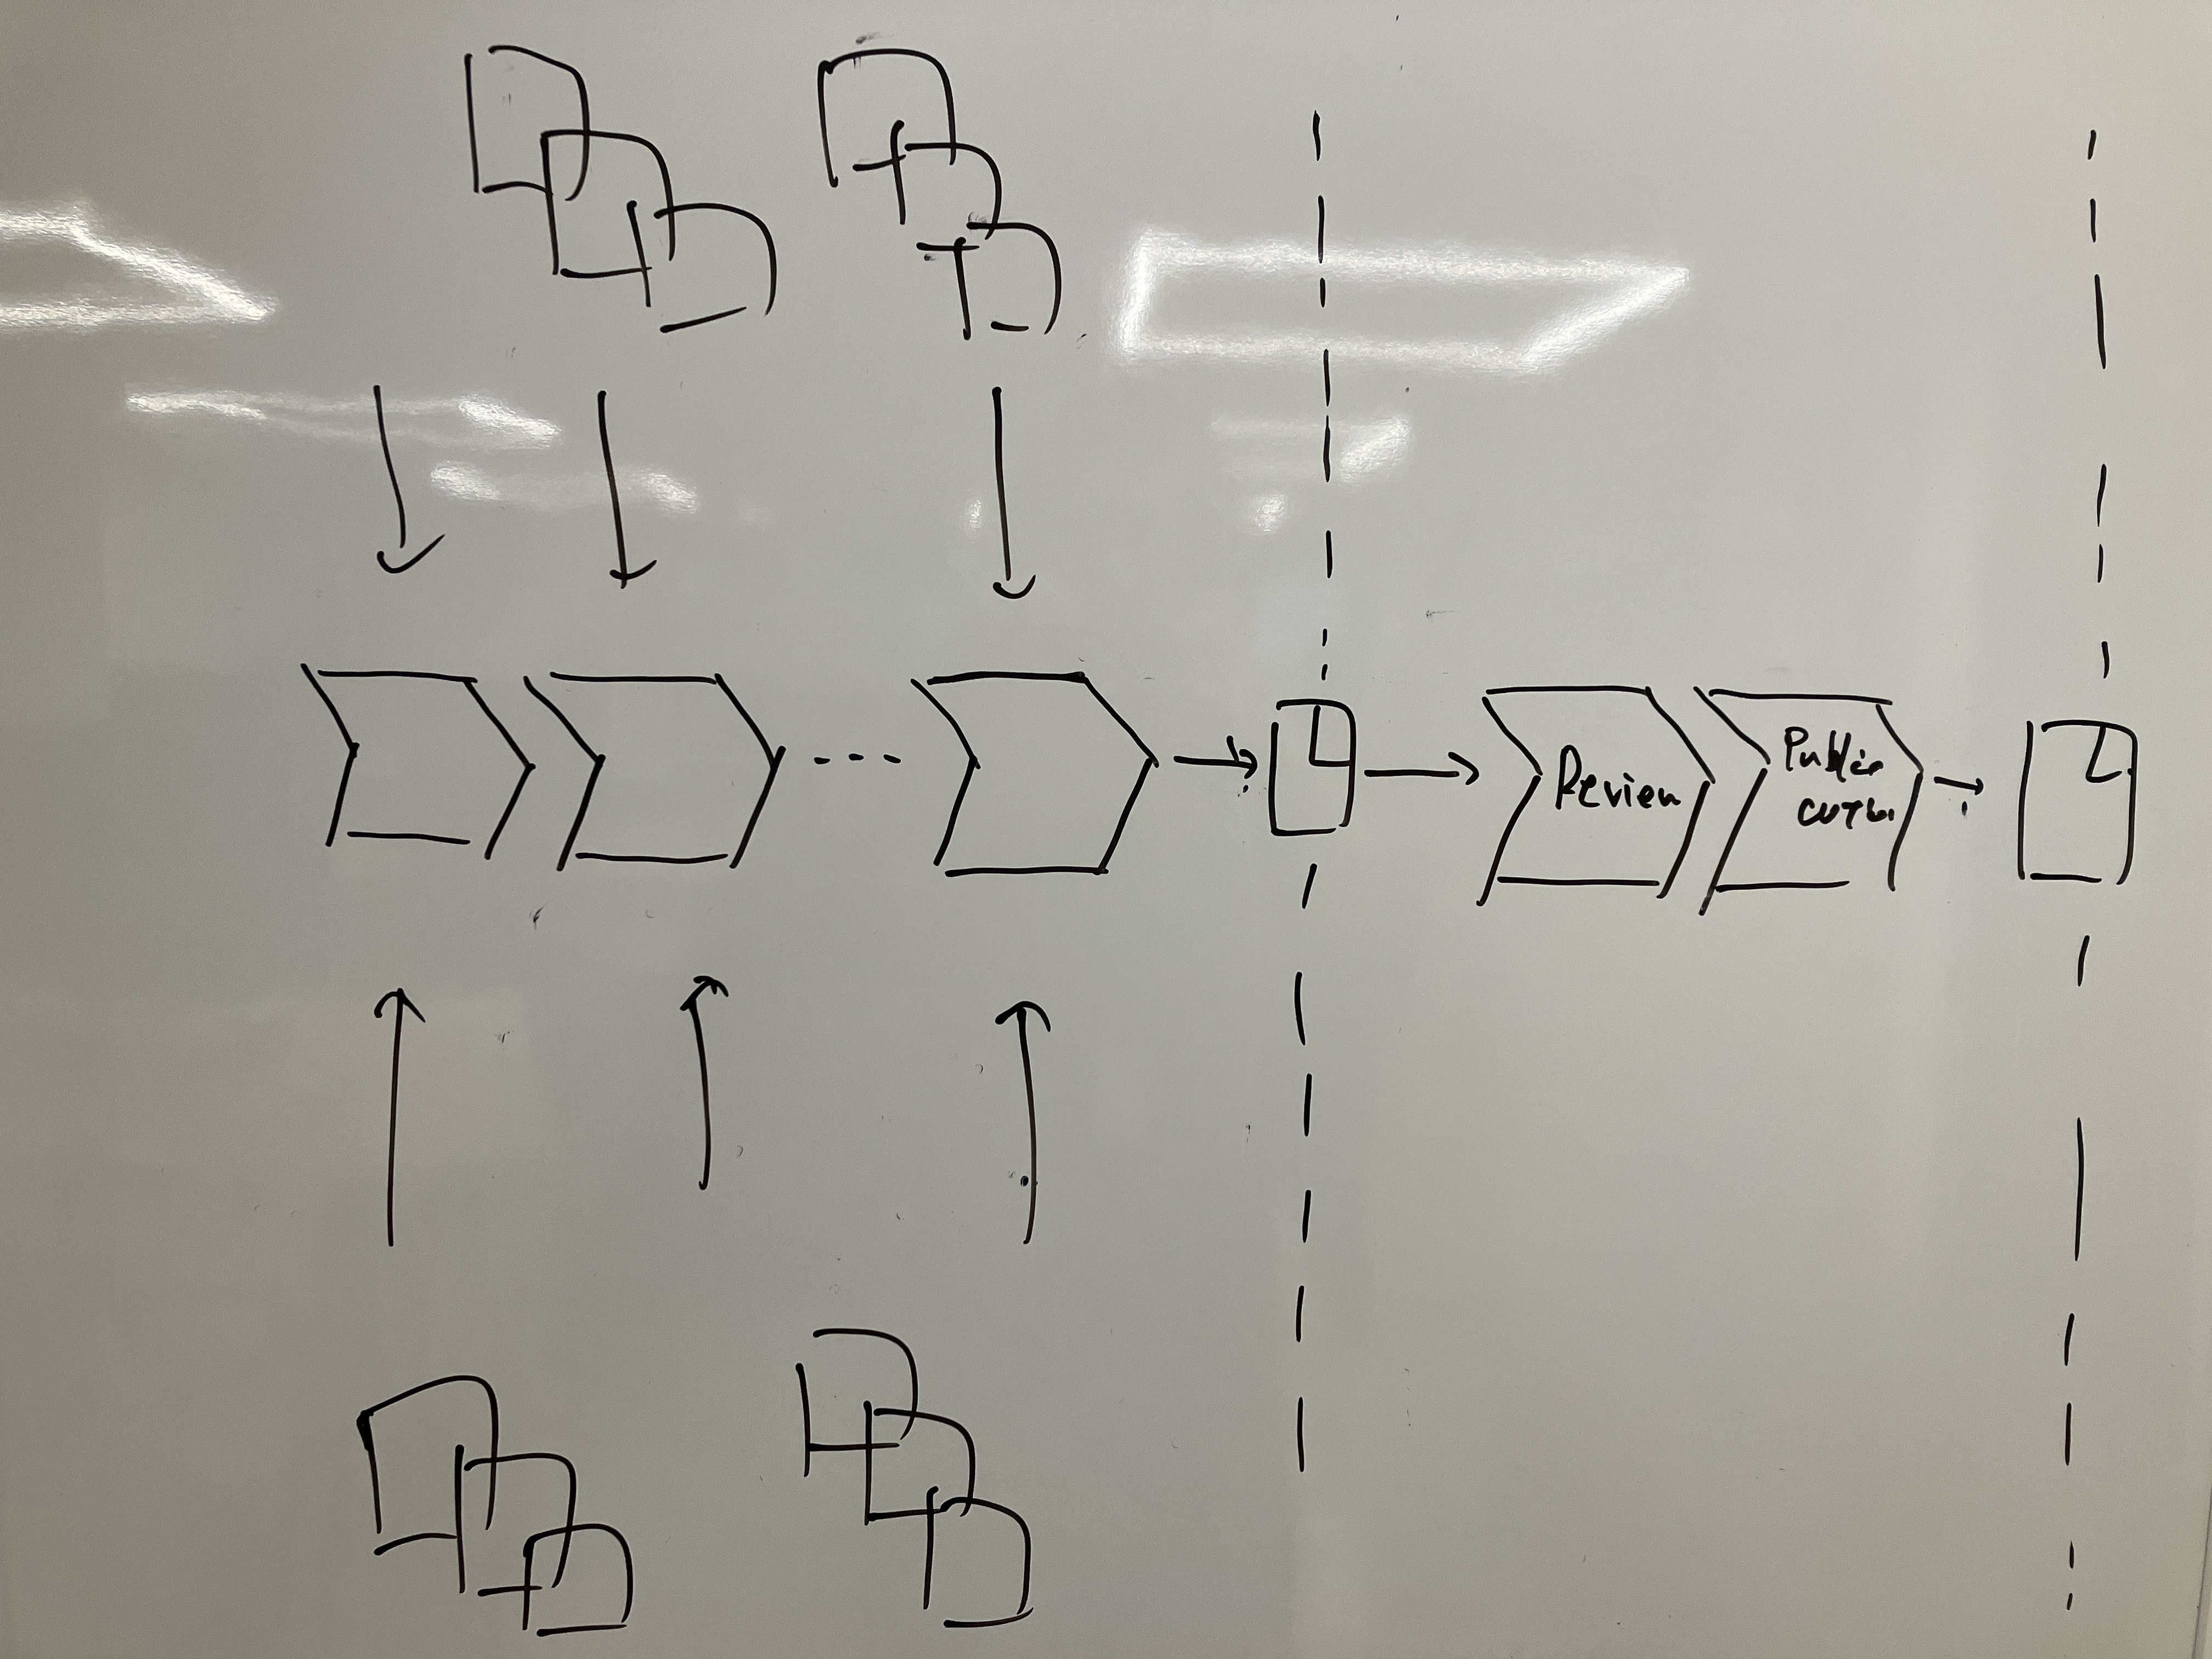
\includegraphics[width=\textwidth]{figs/researchprocess.jpg}
%     \caption{Caption}
%     \label{fig:research_process}
% \end{figure}


% Next, I will discuss a high level description of how human beings have been conducting research. I'll structurize the abstract pattern of the process (which I will call\textit{ research process}) from determining the unknown to it turning into known. 


% \subsubsection{Note}

% note, direction
% Though my structuring may seem to represent scientific methods, I believe this pattern cam apply to other research fields, such as mathematics and humanities as well. When describing the structure, I will make a conscious effort to clearly distinguish between essential elements for knowledge production and those that are not. As previously mentioned, because humans are currently the primary knowledge generators, there are many constraints that come from human society. When considering the possibility of machines conducting research in the future, it will be important to distinguish and organize what is dependent on humans and what is not.

% I believe that the conduct of human research activities can be roughly divided into three stages: knowledge production, knowledge evaluation, and knowledge sharing. 

% Although these may not necessarily be distinctly separable from each other, I adopt this classification because it is useful for advancing discussion. The process of knowledge production consists largely of the steps: problem determination, hypothesis generation, and hypothesis verification. And in this process, the ability to read and write documents and analyze data are required as necessary skills. Below, I will examine each of these in more detail. 


% This structuring is tentative and there may be a better way to structure the research process. However, I have created this structure for practical purposes in order to move the discussion forward. I hope the structure of this article be a starting point for conceiving a better structurization. I believe that structuring and deepening understanding of the elements that are essentially important for knowledge production is extremely crucial when aiming for the automation of research.

% Though I explained that research is belied revision, it would be convenient to see as a function that takes the unknown as input and outputs the known.  % TODO: rearrange

% \subsubsection{Three Sub-Modules in Knowledge Production System}
% In the following sections, I will explain three essential elements that I think are functionally necessary in knowledge production: \textit{question construction}, \textit{hypothesis generation}, and \textit{hypothesis verification}. These are the abstract structure of the research process that has been emphasized so far.


% \footnote{
% While the term ``verification'' is used here, it does not imply a definitive determination of the truth or falsehood of propositions. It is used in the sense of just strengthening beliefs as used in everyday language. Thus, ``confirmation'' may be a more accurate term, but verification is more widely recognized, so I will use that.
% }

% When summarizing these intermediate steps, it goes as follows: First, upon receiving any input, I formulate a question. Taking this question as input, hypotheses are generated. Finally, these hypotheses are input and validated resulting in the creation of knowledge as a research outcome. These processes are considered a proper decomposition of the research process, as they request each other's outputs as inputs and seamlessly connect the entire research process from input to output without any gaps.
% \textcolor{red}{TODO: However, I can identify discovery with justification because both are belief updates. I'll add this point wherever in this paper.} Fig. \ref{fig:knowledge_production_system}.

% \textcolor{red}{TODO: Add fig like this. add this sentence to the explanation of the fig "we approach the unknown to the known by asking questions, providing tentative answers to them, and then verifying the validity of those answers. " }.
% Fig. \ref{fig:research_process}.

\subsection{Question Construction}

The first element is \textit{question construction}. In order to produce new knowledge, one must be aware of what they don't know and strive to generate that unknown knowledge. This process of deciding the unknown to be investigated can be regarded as questioning. And generating the candidates of the answer for that question is hypothesis generation. That is, research may be rephrased as the act of posing questions and answering them. Moreover, as long as there is an attempt to reduce uncertainty, questions are necessary, and we generate multiple questions in the process of research other than the research question. Thus, in the act of research, which confronts the unknown, question construction is inevitable.

In relation to efforts concerning the generation of questions by machines, there are studies aimed at discovering research questions and challenges from academic literature \cite{lahav2022search,liu2023creative,oppenlaender2023mapping,surita2020can}, and others focused on identifying research trends \cite{krenn2022scientific,krenn2022predicting}. However, efforts to let machines autonomously generate questions on their own are not as prevalent. In the field of question answering, there is a task for generating questions \cite{pan2019recent,zhang2021review}, but these studies have different motivations than generating research questions. There has been research on creating artificial curiosity to generate non-textual questions \cite{schmidhuber1991possibility}, but there is yet nothing that can generate research questions like a human. With the advent of large-scale language models in recent years, there have been attempts to generate research questions \cite{liu2023creative,lahat2023evaluating}, but this field is still in the early stage.

While the attempts for automation exist, compared to the those for generation and verification of hypotheses, these efforts are limited. Automating the construction of questions, or setting the goal behind, is recognized as a challenge that needs to be addressed in research automation research \cite{coley2020autonomousII,zenil2023,kitano2021nobel}. In this section, I would like to start by reviewing what questions are and what it means to pose a question in the first place. Them I would extend the discussions to open problems to realize an AI to do research.

% As for attempts to formalize the discovery of problems in the field of machine learning, there is work by Zhang \cite{zhang2021problem}. On the other hand, in this section, we aim to examine the characteristics by qualitatively emphasizing aspects related to the generation of research questions.

\subsubsection{What is Questioning?}
Asking questions seems to be defined as an information seeking behavior \cite{watson_2021,taylor1962process}. The act of seeking information is considered to consist of two steps: recognizing an \textit{information need} and then taking action to acquire that information \cite{wilson1997information,case2016looking}. Not all information-seeking behaviors involve linguistic expressions \cite{watson_2021}, but in research, we always form a query expressed in text between the steps of the information need recognition and the onset of information seeking behavior. Especially, in research, the process of question construction generally seems to refer to the process leading up to this query formulation. Therefore, in this paper, we regard question construction as the process leading up to the query formulation. The subsequent process of seeking information will be treated as part of hypothesis generation and verification.

The process of recognizing an information need appears to involve at least two sub-processes: recognizing the missing knowledge and deciding to fill it (judging that missing information is ``need'').\footnote{
Here, I explained the process of recognizing information need as first determining something as unknown and then deciding if you construct question about the unknown. However, the order doesn't matter. For instance, there may be knowledge that you want to know first, and then you confirm subsequently that it is indeed unknown. What matters is that the process involves these two elements.
} Therefore, to have an AI to construct questions, it would be necessary to consider how to instill these abilities to the AI. In the following sections, I will discuss these steps. However, please note that the question in research is not a personal one, but a question for society. This difference can bring about slight variations in the process of constructing questions. I will touch upon this point again later.

% 情報ニードを認識するという過程は、少なくとも、未知を認識することと、それを埋めことを判断する(欠落した情報がニードであると判断する)という二つの過程を伴うように思われる。したがって、これらの過程について検討する。

% Questioning seems to be an act of trying to fill a gap in the information that the questioner possesses. For example, a philosopher Watson defines a question as an information seeking act \cite{watson_2021} and curiosity, a concept related to questioning, is defined as intrinsically motivated information seeking \cite{kidd2015psychology}. In that sense, the act of trying to produce missing knowledge for humanity is the very act of posing and answering a question. In this paper, we provisionally consider that constructing questions in research is an act of seeking missing knowledge.

% The process of questioning seems to involve two steps: 1. Recognizing missing information, and 2. Attempting to fill that gap. For example, the process of asking why the sky is blue starts as follows: when prompted by, for example the vision of sky to your eyes, you suddenly (with complex perceptual and cognitive processes) realize that you don't know why the sky is blue, and then, if you would like to know the answer, utter the question, ``Why is the sky blue?'' Therefore, to have an AI to construct questions, it would be necessary to consider how to instill these abilities to the AI. In the following sections, I will discuss these steps.\footnote{
% Here, I explained the process of questioning as first determining something as unknown and then deciding if you construct question about the unknown. However, the order doesn't matter. For instance, there may be knowledge that you want to know first, and then you confirm subsequently that it is indeed unknown.
% }

\subsubsection{Recognizing Unknown}
To recognize that certain knowledge is unknown to you, it seems necessary to first attempt to refer to that knowledge. It appears that when we refer to our own knowledge base and do not find the knowledge, we judge it to be unknown. For an individual, the knowledge base is the memory within the brain. On the other hand, the unknown researchers wish to clarify is unknown to a certain society. That is, a research-capable AI does not need to judge whether it is unknown to itself, but rather it can directly determine whether it is unknown to certain society. Therefore, the knowledge base can be not only its own memory but also the knowledge base of the society, e.g. a collection of research papers.\footnote{
As previously mentioned, being unknown means that a proposition either does not exist or, even if it does, it is not accompanied by a justified belief. Therefore, it seems that in order to precisely determine unknowingness from academic papers, it seems to be necessary to judge whether each paper has been justified, that is, whether verification has been appropriately conducted. 
}

% It seems that in order to recognize that certain knowledge is unknown to you, you need to attempts to reference that knowledge and finds it unavailable to you. When prompted with a request for a specific type of knowledge and upon referencing your own knowledge base, if you judge that you do not possess that knowledge in your knowledge base, you recognize it as unknown to you. For example, ``why question'' is driven by the request of the knowledge of ``reason'' or the ``cause''.\footnote{
% Such demands for knowledge would likely be triggered by various factors (for example, attention may be drawn to the causal relationship between the sky and its blueness because one tried to explain why the sky is blue but couldn't). Identifying the mechanism of what and how questions are prompted remains an open problem with no answer yet.
% }

% For an individual, the knowledge base is the memory within the brain. If certain knowledge is not in the memory, or cannot be constructed from other knowledge that is in memory, we would recognize that we don't know that knowledge. 

% In research, what interests us is not whether something is unknown to an individual, but whether it is unknown to humanity. Thus, the knowledge base consists of the collective media that records human knowledge, such as the research papers. If we examine as many academic papers as possible and find no prior research that has presented a properly validated hypothesis for the same question, we recognize that knowledge as unknown.\footnote{
% As previously mentioned, being unknown means that a proposition either does not exist or, even if it does, it is not accompanied by a justified belief. Therefore, it seems that in order to precisely determine unknowingness, it seems to be necessary to judge whether each paper has been justified, that is, whether verification has been appropriately conducted. 
% } Even in a world where machines conduct research, this method of determining unknowns will likely persist.

If machines would determine the novelty in a research survey like humans do, then it might not be a problem. However, there is a question as to whether we should consider something as unknown to us if a machine determines it to be unknown based solely on its own memory. Such judgment may sound reliable if the AI was pre-trained with all scholarly papers. However, as mentioned before, just because AI deems something unknown, it doesn't guarantee that it's unknown to humans. This issue is an open problem.

% philosophy of literature survey \cite{schryen2015theory}

\subsubsection{Deciding What Knowledge to Seek}
We do not always formulate questions for everything we don't know since not all unknowns are equally ``important'' or ``interesting'. Instead, we construct questions for things we wish to know the answers to. This means that we assess some ``value'' of questions using some criteria to determine if it is worth pursuing. For individual, this can be an unconscious internal process, but for research, this doesn't need to be so as long as it is some value judgment process.

Knowledge in itself is value-neutral. The ``value'', ``significance'', or ``goodness'' of knowledge is determined by those who using it. The crucial point here is that the criteria for determining ``value'' are arbitrary. Therefore, if we want AI to pose questions that are meaningful to humanity, we should recognize what is ``good'' or ``significant'' questions and instill and make AI adhere to such values. 

However, we should also be mindful that there might be questions that we would judge as ``unimportant'' but are actually ``important'' under some criteria. For instance, there is a myriad of knowledge born from fundamental research that, at first glance, might seem ``useless'' but actually leads to later innovations. Due to human cognitive limitations, there might also be instances where we cannot fully assess the utility of that knowledge. Additionally, in human society, sometimes social factors unrelated to the original purpose of the knowledge production influence value judgments. That is, our value judgments are not necessarily always optimal.

Since AI is not bound by such constraints, there's a possibility it can make better value judgments. Therefore, while it might be essential to provide some minimal guidance to ensure AI generates questions meaningful to humans, it would be good to aim for the development of AI that can autonomously construct good value criteria by themselves. How to create such an AI seems to be one of the important open problem in building an AI capable of research.\footnote{
Kitano referred to the science in which humans adopt their own value judgment criteria to determine questions and hypotheses as \textit{value-driven science} \cite{kitano2021nobel}. He argued that advancing \textit{exploration-driven science}, which focuses on more comprehensive and thorough exploration rather than criteria based on specific human values, is important for societal development. Although a completely value-neutral system would be impossible, I agree with the idea that employing new and diverse criteria would matter for future research. By adopting more diverse and extensive criteria, we could expand the exploration space of knowledge.
} 

\subsubsection{Origin of Information Need}
I explained that the question begins with the recognition of an information need. So, what causes the recognition of an information need (or the sub-processes of the recognition of unknowns and the judgment of value) in the first place?

Various factors can be considered as triggers. Some people may generate research questions as they logically think about how to achieve a goal. Others might come up with a question upon noticing some anomaly while observing experimental data or realizing that there might be something wrong with the underlying assumptions based on a discrepancy between results deduced from some assumptions and actual observational data. Furthermore, in reality, humans do not evaluate based on a single criterion of value judgment. It seems that they combine these criteria in a complex manner, weighting them according to the situation, before arriving at a final value judgment.
If one wants to create an AI that can autonomously construct research questions like humans, it seems necessary to develop an AI with a general methodology that can construct questions in any of these situations.

How these various factors are connected to information need in humans, and how we can create an AI capable of this, remains one of the most important questions and is still an open problem. Researchers studying curiosity have been tackling this difficult problem. Curiosity, while it is difficult to precisely define, is viewed as \textit{a drive state for information} \cite{kidd2015psychology}. In this sense, curiosity can be considered as something that gives rise to an information need. Indeed, especially in the process of information-seeking, it is characterized as one of the precursors of information need \cite{case2016looking}. Efforts to instill curiosity \cite{schmidhuber1991possibility} or knowledge-based intrinsic motivation \cite{oudeyer2007intrinsic} in artificial intelligence have been researched in the field of reinforcement learning. There, curiosity is formulated as novelty, information gain, or prediction error, and is perceived as something that encourages exploration \cite{aubret2019survey}.

These efforts have provided guidelines on how to implement mechanisms that drive intelligence towards questions. However, we are still halfway to realizing a system that autonomously construct research questions under complex value judgments in all situations, as humans do. Especially, while a question becomes the minimum input in hypothesis generation, and a hypothesis in hypothesis validation, in question generation, it's unclear what the minimum input should be. Need to design a complex internal driving force adaptive in various situations seems to be a major difficulty for creating an autonomous research questioner. Identifying what is necessary to realize such AI is an important open problem.
% これらの取り組みは、知能を問いに突き動かす機序をどのように実装するかについての指針を与えてくれました。しかし、依然として人間のようにあらゆる状況で複雑な価値判断のもと研究対象となるような問いを自律的に生成するシステムの実現にはまだ道半ばです。特に、仮説生成であれば問いが、仮説検証であれば仮説が最低限の入力となるのに対して、問いの生成ではそのような最低限の入力が何か分からず、自律的に問いを生成するには内的報酬のようなうまい機序を作らなければいけない点が大きな困難であるように思われます。このような AI を実現するためには何が必要なのかを明らかにしていくことは重要なオープンプロブレムの一つです。

% One of the challenges in trying to create an autonomous research question constructor is determining how much input humans should provide to the AI and to what extent humans should design the mechanism for constructing questions. For example, the minimum input for an AI constructing questions for a goal is the goal itself. However, a goal might not be the minimum necessary input for other types of question generation methods. Also, as is often discussed in the context of research automation, if one aims to make the AI autonomously generate even goal itself, we would likely necessitate assuming even more primitive inputs for it, e.g. higher-level goal.

% For creating an autonomous artificial researcher, it seems important that these are driven by intrinsic motivations. However, it doesn't necessarily have to be intrinsic motivation in the commonly understood sense. In the context of research, intrinsic motivation often seems to be associated with feelings like ``interest.'' But, as we'll discuss later, the motivations for posing questions can be diverse. For instance, questions could be framed for the purpose of optimizing some externally set metric. Therefore, if we narrowly define intrinsic motivation in this way, it might be argued that an AI capable of research doesn't necessarily need to have curiosity.

% Of course, if we take a broader view of intrinsic motivation, considering it akin to the evaluation function an agent possesses, then an autonomously inquiring AI is essentially the same as a curious AI.


% Research do not always have to be intrinsically motivated.

% curiosity is intrinsically motivated information seeking \cite{kidd2015psychology}

% theory that people decide what information to seek by considering the positive and negative effect of it to their action, affection, and cognition \cite{sharot2020people}

% curiosity -> exploration \cite{oudeyer2018computational}

% book of intrinsic motivation \cite{baldassarre2013intrinsically}



% This is because the essential requirement for research is that the answer to the question is unknown, and in principle, I do not require additional properties question to have. For example, you can ask about anything if it is unknown, or you can choose to ignore it if it's not intellectually intriguing. Alternatively, you can opt for something that seems to lead towards a specific goal you are pursuing. This has a critical implication for aiming to automate research. If the value standards are always given by humans, then there is no issue. However, when considering the possibility of automating even that aspect, it becomes necessary to discuss how I can make it adhere to the desired criteria. While it is natural to want them to ask ``good'' or ``important'' questions, it also becomes challenging when it comes to thinking about this issue. Let us discuss this further in below.

% I claimed that the value judgement is arbitrary. This is because the essential requirement for research is that the answer to the question is unknown, and in principle, any question is valid. In light of the definition of knowledge production, value judgement is not necessarily required for knowledge production to be as it is. From the perspective of knowledge production, as long as the unknown is truly unknown and it be rigorously approached towards becoming known, there should be no problem. The unknown can be anything arbitrary, and knowledge production itself does not demand a specific nature for it. 

% % \subsection{Relativity of Value}
% Knowledge in itself is value-neutral. The value, significance, or goodness of knowledge is determined by those who using it. 


% The value of knowledge is inherently dependent on context, so the significance or goodness of a certain knowledge is not determined a priori from the moment it is generated. Goodness becomes an issue only when that knowledge is used by some member of the society in some form. In other words, the demand for importance and goodness is a constraint imposed by society not by knowledge production. For example, certain knowledge may be considered ``important'' in the sense that it addresses the interests of all the researchers working on similar topics, providing solutions to their concerns. Alternatively, that knowledge might be deemed ``important'' to someone simply because they find it intellectually interesting. On the other hand, if it takes a considerable amount of time for this knowledge to translate into practical applications, it may not be considered ``important'' to someone who wants to start a business immediately. Hence, this is the choice of us (or them) on what objective I would like to maximize by knowledge production.\footnote{
% The fact that the value is arbitrary and not necessary condition for knowledge production doesn't mean I do not have to discuss about the value. In the first place, it is inherently impossible for all actions to be value-neutral. So it is inevitable for us to conduct some value judgement. Moreover, the realm of possible unknowns is too vast, so without any constraints, only nonsensical questions would arise. Most of us are interested in ``good'' or ``important'' questions. So, what I should consider is how to identify them and how to instill them to machines.
% }

% This provides important implications when attempting to create an artificial intelligence that autonomously conducts research, at least in two aspects. Firstly, if I am interested in making machine autonomously construct ``good'' question for humans, I should consider what is ``goodness'' for humans and how to instill them to machines. However, it seems that I have not yet fully established a unified common understanding of what constitutes a "good" question. ``What makes a question good for humans'' and ``how to formulate them effectively'' are crucial aspects that require further in-depth discussions. Therefore, I will revisit and explore these important points separately later on.

% It seems that I still lack an understanding of what kind of research questions are important, but in the field called \textit{science of science} \cite{wang2021}, which studies the research itself, scientific studies on research impact are also advancing. The insights gained here may provide important knowledge in building new algorithms and optimization metrics.

% The second implication when attempting to create an artificial researcher is that if I do not intentionally impose any constraints, there is a possibility that the intelligence produced may not align with the knowledge I desire. This is an important point and thus will be discussed in a separate chapter.

% Secondly, it suggests the possibility of adopting values that are different from the ones I currently employ can result in better knowledge production. I have explained that I make judgments about certain questions being good or important based on some criteria or standards. However, there may be questions that are not considered ``important'' according to current criteria but actually be extremely significant. As mentioned earlier, the value of knowledge is determined by its usage and context, and it can vary over time and in different environments. Therefore, it is highly challenging to determine the importance of knowledge during the stage of knowledge production. Even in the same environment, it is difficult to assess the significance of knowledge. This is because knowledge results from complex accumulations, leading to new insights, and there is a intricate chain of connections before a particular knowledge becomes recognized as important within a society. In addition, I am bound by various cognitive limitations inherent to being human. Therefore, I can only assess the importance of knowledge within the confines of these limitations. 

% Given these circumstances, it is highly possible that the current adopted criteria for value judgments are missing out on the production of potentially important knowledge. The development of knowledge production systems that embrace new value judgment criteria can be expected to increase the potential for generating such knowledge by expanding the scope of exploration. If an artificially intelligent system capable of autonomous research is developed, it can be expected that research based on these new criteria will become more feasible. This could potentially enable the resolution of many previously unsolved problems that were not attainable before.

% As a conclusion, let us emphasize again that I first need to be aware that these ``good'' aspects do not occur naturally. To create an intelligence that constructs ``good'' questions, I first need to understand what I consider a ``good'' question. Also, it's important to turn my attention to things that are not currently considered ``good,'' but should be deemed as ``good'' in essence. Only then can I discuss how to align that value with the agent. Therefore, I think I should start by listing the criteria for determining the ``goodness'' of a question. 

% For this, discussions in the philosophy of science and meta-sciences like the Science of Science may be referenced. Alternatively, large-scale surveys of researchers engaged in actual research could also be important. Once the value is clarified, I might be able to think about creating an intelligence equipped with these values using the value alignment techniques that are currently being developed.

% Science based on the importance of questions discussed above is a \textit{value-driven science} \cite{kitano2021nobel}. However, as previously mentioned, these may be due to cognitive constraints imposed by human society, including the inability to handle knowledge that is deemed ``unimportant.'' Therefore, when automating question generation, it may be possible to explore a wide range of questions, including those that were previously considered ``unimportant.'' In doing so, it is possible that knowledge that was not considered ``important'' according to previous criteria could actually be extremely significant. This is referred to as \textit{exploration-driven science} \cite{kitano2021nobel}, and it could become a new form of research liberated from constraints imposed by humans. 

% Indeed, it is impossible to create a completely value-neutral system. All agent systems must have some form of bias. However, what I would like to emphasize is the potential to incorporate biases different from the criteria previously used by humans, and how this can enable us to consider more diverse approaches to research. This highlights the importance of creating agents capable of autonomously conducting research.

\subsubsection{What Are the Criteria for the Value of a Research Question?}

% \subsubsection{Diverse Good Research Questions}
So far, I have discussed somewhat abstract topics related to questions in general. Now, I would like to discuss the characteristics related to research questions specifically, and how humans judge the value of these questions. 

The ``quality'' of a research question can be judged based on various criteria. I will introduce some examples from among them to make it clearer how humans have determined the value of a research question. Please note that the following examples are just a few of the many criteria humans use to judge the value of a question and are far from comprehensive. I hope this will aid in further deepening the discussion on how humans determine the value of a question.

The idea that questions which would bring about new perspective or understanding, or \textit{conceptual advance}, especially which would overturn our common sense or underlying assumptions are important is widely accepted within the research community. As an example, Alvesson and Sandberg point out the importance of these kind of questions and discuss the strategies to construct them \cite{alvesson2013constructing}. 
This criterion is based on the premise that a good question is one that produces knowledge which has a significant impact on our current body of knowledge.

No matter how significant a question is, if it's nearly impossible to address with current technology, producing meaningful research outcomes from that question may be infeasible. Therefore, some argue that the feasibility of answering a question should be considered when evaluating its quality, with questions that are not overly implausible being deemed good ones \cite{hulley2007designing,alon2009choose,huntington2021effect}. To determine feasibility, it seems that complex decision-making is necessary, as it requires consideration of various factors such as the resources and funding currently accessible, the capabilities of the researchers, deadlines, and even the limitations of the technology currently available to humanity. In reality, an AI capable of conducting research would likely need to be able to make such complex decisions.

The notion that research questions should be based on an individual's intellectual curiosity also seems to be widely accepted. Curiosity is the driver of exploration \cite{oudeyer2018computational}, so curiosity-driven research might have promoted exploration in the research theme space. Research can be seen as an exploration of the space of truths in this world, hence it sounds reasonable that value standards that promote exploration are important.
To discover things that are so unknown they are not even known to be unknown, exploration is essential as an entire endeavor of science."
Conversely, the criteria should not necessarily be curiosity as long as it promotes the exploration in the space of knowledge. The exploration driven by curiosity is merely a byproduct, and there may exist better heuristics for exploration. If AI acquires such value standards, it might be able to unravel truths more efficiently than humans have done.

% To construct such questions, we generate hypotheses by repeatedly engaging in question and hypothesis generation.\footnote{
% For instance, let's say we have a goal of ``creating AGI''. Initially, we pose the question, ``How can we create AGI?''. In response to that, we consider elements necessary to create AGI as our hypotheses. For example, we might think, ``Realizing an AI capable of logical reasoning, an AI with embodiment, etc., might be necessary.'' Then, we ask, ``How can we create an AI capable of logical reasoning?'' and consider hypotheses for that question, and this process is repeated.
% }

Contrary to research driven by bottom-up curiosity, the notion that questions contributing to the achievement of specific goals set in a top-down manner is valuable is equally common. For instance, for those aiming to realize AGI, questions about how to create elements deemed necessary for AGI would be significant for them, even if it is not interesting or incremental. Especially in corporate research or government-led research, there are likely many studies aimed at achieving goals set in a top-down manner. It is assumed that many people expect AI capable of conducting research autonomously to contribute to goals set by humans. Therefore, the ability of AI to make this kind of value judgment is an important requirement.

Lastly, there is also a perspective that emphasizes the value for individual. Alon expresses the view that a good research problem is one that is interesting to the individual and has an appropriate level of difficulty for them \cite{alon2009choose}.

In reality, instead of adopting just one of these criteria, we determine the value of the research question by comprehensively considering multiple criteria. For example, Hulley et al. suggest that questions that is feasible, interesting, novel, ethical, and relevant (FINER) should be considered good ones \cite{hulley2007designing}. Huntington-Klein presents the view that good research question is answerable and the answer to the question will improve our understanding of this world \cite{huntington2021effect}.

As already mentioned, these are just a part of the value judgments that humans make in determining questions. I hope that future discussions will delve deeper into what kind of value judgments humans make, what function they serve in scientific discovery, and how we can realize these functions in AI.

% Gap spotting vs problem solving \cite{alvesson2013constructing}

% Up until now, I have been explaining that values like goodness are relative and subjective. However, it is natural for artificial researchers to autonomously construct ``good'' or ``important'' questions. While I admit that adopting diverse value criteria and not being bound by traditional standards matters as Kitano said, even in that case I still have to determine a criteria that lead to ``good'' questions in some sense. Therefore, I would like to discuss what constitutes a ``good'' question for us and how I can construct such questions, drawing upon the discussion of how I have characterized ``good'' questions thus far.

% \subsubsection{Goal Oriented Question}
% One of the most general, significant, and widely accepted criteria for what I consider as ``goodness'' is that a question is deemed ``good'' if its answer contributes to achieving a desired, yet unrealized, goal. This is because researchers often seek to address long-term problems and engage in knowledge production for that purpose. For instance, physicist who pursue a unified theory would think that a question that furthers the realization of a unified theory is a good question. This can be referred to as a \textit{goal oriented research question}.

% In this approach, we first set the ultimate objective. Then, we identify the most critical bottlenecks, or sub-goals, that are essential to achieving that objective. We once again consider sub-goals for these identified bottlenecks. This process is repeated, converging on more specific and feasible sub-goals that are of high importance. Finally, I frame the question to address these sub-goals as the research question. 

% For identifying the knowledge required to achieve the ultimate goal, we typically start by listing the necessary elements to accomplish it. For example, to achieve general artificial intelligence, we may think that it requires the ability to handle language, understand the real world, be proficient in systematic reasoning, and align with human values, etc. 

% Then, we break down them again into the necessary things to achieve the them. For instance, to understand the real world, for instance, we may need the capability for interacting with the physical world, processing visual information, and so on. These requirements can be further broken down into multiple necessary elements. By repeating this process, we can narrow down the specific tasks that can be directly addressed. Then, the required knowledge to accomplish those tasks is demanded, and that's where it directly connects to the research question. The process is conceptualized in Fig. \ref{fig:unknown_tree}.


% \begin{figure}[htb]
%     \centering
%     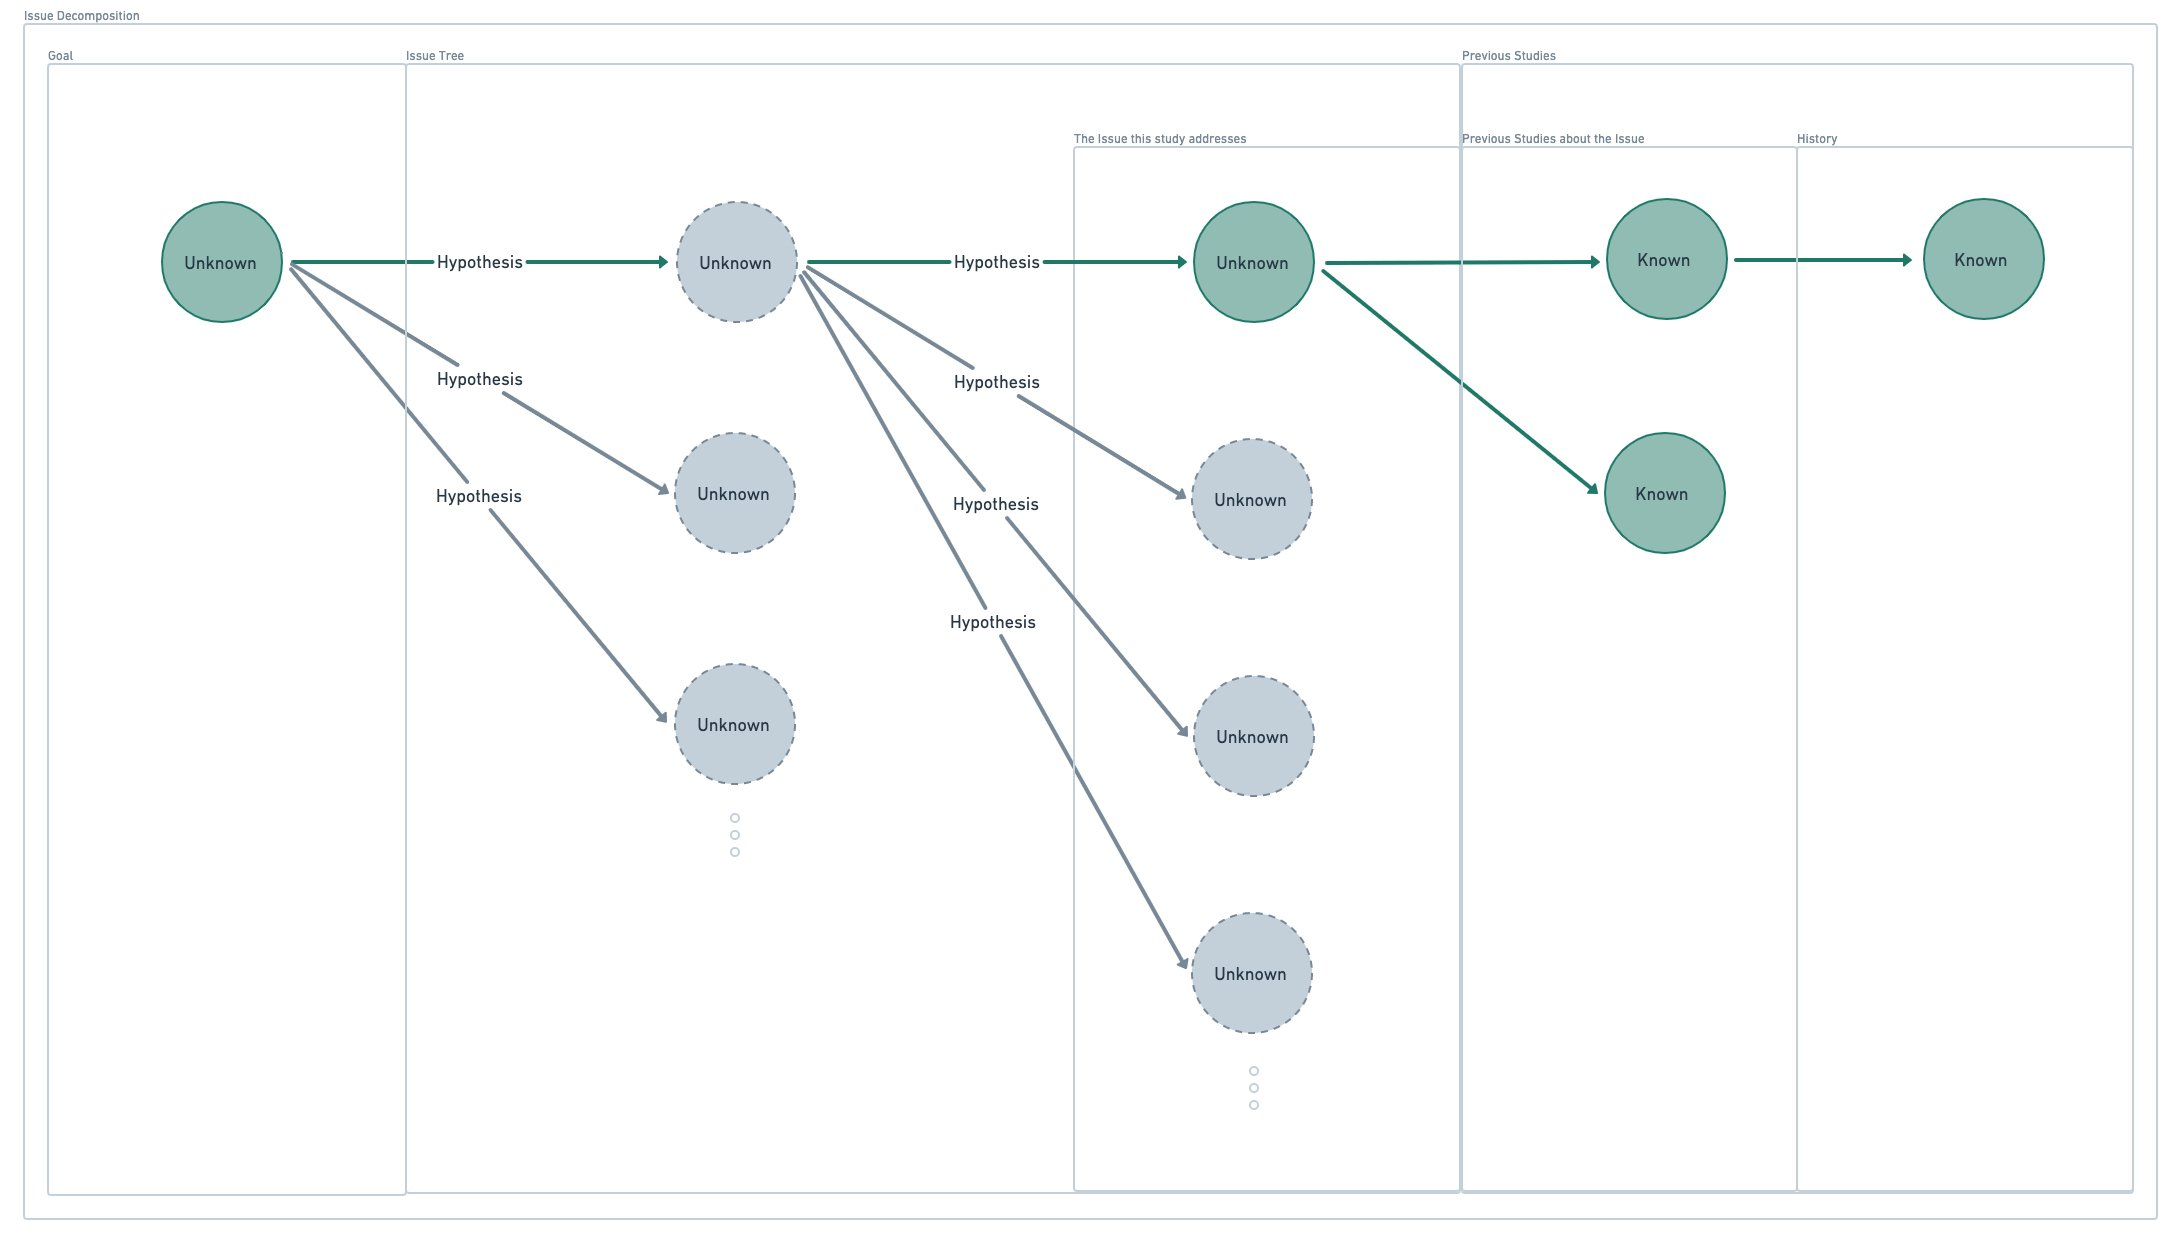
\includegraphics[width=\textwidth]{figs/unknown_tree.jpeg}
%     \caption{Caption}
%     \label{fig:unknown_tree}
% \end{figure}

% Several things are happening here. Firstly, listing the elements necessary for achieving the goal means generating sub-goals from the main goal. However, it's always a challenging problem to evaluate how a particular sub-goal contributes to the achievement of a given goal. Especially in the case of research, the target might be an too general and ambitious vision that nobody has achieved before, so I need to think about what needs to be done to break it down into appropriate sub-problems. In other words, it is necessary to construct a tree with nodes representing sub-goals. Namely, this is the tree of repetition of constructing a question and generating multiple hypotheses without verification. I will delve into the discussion of hypothesis generation in the next chapter, so I won't go into the details here.

% Secondly, it is necessary to identify the most important and feasible sub-goal from the selected candidate sub-goals. This is because only one question can be addressed in the end. However, assessing and comparing sub-goals is a challenging task since I have no experience to realize the ultimate goal and so have no data what sub-goal actually is the most important.

% Thirdly, the question to ultimately arrive at must be verifiable. If the question is not specific, meaningful verification cannot be performed. Overly broad or ambiguous questions can result in countless or trivial answers, or they may be too unclear to provide practical answers. Increasing the specificity of the question corresponds to deepening the depth of the sub-goal tree, so it may be important to construct a sufficiently deep tree and find an efficient way to navigate it. The verifiability is constrained by the knowledge, resources, such as funding and technology, that I currently have. Therefore, when conducting verification in reality, it is necessary to consider such feasibility. Whether to tackle a question with high feasibility or to further divide it into more sub-tasks for its realization is a matter of judgment. In any case, it is necessary to appropriately evaluate such feasibility. The scope of feasibility is vast, so it is a challenging problem to determine how to consider it in creating intelligent systems.

% In this discussion, I considered the method of outputting questions from the goal through the construction and exploration of a tree structure. However, as mentioned by the predecessors, if an end-to-end approach ultimately becomes a powerful method, it may be more desirable to consider a direction in which questions are directly output from the goal. In particular, even when performing multi-step reasoning, it seems more natural to improve reasoning abilities using the recently developed approaches to multi-step logical reasoning, rather than explicitly considering tree structures. 

% To pursue this direction in research automation, specifically, it may be worth considering the construction of higher-quality datasets for goals and research questions. For example, it may be possible to construct a dataset by extracting only the ultimate goal and the research questions actually solved from the introductions of papers. However, an important point to note here is that the research questions created by humans so far are not necessarily optimal for achieving research goals. Firstly, machines may be capable of maximizing the objective better than humans due to cognitive constraints. Secondly, not all human research has been conducted by working backward from a clear goal. Some studies were conducted simply because they seemed interesting while reading papers. In this regard, simply learning from human data may constrain the potential capabilities that machines can possess. Therefore, it becomes important to consider how to formulate the maximization of the probability of achieving research goals as a problem, rather than naive imitation learning of human data.

% As evident from the formulation, to construct research questions for contributing to achieve a specific goal, we need to solve long range reasoning problems. This problem is widely studied in machine learning research community to improve the reasoning capabilities of machine learning models and on generate intermediate goals in reinforcement learning. If these research fields produce significant results, they can be directly applied. In this sense, it might be beneficial to seek cooperation from those who are actively conducting research in these areas. One of the unique aspects of long-distance reasoning problems in research automation is that the goal is something that has never been achieved before. This means that you cannot naively learn from data and need to generalize out of distribution. Therefore, it's essential to acquire skills not just to recognize patterns but to properly trace the path of reasoning. Moreover, because the goal has not been realized, sub-goals and the paths that connect them are ultimately based on the accumulation of hypothesis generation. In this sense, it can be said that this is a highly uncertain inference. This implies that the choice of which node to select is far from self-evident compared to other logical reasoning problems. Furthermore, there is the issue of the complexity of the distance between the goal and the question, which is far more intricate than, for example, games or planning everyday trips. For instance, to truly achieve the goal, it may be necessary to build large-scale apparatus like particle accelerators from scratch. This also means that the temporal distance between the goal and the current location is very long. Therefore, it becomes a problem that feedback on how much solving the question contributed to the goal is significantly delayed. While we've only listed a few examples here, there may be other unique challenges and issues that become more serious in research. It will be necessary to work on refining these technical challenges into specific research tasks through discussions with researchers in reasoning and planning.

% \subsubsection{Important but Unnoticed Questions}

% One example of a ``good'' question seems to be one that, in its construction itself, brings benefits to many researchers. By considering why hypotheses regarding the question are unknown, it becomes somewhat clearer what kind of question this is.

% The reasons why the answer to a question remains unknown are diverse. In some cases, the question is simply new, and no one has had the time to come up with an answer yet. For instance, a question about the internet posed on the day it was invented may still remain unanswered because it has only been a day since its birth, and no one may have delved into it yet. In other cases, the question might simply not interest anyone, leading to an absence of answers despite the availability of time. This is an example of a question that remains unanswered because nobody is willing to tackle it, even though time exists.

% Furthermore, there are questions that are difficult, and no one has been able to solve them. For instance, the question of how to achieve human immortality has been contemplated by many, but due to its complexity, no answer has been found yet. Lastly, there are questions that are important for a particular purpose but remain unnoticed by everyone. As previously mentioned, realizing challenging objectives that are yet to be achieved poses difficult problems. In such cases, it is often unclear what is not known or what is at the heart of the problem. In such situations, clarifying the question itself holds great significance.

% Thus, constructing questions of this kind seems to be important as it can help shed light on the unknown. With this in mind, it appears worthwhile to discuss this topic in detail.\footnote{
% Please note that the concept of a question being unnoticed and the answer to the question being unknown are different. The necessary condition for research is that the answer to the question is unknown. 

% If the existence of a question is not known to anyone, then naturally, its answer would also be unknown since no one would have answered it. So, if the existence of a question is unknown, then the answer to the question is also unknown.
% }

% \textcolor{red}{TODO: Add discussion}

% \subsubsection{Diverse Good Questions}
% There have been various discussions on the elements that good research possesses. For example, \cite{hulley2007designing} proposed that good research question should satisfies FINER criteria (feasible, interesting, novel, ethical, and relevant) and \cite{alon2009choose} claims that a good problem is one that is most feasible and interesting to oneself.

% \textcolor{red}{TODO: Add more discussion on ``good'' questions, examples, discussion, what is good, what is important, specific question is good, etc.}
 

% \subsubsection{Where Does a Question Come from?}
% Research questions can arise in various situations. Some people may generate research questions as they logically think about how to achieve a goal. Others might come up with a question upon noticing some anomaly while observing experimental data. Furthermore, as with Kepler, one might realize that there might be something wrong with the underlying assumptions based on a discrepancy between results deduced from some assumptions and actual observational data. If one wants to create an AI that can autonomously construct research questions like humans, it seems necessary to develop an AI with a general methodology that can construct questions in any of these situations.

% One of the challenges in trying to create such a general and autonomous research question constructor is determining how much input humans should provide to the AI and to what extent humans should design the mechanism for constructing questions. For example, the minimum input for an AI constructing questions for a goal is the goal itself. However, a goal might not be the minimum necessary input for other types of question generation methods. Also, as is often discussed in the context of research automation, if one aims to make the AI autonomously generate even goal itself, we would likely necessitate assuming even more primitive inputs for it, e.g. higher-level goal.

% For creating an autonomous system, the question construction module faces challenges due to being the initial building block of the system. This challenge is determining ``what should be the input to the question construction module.''

% Questions do not arise from nowhere. There is always something before reaching a question. In the example I mentioned earlier, for instance, the question may arise as a result of a literature review. Then, why did you conduct that literature review in the first place? It could be because there is a research theme you want to know about in the research field. And then why are you interested in that research theme? It could be because the topic of the first paper you encountered during graduate school was fascinating, or it could be because you have been interested in it since childhood. And there may be causes behind those as well.

% In this way, identifying where a question begins is a hard problem. If you think seriously about it, it will lead to an infinite regress. This is a significant problem when I want to realize an autonomous artificial researcher. As infinite regress can occur, the decision of where to terminate lies solely with the designer, and it is not automatically resolved by creating the system. Can I say that question construction is autonomous if the literature to read were given? Can I say that question construction is autonomous if research theme were given? I believe it is necessary to accumulate such discussions and determine how far to consider something as given, in order to define what qualifies as autonomous.

% In this paper, I assume that a trigger that requests a specific type of knowledge is given. And from there, it makes decisions about determining the unknown and constructing questions. The reason is that discovering questions with unknown answers is a necessary condition for research, and I believe this is the minimal requirement for it. However, one could also try to automate even the aspect of requesting a specific type of knowledge. The reasons for expecting the existence of certain knowledge can vary and are arbitrary. For example, I might have an objective and first consider what I need to do to achieve it. I then anticipate the necessary knowledge to accomplish those tasks. This corresponds to the demanding for a specific knowledge.

% As an another example, let's consider the case of a child asking, ``Why is the sky blue?'' In this case, the child may already have prior knowledge of the concept of ``sky'' and ``blue.'' Additionally, they may possess a naive concept of causality, believing that ``A is B, so there must be a reason for it.'' Thus, they may have expected to have the knowledge that ``the sky is blue because of B.'' However, when they reference their internal knowledge, they find that it does not contain the corresponding knowledge. Therefore, they may have asked the question ``Why is the sky blue?'' to evoke the knowledge they were lacking. In this case, the required knowledge is ``the sky is blue because of B.'' and this is induced just because the result of children combining known concepts.

% The question of ``why do I seek information'' has been extensively discussed in the context of curiosity. Indeed, as I proceed with the automation of these components, it becomes essential to delve into research on curiosity. Regarding this matter, I will touch upon the aspects mentioned in Chapter 3, if possible. 

% Multiple Reasons for Unknownness

% new, unimportant, difficult, unnoticed, ... etc.

% This means that I distinguish between questions that are ``good'' and those that are not, based on certain criteria. 

% This means that I distinguish between questions that are ``important'' and those that are not, based on certain criteria. For example, \cite{alon2009choose} claims that a good question is one that solves challenges facing the research community. Likewise, I consider a question to be important if it generates knowledge that greatly contributes to a certain purpose. Valuing the degree of contribution to a purpose also implies viewing research as a form of problem-solving. \textcolor{red}{TODO: Add explanation of what this sentence means}

% Thus, in realizing an agent that autonomously constructs questions, it may become important to consider how to automatically determine ``goodness'' of the questions. To achieve this, it would be important to first understand in more detail what kind of questions I consider ``good''. \textcolor{red}{TODO: Add possible directions}

% \subsubsection{How to Practically Construct a Question}

% There has been much discussion on how to actually generate questions. Off course, these discussions primarily focus on how to formulate good questions. Therefore, please note that the examples mentioned here are proposals for generating such kind of questions.

% One typical approach to formulating a research question is to conduct a literature survey, identify research gaps in existing studies, and propose a question that aims to fill those gaps.

% \textcolor{red}{TODO: Add survey of how to construct questions; gap spotting, problemization, etc}

% Next, let's consider the process of constructing purpose-driven research questions. When aiming to conduct impactful research, I believe that constructing purpose-driven research questions is crucial. In this approach, I first set the ultimate objective. Then, I identify the most critical bottlenecks, or sub-goals, that are essential to achieving that objective. I once again consider sub-goals for these identified bottlenecks. This process is repeated, converging on more specific and feasible sub-goals that are of high importance. Finally, I frame the question to address these sub-goals as the research question. 

% In practice, I seem to determine the questions I should tackle in this way, implicitly and explicitly. For example, let's say that someone try to answer a question of ``How neural networks have reasoning capability?'' in his/her study. This question may come from a thought process of ``we want to create artificial general intelligence, which requires systematic thinking, that needs ...'' In this case, the final purpose is to achieve ``artificial general intelligence'', and the question addressed as a result is ``ow neural networks have reasoning capability?'' In other words, when I want to conduct important research, I follow a process that starts with the goal I want to achieve, considers the tree of important unknowns that should be clarified for its achievement, and sets the end of that tree as the research question. This process is summarized in Fig. \ref{fig:unknown_tree}.


% Of course, the purpose mentioned here may be a sub-goal of a higher-level goal. For example, the goal of ``creating general artificial intelligence'' may be a sub-goal of a more fundamental goal of ``satisfying intellectual curiosity,'' and the goal of ``satisfying intellectual curiosity'' may be biologically demanded for better exploration of the environment. These can lead to an infinite regression when considered strictly, so I won't delve into it any further here, but it could become an important issue when considering how to realize fully autonomous agent to construct questions.

% \subsubsection{Question}

% The construction of a question is the act of seeking information \cite{watson2015ask}. Specifically, in the context of research, I consider information as knowledge. The act of seeking knowledge involves two steps: 1. Recognizing the lack of knowledge and 2. Attempting to fill that knowledge gap. In this discussion, I assume that intelligence is designed to consistently generate questions when given input. Therefore, I temporarily set aside the aspect of "triggering action" related to the second step of attempting to fill the knowledge gap.

% The recognition of a knowledge gap occurs when I expect to have certain knowledge and, upon referencing my accessible knowledge, I find that it is not available. For example, when running a program and encountering an error that I cannot resolve on my own, I recognize that I lack the necessary knowledge.

% The reasons for expecting the existence of certain knowledge can vary and are arbitrary. In this case, I assume that a purpose given by a third party creates an expectation of certain knowledge. For example, in the case of humans, I first consider what I need to do to achieve a certain purpose. I then anticipate the necessary knowledge to accomplish those tasks, and when I find that it is not present within my existing knowledge, I recognize the knowledge gap.

% Lastly, in this discussion, knowledge refers to the collective body of research findings, particularly academic papers. In actual research, a researcher may personally have a question and then investigate previous studies to confirm that it is indeed unknown before formulating it as a research question. However, what is important in the construction of a research question is that it is unknown to other entities. Therefore, for simplicity, I directly refer to the entirety of academic papers without including the step of comparing personal knowledge.

% To summarize, to create an intelligence capable of constructing questions in this setting, I need to design it to expect the necessary knowledge to achieve a given purpose provided by a third party, search for that knowledge in academic papers, assess whether the papers contain sufficient knowledge to achieve the purpose, and express any knowledge gaps as questions.

% In this case, I excluded the discussion of triggering action by design. However, when considering increasing autonomy, it is important to discuss how to incorporate this aspect into learning and acquisition. The question of "why do I seek information" has been extensively discussed in the context of curiosity.

% Furthermore, in this case, I defined the expectation of knowledge as aiming to achieve a given purpose. However, as mentioned earlier, this does not affect the formulation of questions. For example, let's consider the case of a child asking, ``Why is the sky blue?'' In this case, the child may already have prior knowledge of the concept of ``sky'' and ``blue.'' Additionally, they may possess a naive concept of causality, believing that ``A is B, so there must be a reason for it.'' Thus, they may have expected to have the knowledge that ``the sky is blue because of B.'' However, when they reference their internal knowledge, they find that it does not contain the corresponding knowledge. Therefore, they may have asked the question ``Why is the sky blue?'' to evoke the knowledge they were lacking.

% In this way, the reasons for expecting the existence of certain knowledge can vary, and what, why, and how I seek information (knowledge) are not constrained by specific conditions. Therefore, when attempting to create an intelligence capable of constructing questions in the future, it is feasible to develop a more flexible intelligence.

% Additionally, in this case, I assumed that the given purpose and its achievement are predefined goals. However, humans naturally set their own goals. When considering the design of a more autonomous intelligence, it is conceivable to aim for automation in this aspect as well. However, as mentioned earlier, the question of what I seek knowledge about is not specific to research. Therefore

% , I temporarily set it aside for now. If I were to pursue this direction further, it would ultimately lead to an infinite regress, raising the question of how much information to consider as given.


%%%%%%%%%%%%%%%%%% Rearangement %%%%%%%%%%%%%%%%%%%%%%%%%%%%

% \subsection{question construction}
% Research is an endeavor to bring the unknown closer to the known. Therefore, it is necessary to first determine what unknown I aim to make known. And this unknown often takes the form of questions. For example, ``Why do deep neural networks with a large number of parameters generalize well?'', ``How can I prevent the problem of vanishing gradients?'', and like these. These are commonly referred to as \textit{research questions} or \textit{research problems}. Therefore, in this paper, I will refer to the step of determining this unknown as \textit{question construction}.

% \textcolor{red}{TODO: should describe question construction itself first. What is research question or research problem?}

% \subsubsection{Unknownness}
% As I have reiterated, it is a necessary condition for research that the answer to a question is unknown, or in other words, that there is a high degree of uncertainty. Therefore, it is essential in research to have methods that ensure the answer to a posed question is truly unknown, or to formulate questions that truly have unknown answers.

% Knowledge for humanity is primarily disseminated through research outcomes. Therefore, when examining all the research outcomes that have been generated thus far and finding that none of them provide an answer to a specific question, it seems reasonable to conclude that the question possesses sufficient uncertainty to warrant further investigation as a research endeavor. In particular, humanity has developed the culture to preserve the research outcomes in the form of papers. Therefore, it seems feasible to assess the unknown nature of an inquiry by examining all academic papers. However, it is impossible to review them all due to constraints in terms of time, technology, and cognitive limitations. Therefore, it is realistic to consider a question as unknown if it has been sufficiently and comprehensively explored through an extensive examination of these academic papers. In practice, I conduct literature reviews to synthesize existing research, identify research gaps in existing studies, and thereby ascertain the unknowness of my own questions or construct question for which the answers are unknown \cite{schryen2015theory}. \textcolor{red}{TODO: Consider where I will explain about literature review}

% % In the previous statement, it was mentioned that as long as the unknown is truly unknown and it can be approached towards becoming known, there should be no problem. The process of approaching the known will be explained in the next section, and here I will delve a bit more into the determination of unknownness. 

% However, in reality, such rigorous literature research is not always conducted in every case. Currently, researchers often demonstrate the unknownness of the answer to the question by referencing only a few related works and explaining that none of them have yet resolved the unknown. And when the paper is evaluated by reviewers, who are a small group of experts, if it is determined that the question has indeed not been answered so far, the provisional recognition of the unknown nature of the question is granted. This means that a subjective evaluation criterion is being used, where researchers and a small number of reviewers consider a question as unknown when none of their known studies provide an answer.

% % This implies the use of subjective evaluation criteria, where researchers examine several papers considered ``major literature'' in a field and consider them as unknown if none of them have provided an answer. Furthermore, as mentioned later, I evaluate the quality of research outcomes by having them assessed by a small number of experts in the same field. If these researchers determine that the previous studies have been sufficiently comprehensive, the determination of unknownness is considered somewhat valid. In other words, ultimately, the evaluation by a few experts may serve as the basis for establishing the unknownness.

% This current convention stems from the cognitive constraint that there is a limit to the literature that humans can examine. Since unknownness is a fundamental aspect of research, ideally, it should be evaluated objectively and rigorously. For instance, it would be desirable to quantitatively state which journals, what types of papers, and how many have been examined, and the result indicating their unknownness. Although systematic reviews already employ such approaches, there is, of course, a limit to the number of papers that can be evaluated manually and selection biases cannot be removed. \textcolor{red}{TODO: Add the explanation of systematic review, problems of it, and how AI can mitigate them.}


% However, I have not found a unified consensus on the definition of good question. but 

% \subsubsection{Questioning as Information Seeking Behavior}
% \textcolor{red}{TODO: Reconstruct}

% The construction of a question is the act of seeking information \cite{watson2015ask}. Specifically, in the context of research, I consider information as knowledge. The act of seeking knowledge involves two steps: 1. Recognizing the lack of knowledge and 2. Attempting to fill that knowledge gap. In this discussion, I assume that intelligence is designed to consistently generate questions when given input. Therefore, I temporarily set aside the aspect of "triggering action" related to the second step of attempting to fill the knowledge gap.

% The recognition of a knowledge gap occurs when I expect to have certain knowledge and, upon referencing my accessible knowledge, I find that it is not available. For example, when running a program and encountering an error that I cannot resolve on my own, I recognize that I lack the necessary knowledge.

% The reasons for expecting the existence of certain knowledge can vary and are arbitrary. In this case, I assume that a purpose given by a third party creates an expectation of certain knowledge. For example, in the case of humans, I first consider what I need to do to achieve a certain purpose. I then anticipate the necessary knowledge to accomplish those tasks, and when I find that it is not present within my existing knowledge, I recognize the knowledge gap.

% Lastly, in this discussion, knowledge refers to the collective body of research findings, particularly academic papers. In actual research, a researcher may personally have a question and then investigate previous studies to confirm that it is indeed unknown before formulating it as a research question. However, what is important in the construction of a research question is that it is unknown to other entities. Therefore, for simplicity, I directly refer to the entirety of academic papers without including the step of comparing personal knowledge.

% To summarize, to create an intelligence capable of constructing questions in this setting, I need to design it to expect the necessary knowledge to achieve a given purpose provided by a third party, search for that knowledge in academic papers, assess whether the papers contain sufficient knowledge to achieve the purpose, and express any knowledge gaps as questions.

% \begin{figure}[htb]
%     \centering
%     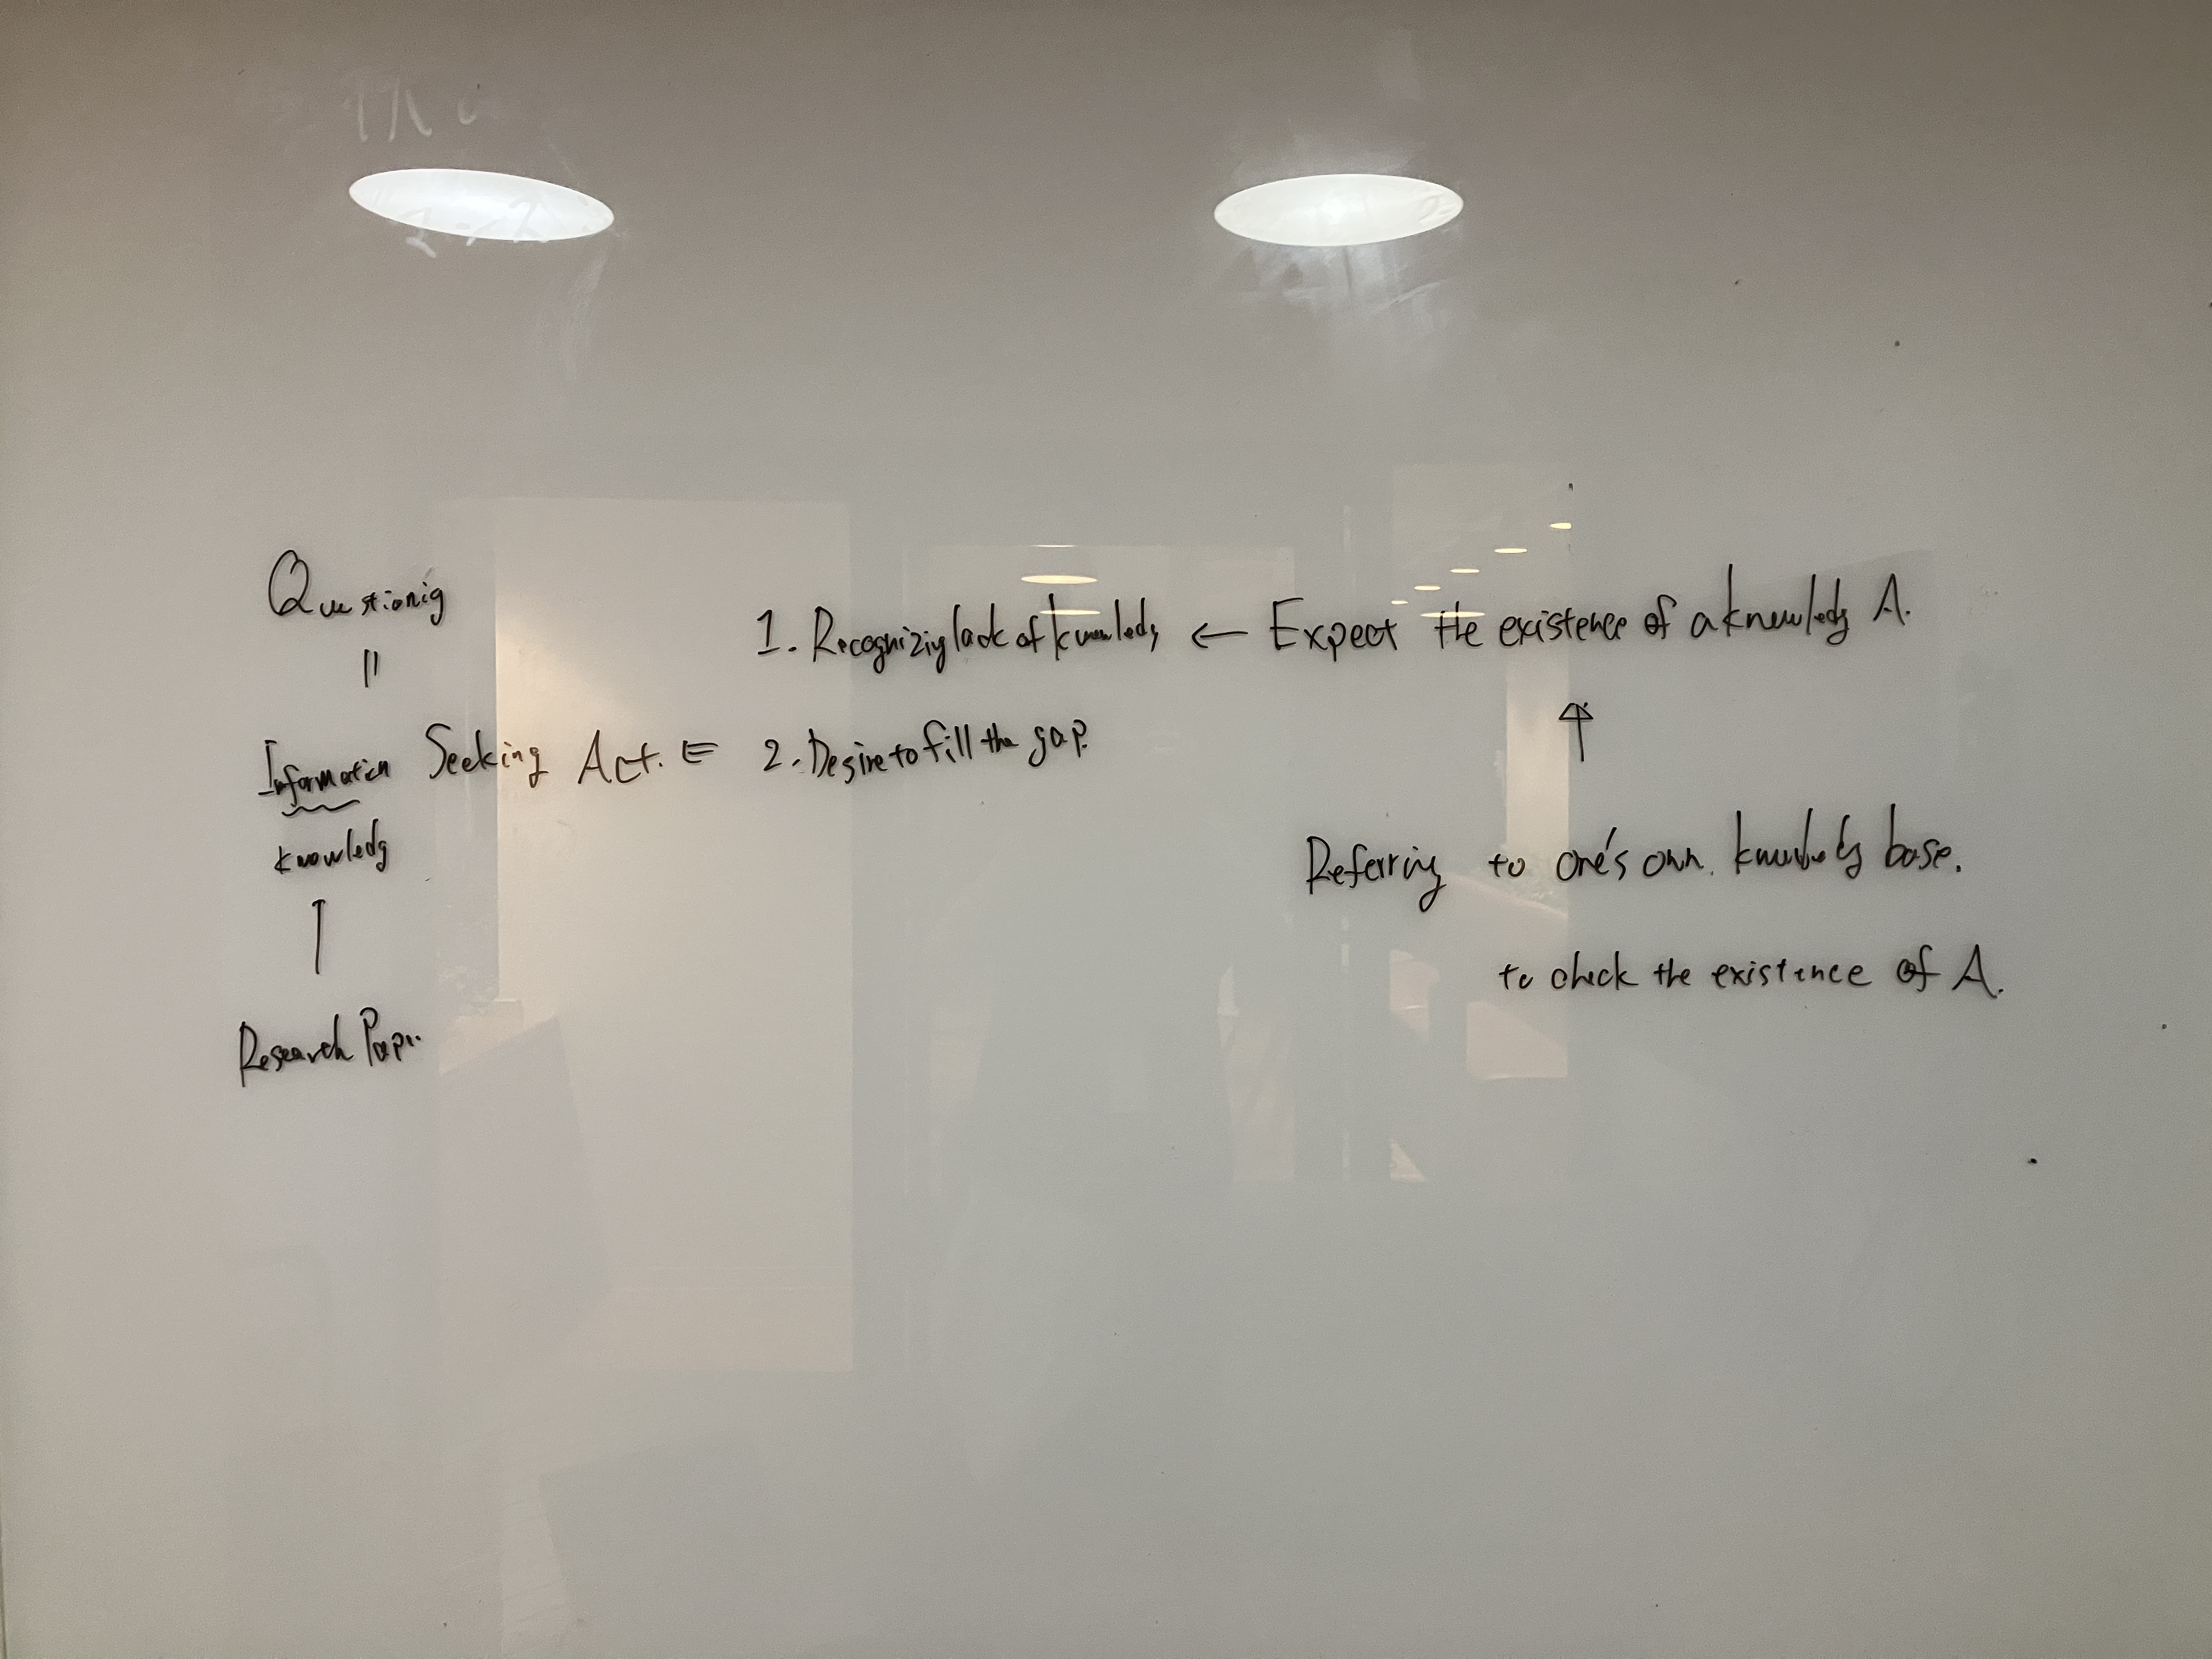
\includegraphics[width=\textwidth]{figs/question_formulation.jpg}
%     \caption{question construction}
%     \label{fig:enter-label}
% \end{figure}

% \textcolor{red}{TODO: Is question construction information retrieval??}


% Asking questions is an act of seeking information \cite{watson2015ask}. The act of seeking information (or knowledge) arises from realizing the lack of one's own knowledge and the desire to fill that gap. Therefore, to create intelligence that can autonomously ask questions, it is necessary to incorporate mechanisms that induce these behaviors.

% Determining what triggers this behavior in humans is a challenging problem. However, when designing a system, it is sufficient if it can induce such behavior, regardless of what it actually is. The principle that ``behavior is triggered when it is somehow desirable for the agent'' represents this idea. You are probably familiar with this concept in reinforcement learning, where rewards (desirability of actions) are provided, and maximizing the expected value of these rewards is formulated as an appropriate way to induce behavior.

% The notion of triggering behavior by realizing the lack of one's own knowledge and attempting to fill it has been extensively studied in the context of curiosity in the field of reinforcement learning. In research, agents that pose questions can generally be formulated within this framework.

% \subsection{question construction}
% The construction of a question is the act of seeking information \cite{watson2015ask}. Specifically, in the context of research, I consider information as knowledge. The act of seeking knowledge involves two steps: 1. Recognizing the lack of knowledge and 2. Attempting to fill that knowledge gap. In this discussion, I assume that intelligence is designed to consistently generate questions when given input. Therefore, I temporarily set aside the aspect of "triggering action" related to the second step of attempting to fill the knowledge gap.

% The recognition of a knowledge gap occurs when I expect to have certain knowledge and, upon referencing my accessible knowledge, I find that it is not available. For example, when running a program and encountering an error that I cannot resolve on my own, I recognize that I lack the necessary knowledge.

% The reasons for expecting the existence of certain knowledge can vary and are arbitrary. In this case, I assume that a purpose given by a third party creates an expectation of certain knowledge. For example, in the case of humans, I first consider what I need to do to achieve a certain purpose. I then anticipate the necessary knowledge to accomplish those tasks, and when I find that it is not present within my existing knowledge, I recognize the knowledge gap.

% Lastly, in this discussion, knowledge refers to the collective body of research findings, particularly academic papers. In actual research, a researcher may personally have a question and then investigate previous studies to confirm that it is indeed unknown before formulating it as a research question. However, what is important in the construction of a research question is that it is unknown to other entities. Therefore, for simplicity, I directly refer to the entirety of academic papers without including the step of comparing personal knowledge.

% To summarize, to create an intelligence capable of constructing questions in this setting, I need to design it to expect the necessary knowledge to achieve a given purpose provided by a third party, search for that knowledge in academic papers, assess whether the papers contain sufficient knowledge to achieve the purpose, and express any knowledge gaps as questions.

% In this case, I excluded the discussion of triggering action by design. However, when considering increasing autonomy, it is important to discuss how to incorporate this aspect into learning and acquisition. The question of "why do I seek information" has been extensively discussed in the context of curiosity.

% Furthermore, in this case, I defined the expectation of knowledge as aiming to achieve a given purpose. However, as mentioned earlier, this does not affect the formulation of questions. For example, let's consider the case of a child asking, ``Why is the sky blue?'' In this case, the child may already have prior knowledge of the concept of ``sky'' and ``blue.'' Additionally, they may possess a naive concept of causality, believing that ``A is B, so there must be a reason for it.'' Thus, they may have expected to have the knowledge that ``the sky is blue because of B.'' However, when they reference their internal knowledge, they find that it does not contain the corresponding knowledge. Therefore, they may have asked the question ``Why is the sky blue?'' to evoke the knowledge they were lacking.

% In this way, the reasons for expecting the existence of certain knowledge can vary, and what, why, and how I seek information (knowledge) are not constrained by specific conditions. Therefore, when attempting to create an intelligence capable of constructing questions in the future, it is feasible to develop a more flexible intelligence.

% Additionally, in this case, I assumed that the given purpose and its achievement are predefined goals. However, humans naturally set their own goals. When considering the design of a more autonomous intelligence, it is conceivable to aim for automation in this aspect as well. However, as mentioned earlier, the question of what I seek knowledge about is not specific to research. Therefore

% , I temporarily set it aside for now. If I were to pursue this direction further, it would ultimately lead to an infinite regress, raising the question of how much information to consider as given.

% \begin{figure}[htb]
%     \centering
%     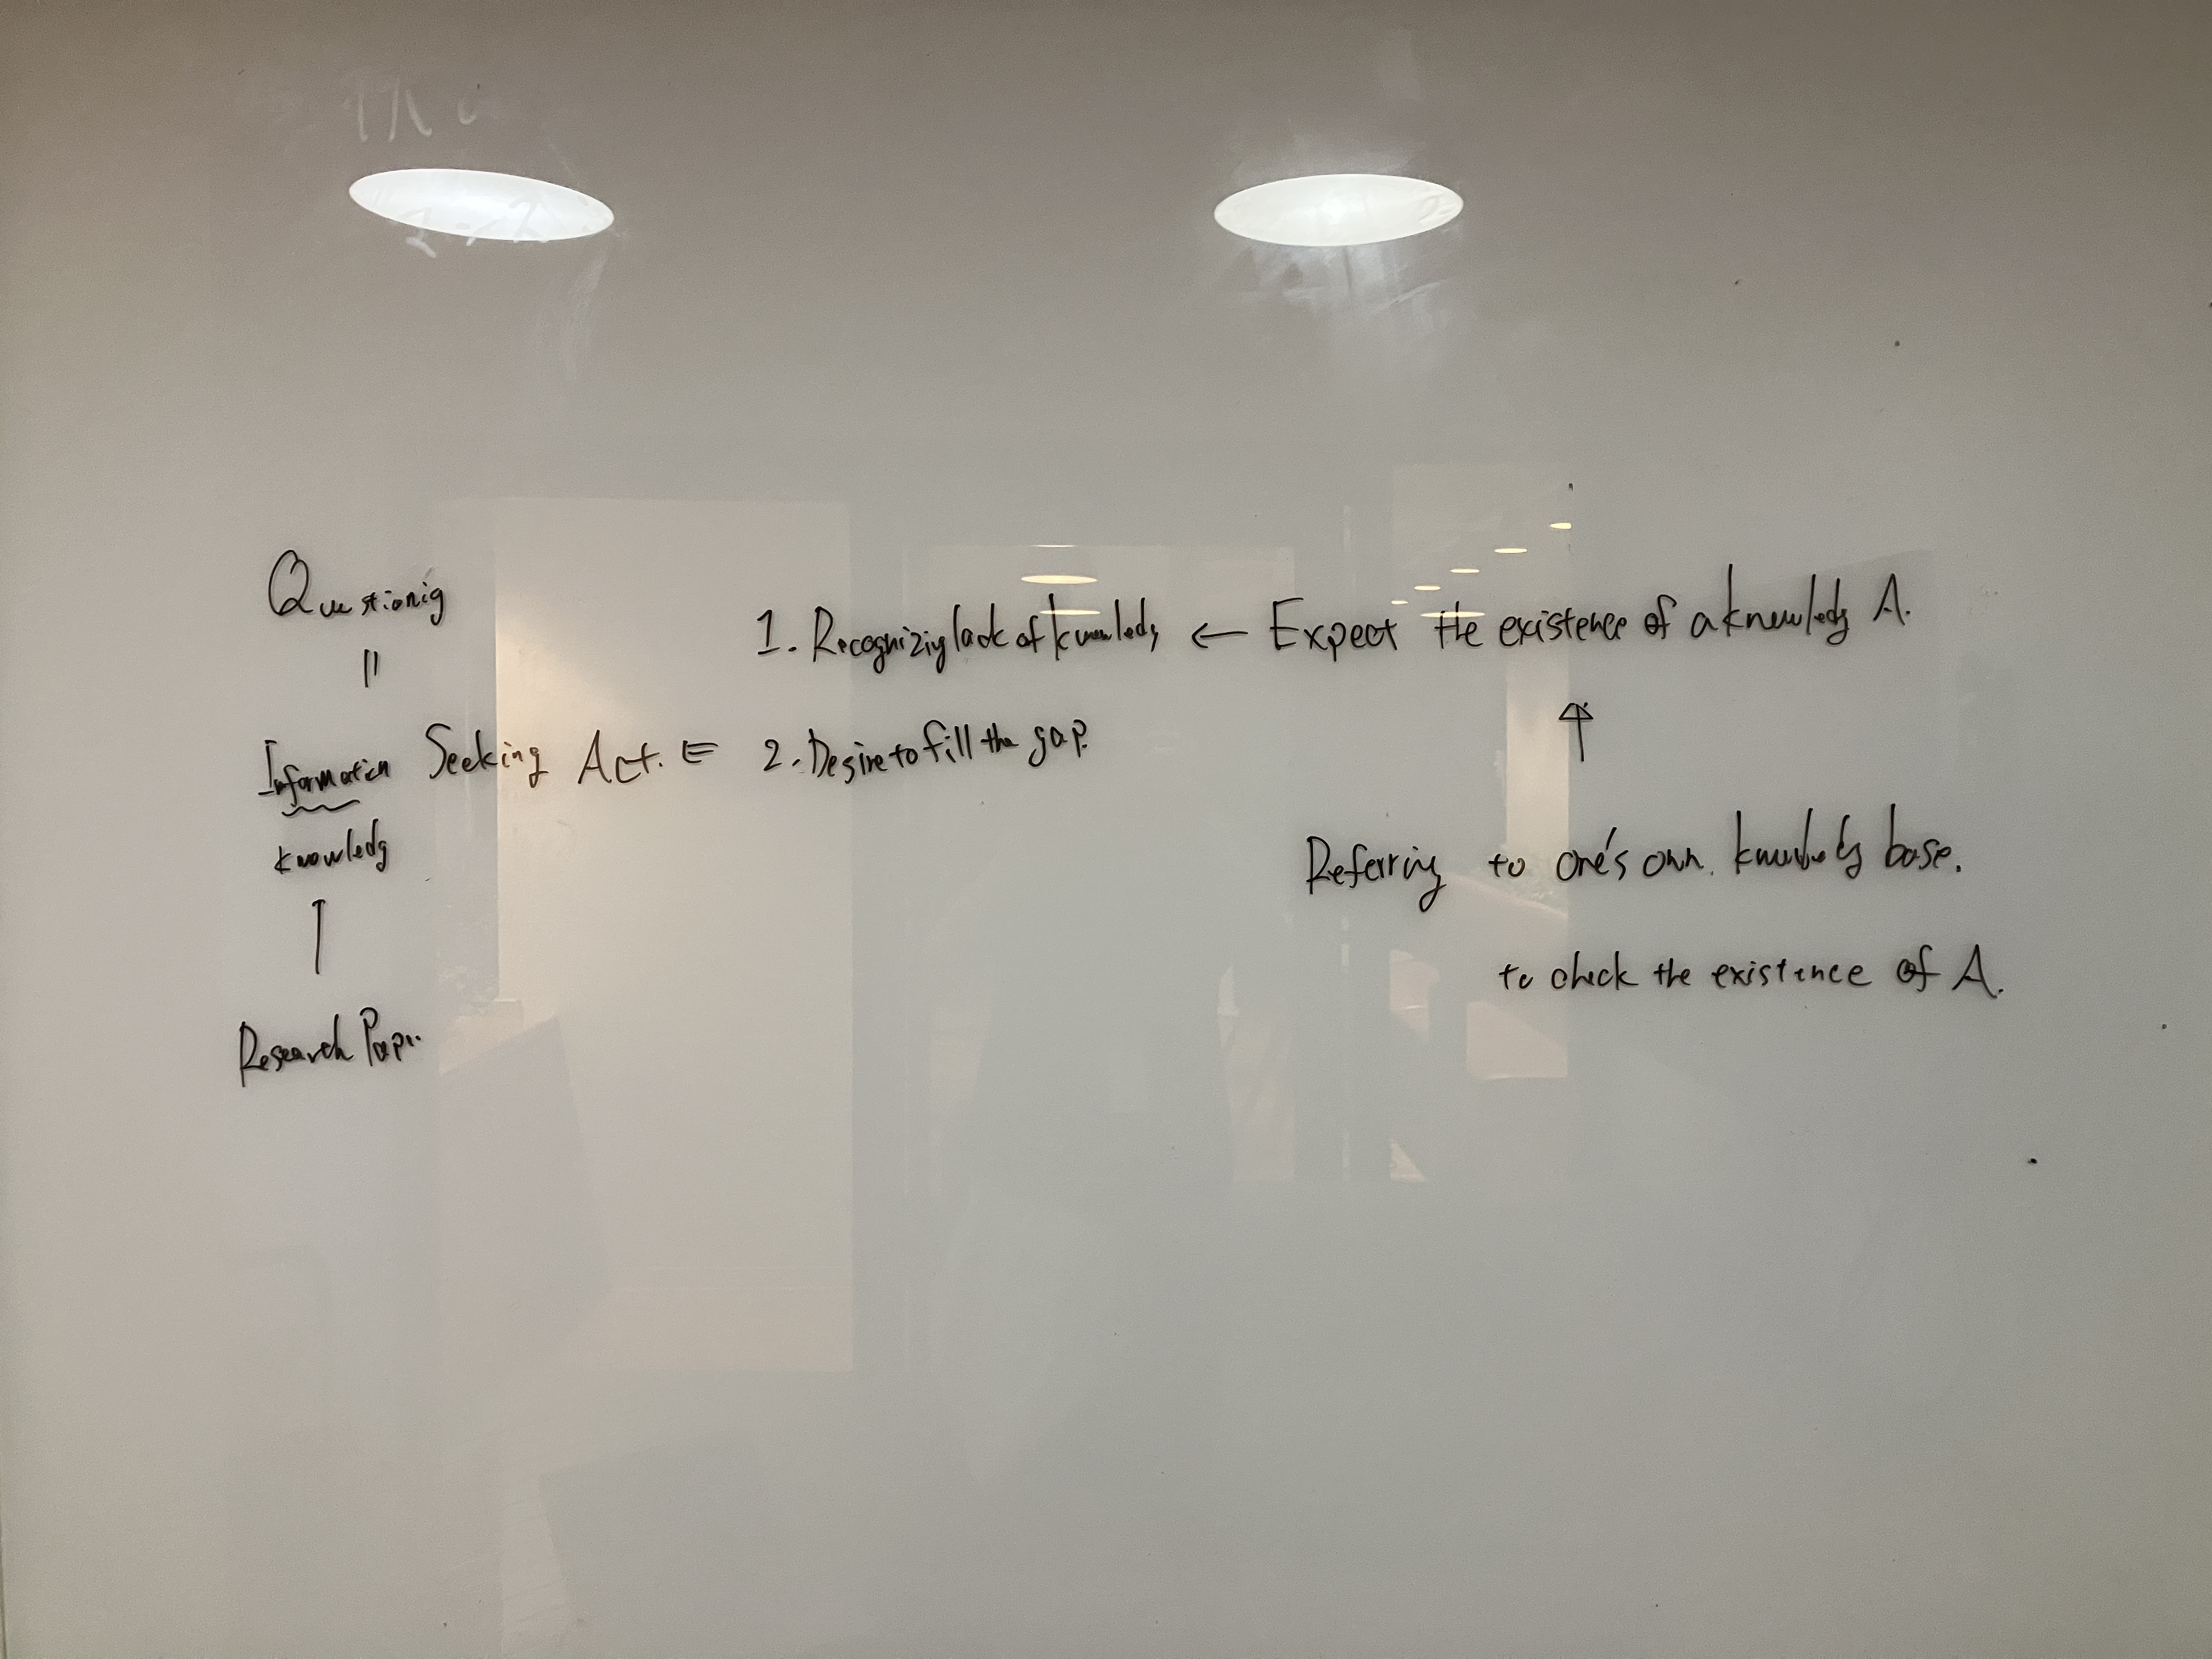
\includegraphics[width=\textwidth]{figs/question_formulation.jpg}
%     \caption{question construction}
%     \label{fig:enter-label}
% \end{figure}


% \textcolor{red}{TODO: Is question construction information retrieval??}


% \subsection{Conclusion}

% \begin{enumerate}
%     \item Determing the existence of expected knowledge:
%     \begin{enumerate}
%         \item Searching for knowledge directly related to the expected knowledge.
%         \item Determining whether the knowledge has been properly validated.
%     \end{enumerate}
% \end{enumerate}

% 1.b is specific to the automation of research. 





% I have listed what I believe are important elements in the construction of questions. However, these are considered important under the assumptions mentioned earlier. For instance, if the goal is not to acquire knowledge necessary for achieving an objective, but to generate knowledge that an individual finds interesting, the necessary elements in question construction (particularly in parts 1.a and 1.b) would change. As previously mentioned, the value of knowledge is determined in relation to context and there's a high degree of uncertainty about how the value of knowledge will evolve in the future. This makes it fundamentally important to have a diverse range of ways to generate questions. The object achievement is highly prevalent and is expected to produce ``important'' knowledge, which is why it is discussed here. However, it is important to discuss what other ways of formulating questions could exist and how they can be implemented.

% \subsubsection{Challenges}
% The first issue discussed in Chapter 2 is the problem of determining the unknown nature of the answer to a question. Given that research is an endeavor to produce new knowledge, it is necessary for the answer to the question to be unknown. Therefore, there is a need to generate such questions or later verify that the answer to the question is indeed unknown.

% The second challenge is the issue of how to make a machine generate a ``good'' question. Firstly, what researchers consider as a ``good'' question is not always consistently agreed upon among them. Furthermore, we pointed out that the ``goodness'' of a question is inherently a concept relative to the individual or society. Hence, there seems to be a need to clearly define what constitutes a good question and think about how to effectively integrate these definitions.

% The third challenge is that as we demand more autonomy from AI, the automation of question formulation becomes more difficult. Inherently, questions are constructed based on various motivations, such as pure intellectual curiosity or for specific objectives. It is very challenging to automate the construction of questions without defining which of these motivations should be the source. Moreover, as mentioned in Chapter 2, the construction of questions encounters the problem of infinite regression when pursued with strict autonomy. Even if not taken to that extreme, setting higher-order objectives behind questions for AI is an exceptionally difficult task.

% It seems that the automation of question formulation has received relatively less attention compared to other processes. Since the formulation of questions is an essential element in conducting research, it would be desirable for more focus to be directed towards the research on automating this process.

\subsection{Hypothesis Generation}
より良い推論ができるようになるには、という話で、結局汎用人工知能を作りたいというかなり広い論点と被ってしまう、という注意を入れる
より良い人工知能を作りたい多くの人が関心がある論点。科学研究にユニークな点としては、探索空間が広大であることなどが知られてる。仮説空間を陽に定めない場合は、自分自身も知らないという状況がユニーク。これを解決するためにつような要素は結局みんなが必要だと思ってる要素だけど、みたいな話。

The second component is \textit{hypothesis generation}. Research is the endeavor to find answers to research questions. Here, as mentioned before, these questions are ones for which the answers are not known. Therefore, we generate hypotheses as candidate answers to these questions and find answers by validating them. Given that research is an endeavor to turn the unknown into the known, the generation of hypotheses, whether implicit or explicit, is an inevitable element in research.

% \subsection{What Would be the Challenges for an AI to Generate Hypotheses?}
\subsubsection{Challenges: Hypothesis Generation as Question Answering}
In research, hypothesis generation is question-answering based on existing knowledge. That is to say, generating hypotheses is equal to predicting answers to questions from one's own knowledge base. I believe that, by design, machine learning models generate hypotheses (this is different from the case of question construction and hypothesis verification). This is because machine learning models make predictions based on data. Therefore, I consider the generation of hypotheses in itself not to be the challenge for creating an artificial researcher.

However, the capacity for scientific hypothesis generation by machine learning models seems to remain limited. For exaxmple, there are still no examples where machines have generated hypotheses or theories that fundamentally change science as Newton or Einstein did\footnote{
If humans define the hypothesis space in advance, machines can generate hypotheses that can solve longstanding problems in a field (e.g. AlphaFold \cite{jumper2021highly}).
}. Therefore, it seems that there are still challenges to be solved in order to create AI that can generate hypotheses like humans.

\subsubsection{Challenges: Generating Hypotheses for AI}
The characteristic of hypothesis generation in research is that it involves question-answering that seeks to find answers that nobody in the world yet knows. Bearing this in mind, I believe that one of the significant challenges is to endow AI with the ability to generate reliable answers to questions that even it, including everyone else, does not yet know the answer to.

Even now, machine learning models are being used to generate scientific hypotheses, but it seems that they are referred to as hypotheses in the sense that their predictions are uncertain to humans, which may be unknown to us. This might be trivial for the machine. In other words, what is a hypothesis to humans may not be a hypothesis to the machine. 

Even if hypotheses for humans are successfully generated, the machine may not be able to generate hypotheses effectively for questions whose answers are unknown even to itself. Indeed, it is known that machine learning models can fail to predict accurately under naive distribution shifts \cite{shen2021towards}, and they are also known to fabricate facts about knowledge they do not possess \cite{maynez2020faithfulness}.

% Furthermore, the essence of human hypothesis generation seems to lie in how to generate plausible answers in situations where the answer is not known. On the other hand, machine learning models are known to just fabricate falsehoods when they do not know the answer \cite{maynez2020faithfulness}. In other words, they do not seem to have sufficiently acquired the methodology to reach an answer under circumstances where the answer is not known. Therefore, it seems important to determine how to generate good answers to questions that are unknown even to the machine itself.

% In summary, I believe the challenges are: 1. How to enable the generation of complex hypotheses as humans do, and 2. How to enable the generation of good answers when the answer is unknown to the machine itself. To find leads for solving these challenges, it seems useful to examine how humans generate hypotheses. In the following sections, I will express my personal view on how it is believed that humans generate hypotheses.

% 研究における仮説生成は既存の知識に基づく質問応答です。つまり、自分が持っている知識から、質問に対する答えを予測するのが仮説生成です。

% 機械学習モデルはデータに基づく予測をします。その意味で、機械学習モデルは設計上すでに仮説生成をしていると私は考えています(これは問いの生成や仮説の検証とは大きな違いです)。つまり、仮説を生成させること自体は課題ではないと考えています。

% 一方で、依然として機械学習モデルの科学的な仮説生成能力は限定的であるように思われます。

% 従って、いかにして人間のような複雑な仮説生成ができる AI を作成するか、というのが問題の一つであるように思われます。

% また、人間における仮説生成の本質は、答えがわからない状況でいかに確からしい答えを生成するかという点にあると思われます。他方で、機械学習モデルは自分が知らないことについてはそれを認識できていなかったり、嘘をでっちあげてしまうことが知られています。つまり、答えを知らない状況下で答えに辿り着く方法論を十分に獲得できていなように思われます。したがって、「機械自身にとっても」その答えが未知であるような問いに対して、いかにして良い答えを生成させられるか、というのが重要であるように思われます。

% まとめると、    1. 人間のように複雑な仮説の生成をいかに可能にするか、2. 機械自身にとっても答えが未知であるときにいかに良い答えの生成を可能にするか、が課題であると私は思っています。これらの課題解決への糸口を掴むためには、人間がどのように仮説生成をしているかを見ていくのは有用であるように思われます。そこで、以下のセクションでは人間がどのように仮説生成をしているかを見ていきます。

\subsubsection{How Do Humans Generate Hypotheses?}

In order to create an AI that can generate reliable answers to difficult questions whose answers are unknown to anyone, it seems prudent to look at how humans generate hypotheses. Therefore, I would like to briefly present my thoughts on how humans appear to generate hypotheses. 
Note that the methods humans use to generate hypotheses are diverse, and the discussion here can by no means cover them all. I hope that what I present can be taken as a starting point for further exploration.

% \subsubsection{The Complex Step-by-Step Hypothesis Generation Process}
One significant difference when comparing the hypothesis generation process of humans and the question-answering of machines is that the human hypothesis generation process is far more complex.


It seems that in the process of generating a hypothesis to answer a single question, humans implicitly and explicitly generate dozens or even hundreds of questions and hypotheses. As a result, in order to answer the initial question, they end up answering many different questions. Moreover, in order to generate a hypothesis, they may also test other hypotheses.


For example, Charles Darwin began with the question ``How does evolution occur?'' However, after reading Lyell's work and becoming convinced of the importance of selection in evolution as an analogy of artificial selection, he formulated and tackled the question ``How does selection (equivalent of artificial selection) occur in nature?'' Here we see a shift in the question. It was precisely because of this change in question that, upon reading Malthus's essay on population, he was able to realize that natural selection is brought about by competition between species, and thus he could fully answer the initial question, ``How does evolution occur?'' \cite{gribbin2022origin}

On the other hand, it appears that we are not having our neural networks go through such a complex process of trial and error for hypothesis generation. In many cases, when a question is presented, neural networks predict answers through a single inference based on fixed parameters. This seems too simplistic compared to the human process of hypothesis generation, which often involves repeatedly generating and testing questions and hypotheses.

% For humans, answering a question essentially means constructing the answer from known concepts. A question whose answer is unknown can be said to be one whose answer does not immediately connect with existing knowledge. Humans seem to somehow successfully link the unknown answer with their known knowledge. As these examples also illustrate, realizing the prediction of answers in cases where the answer is unknown to everyone in the world appear to be a challenge.
% 人間の場合、ある問いに答えるとは、その問いの答えを既知の概念で構成することに他なりません。答えがを知らない問いというのは、その答えが既存の知識に直ちには結びつかない問いであると言えます。このような状況下で、なんとかして答えが未知の問いを既知の知識に結びつけるのが、人間が仮説生成をする際に行なっていることであるように思われます。

% \subsubsection{Analyzing Question}
\textcolor{red}{TODO: remove or modify}
In difficult questions where the relationship to known knowledge is not immediately apparent, it seems that we first tend to analyze the question in detail. For example, let's say you have a question, ``Why are apples red?'' The first thing you would consider is what an apple is and what red means. You would also think about what it means for something to be red. Then, you would focus on the properties of apples and the color red and abstract them. you may also think about other red things besides apples. If you already know the reason why tomatoes are red before knowing why apples are red, you might consider that the reason for tomatoes being red could apply to apples as well. By conducting this kind of analysis, you can connect your understanding to existing similar knowledge and attempt to explain using those existing reasons. These ways of focusing on abstract structural similarities between specific concepts and inferring that what can be said about A, which has the same structure, can also be said about B is called \textit{analogical reasoning}. This has been considered to be important method in hypothesis generation \cite{thagard_1984}.

I believe that the process of analyzing a question corresponds to the feature transformation that occurs via the intermediate layers in a neural network. In this sense, neural networks also analyze questions. The difference may lie in the fact that humans explicitly perform the analysis of the question and ultimately make inferences for answers based on formal similarities that are linked to symbolic known knowledge.

% hesse1965models,thagard_1984,gentner1993shift,holyoak1996mental,dunbar1997scientists

% I began by explaining that I first formulate the unknown I am addressing in the form of a question. The process of finding answers to this question is research. Here, because the answer to this question is, of course, unknown, it requires inference as to what the answer could be. As a result of this inference, a plausible answer is formulated. This process corresponds to the \textit{hypothesis generation}. Hypothesis generation is the inference about the unknown and the definition of research is to transform unknown to known. Thus, every research including deductive research must entail hypothesis generation implicitly or explicitly. In this sense, hypothesis generation should be the second module of knowledge production system.

% The belief that a hypothesis is true is the very object that can become knowledge in response to a question. If a hypothesis withstands proper testing, the belief in its plausibility strengthens. Conversely, if a hypothesis does not withstand testing, that belief is weakened. Therefore, the former generates knowledge that ``the answer to question A is hypothesis B,'' while the latter generates knowledge that ``the answer to question A is not hypothesis B.'' 

% Hypothesis generation is the act of creating potential answers to a question, so naturally, it is essential to generate plausible hypotheses that are close to the actual answer. Therefore, let's start by referring to how humans generate hypotheses and then discuss how I can generate reliable hypotheses, drawing inspiration from human methods.

\subsubsection{Types of Questions}
There are various types of questions. For instance, a ``How'' question is posed when one wants to know a specific way to do something, while a ``Why'' question is asked when one is curious about the cause or mechanism of something. Among them, it would not be an exaggeration to say that the ``why'' question is of the highest interest to researchers. Researchers have developed methodologies for expressing queries about causality and for inductively inferring answers to those queries based on them, i.e.\textit{ causal inference} \cite{pearl2018book}.

An AI tasked with formulating questions autonomously is expected to be capable of posing questions, regardless of their question type, and to develop methodologies for answering them. The broader the class of questions that need to be addressed, the more general the methodology required becomes. How to realize such an AI remains an open question.

\subsubsection{Challenges}
One challenge in creating an intelligence capable of hypothesis generation, not just as a tool for humans, is the need to empower the machine itself to form plausible hypotheses for questions to which even the machine doesn't know the answer. Current machine learning models have been criticized for potentially not knowing what they don't know \footnote{
In our discussion with Wataru Kumagai, we were reminded once again of the importance of self-awareness in creating an AI capable of conducting research.
}. 
Moreover, they are known to confidently provide answers or fabricate falsehoods about topics they are ignorant of. Therefore, it seems essential to first accurately recognize what is unknown, either for oneself or the world at large, as told in sections of question construction. Upon facing an unknown subject, there's a need to reduce uncertainty and approach understanding. As mentioned in Chapter 2, humans attempt to understand uncertain subjects by gathering information from papers, experiments, or by reframing questions. While it may not be necessary to adopt the exact same approach, it seems essential to enable machines to autonomously adopt strategies to reduce uncertainties.

% Outputs from machine learning models are essentially inferences tinged with uncertainty. From this perspective, one could posit that these models are already inherently generating hypotheses. Indeed, they are already employed for hypothesis generation in numerous scientific investigations.

% However, while these hypotheses might be hypotheses in the sense that the answers are unknown to humans, they might be self-evident to the machine learning model. When we talk about AI generating hypotheses in the context of AI conducting research, the ultimate expectation is for the AI to provide plausible answers to what is unknown to AI itself. This remains an unresolved issue.

As one of the promising approaches for tacking unknowns, it seems crucial for AI to acquire systematic thinking to realize this, as humans developed systems like language and mathematics, allowing them to infer about subjects beyond their experience. Systematic thinking is not only important for out-of-distribution generalization but is also valued for interpretability, causal inference, logical reasoning, mathematical processing, and planning.

% \textcolor{red}{TODO}

\subsubsection{Others}
Theoretical virtues \cite{schindler2022theoretical}

GPT-3 learn to quantify the uncertinty of its answer \cite{lin2022teaching}

LLMs know that they know \cite{kadavath2022language}
 
can ChatGPT generate scientific hypothesis? \cite{park2023can}

\subsection{Hypothesis Verification}
The third sub-module is hypothesis verification. Knowledge production in this paper is defined as the process of justifying beliefs in a way that convinces members of the society. Hypothesis verification corresponds to this justification. As explained in Section \ref{section-knowledge-production-as-belief-revision}, I believe that science is a reliable source of knowledge production precisely because it is grounded in methods based on strong beliefs that are held by virtually every human being and are so fundamental that even everyday life would be impossible without them.

In the previous section, I pointed out the possibility that allowing verification methods to be entirely autonomously constructed could result in outputs that are meaningless to humans. So, what exactly needs to be created, and to what extent, in order to develop an AI capable of performing verification? I would like to consider this point in this section.

I consider the notion of verification as an update of shared beliefs to be useful in comprehensively describing the process of verification across a wide range of research, from theoretical studies to humanities. However, it might be somewhat too abstract when aiming for the current purpose. To provide a foundation for further discussion, I would like to focus on verification in science, particularly on its core elements: experimentation and statistical analysis.

\subsubsection{Experimentation}
Experiments are generally considered a series of procedures to test a hypothesis, particularly referring to the process of data generation. I believe that the main elements in an experiment are the interventions to test a hypothesis and the generation of data to artificially create observations of phenomena. Verification is then done through the analysis of data obtained from these experiments.

The experiment can largely be divided into three phases: designing the verification plan, preparing to execute the verification plan, and actually carrying it out. Therefore, it seems that in order to create an AI that can conduct experiments, we must create an AI capable of performing all of these tasks.

% \subsubsection{Automating Experimentation}
実験の自動化のレビューの話を書く、LAとか実験計画とか

% \subsubsection{Understanding Verification}
To become capable of designing verification plans, it seems necessary to have the ability to understand what verification is and the ability to engage in long-term planning. Additionally, preparing for verification, possessing a human-like body, and the capability to manipulate it freely will be required. Among these, the acquisition of intricate planning and flexible action has been the subject of research by many artificial intelligence researchers.

On the other hand, the acquisition of the ability to understand verification seems to receive relatively little attention. There are indeed studies that focus on the importance of verification for reducing hallucinations and verifying the reliability of scientific claims, but these do not aim to determine what constitutes verification in scientific research. Therefore, I believe that considering how to make machines comprehend what can qualify as verification remains one of the challenges ahead.

\subsubsection{Statistical Inference and Verification}
In science, the validity of hypotheses is judged based on data generated from experiments using inductive reasoning. We have formalized inductive reasoning with concepts from probability theory and constructed methods to perform inductive reasoning through statistical inference. Inductive reasoning is a premise of science, and implementing it via statistical inference is a widely practiced approach. Therefore, when creating an AI capable of performing meaningful verification for humans, it would be sensible to take these as a given (this relates to the points mentioned earlier).

On the other hand, there can be multiple interpretations of what it means for a hypothesis to be justified by statistical analysis \cite{otsuka2022thinking}. This implies that there are conflicting views on what methodology should be adopted to justify beliefs. As a result, there are multiple methodologies for statistical inference. Ideally, a machine capable of verification should understand ``why a certain inference is valid in justifying a hypothesis''  and be able to select or construct an appropriate methodology from these options. Otherwise, it might not truly understand what constitutes verification.

To create an AI that can verify hypotheses, I believe it is necessary for the AI to understand the basis for verification. However, to create an AI that can perform human-like science, it may be sufficient if it can appropriately use statistical inference methods, which humans employ. This is because even if it doesn't understand why that constitutes verification, as long as it uses statistical inference correctly without violating its premises or rules, there should be no issue in using it just as a tool. In reality, even humans do not always seem to grasp these differences when conducting verification. For instance, it is not uncommon for people to use hypothesis testing without understanding why it is a valid means of justifying beliefs about a hypothesis. 
% 科学では、実験で生成したデータをもとに帰納推論によって仮説の妥当性を判断する。私たちは帰納的推論を確率論の概念で定式化し、統計的推論によって帰納推論をする方法を構築してきた。帰納推論をすることは科学の前提であり、統計的推測によって帰納推論を実施することは広く行われている実践である。したがって、人間にとって意味のあるような検証ができる AI を作る際には、これらは所与のものとするのが良いだろう(これは上で述べた論点と関連する)。

% これに対して、統計的分析によって仮説が正当化されるとはどのようなことなのかについては複数の解釈が存在しうる。これはすなわち、信念を正当化するためにはどのような方法論を取るべきかという点について対立する立場があることを意味する。その結果、複数の統計的推論の方法論が存在している。したがって、理想的には検証ができる機械は、「なぜその推論が仮説を正当化する上で妥当なのか」を自ら理解し、これらのうちから適切な方法論を選択する、ないし自ら適切な方法論を構成することが望ましい。むしろそれができていないと本当の意味で何を持って検証としているかを理解しているといえないということもできるかもしれない。

% ただし、人間が開発した仮説検定などの統計的推論の手法を道具として適切に使うことができる AI を実現することができれば十分かもしれない。なぜなら、人間でさえこれらの違いを把握して検証を実行している場合は多くないように思われるからである。例えば仮説検定がなぜ仮説に対する信念を正当化する手段として妥当なのかを理解せず、使っている場合も少なくないように思われる。そしてこれは仮設検定という道具を使うための前提や規則に反していない限りでは問題はない。

% As emphasized repeatedly, hypothesis verification in research aims to reduce a belief about the truth or falsity of a hypothesis to a strong conviction. In particular, science has been able to convince many people by reducing their belief about it to such a strong conviction that I can no longer live without assuming it.

% I consider verification to be a particularly crucial process in the generation of knowledge. Questions and hypotheses can be generated in arbitrary ways, and they can take any form. However, verification must not be taken like this. Verification must be done in a manner that can convincingly update the shared beliefs of other members of society. Therefore, it is the most demanding process in the research journey in terms of rigor and caution. I believe that the rigor of this process is what truly sets research apart from other activities. The rigor and systematicity of the verification process is considered the very reason why science or research is referred to as rigorous \cite{sep-scientific-method,hoyningen2008systematicity,haack2003defending}.

% \subsubsection{The Difficulty of Autonomous Acquisition of Hypothesis Verification}
In the case of hypothesis testing, just like in hypothesis generation, the tasks for automating hypothesis testing vary depending on who the hypothesis testing is for. If artificial intelligence is used as a tool for human research, it is sufficient for artificial intelligence to faithfully reproduce what humans do as verification. For example, it would be great if it could conduct, for instance, hypothesis testing. If the machine is capable of automatically preparing for statistical hypothesis testing, calling the appropriate statistical hypothesis testing libraries at the right timing, and using them correctly for the relevant subjects, then I would have no complaints about their performance.

In this case, it is not necessary for the machine to strictly know why it constitutes verification, as long as it can learn from numerous examples of human verification and use it appropriately. In other words, in this case, the required understanding can be described as indirect and practical understanding through examples of human usage. Furthermore, if it can be confirmed that the machine not only mimics humans by using libraries but also understands what statistical hypothesis testing is and its principles, this would be a significant advancement in the automation of hypothesis testing. 

I used statistical hypothesis testing as an example, but the same applies to other verification methods as well. The point is that in this scenario, I seek to enable artificial intelligence to appropriately utilize the verification techniques employed by humans. However, it is essential to note that the verification itself remains relevant and meaningful to humans.

On the other hand, aiming to make machines understand and acquire the concept of verification autonomously from their own perspective becomes an immensely challenging task. This is because, as repeatedly emphasized, hypothesis verification involves the updating of beliefs, and the belief system of machines can significantly differ from that of humans. It doesn't seem that machines can acquire the concept of their own verification just by observing examples of human verification. Furthermore, as explained earlier, machines have not evolved their belief systems through interaction with the natural world. Therefore, verification methods entirely composed and developed by machines may no longer serve as effective tools for understanding nature. How to enable machines to autonomously acquire verification principles from the ground up, address the alignment issues between machines and humans, and ensure that these efforts lead to a better understanding of nature are challenges that the entire community should discuss and explore in the future.
% \subsubsection{Verification and Alignment}

% As I have explained repeatedly, research is the act of updating beliefs by reducing them to a common conviction that satisfies most members of society. Verification is precisely the act that carries out this belief update. Therefore, when considering knowledge production by agents that are not limited to humans, it is an important issue whether to completely rely on the criteria autonomously generated by the agent's society, including the act of verification. This is because what may lead to belief updates for a certain artificial intelligence group may not be the same for humans. In such a case, the knowledge produced there would be completely detached from humans. Therefore, when I want non-human intelligence to produce knowledge that is meaningful to humans, at least the criteria of verification should include elements that humans can agree with.

% Furthermore, as mentioned earlier, the reason why verification, even as the update of collective beliefs, has brought about such progress and benefits to the human society may be because the subject of research is (in a broad sense) nature and because human beliefs themselves are inherently constrained by nature. When I say that human beliefs are constrained by nature, as explained in the section on induction, it means that what I strongly feel to be certain is a reaction to what I have been exposed to through the process of evolution and development as organisms, interacting with nature.

% Considering this, when a fully autonomous artificial researcher is created, I think it is far from obvious whether they would autonomously conduct meaningful research on nature or be able to share knowledge with us humans without possessing at least these naturally constrained intuitions, sensory organs, and basis of beliefs. Therefore, when creating autonomous artificial researchers, it may be necessary to provide them with such nature-rooted beliefs in the form of some inductive bias.

% \subsection{Towards Autonomous Verification}

% As mentioned above, I believe that the process of verification is highly diverse. This diversity makes achieving an end-to-end approach immediately difficult. Therefore, it would be better to start by further breaking down the process of hypothesis verfication into more detailed sub-processes. For a practical first step for the verification process automation, I propose tentatively dividing the verification process into three stages: \textit{verification design}, \textit{verification instantiation}, and \textit{verification execution}. At each stage, you will create a verification plan, prepare for the verification, and carry out the verification.

% \begin{figure}[htb]
%     \centering
%     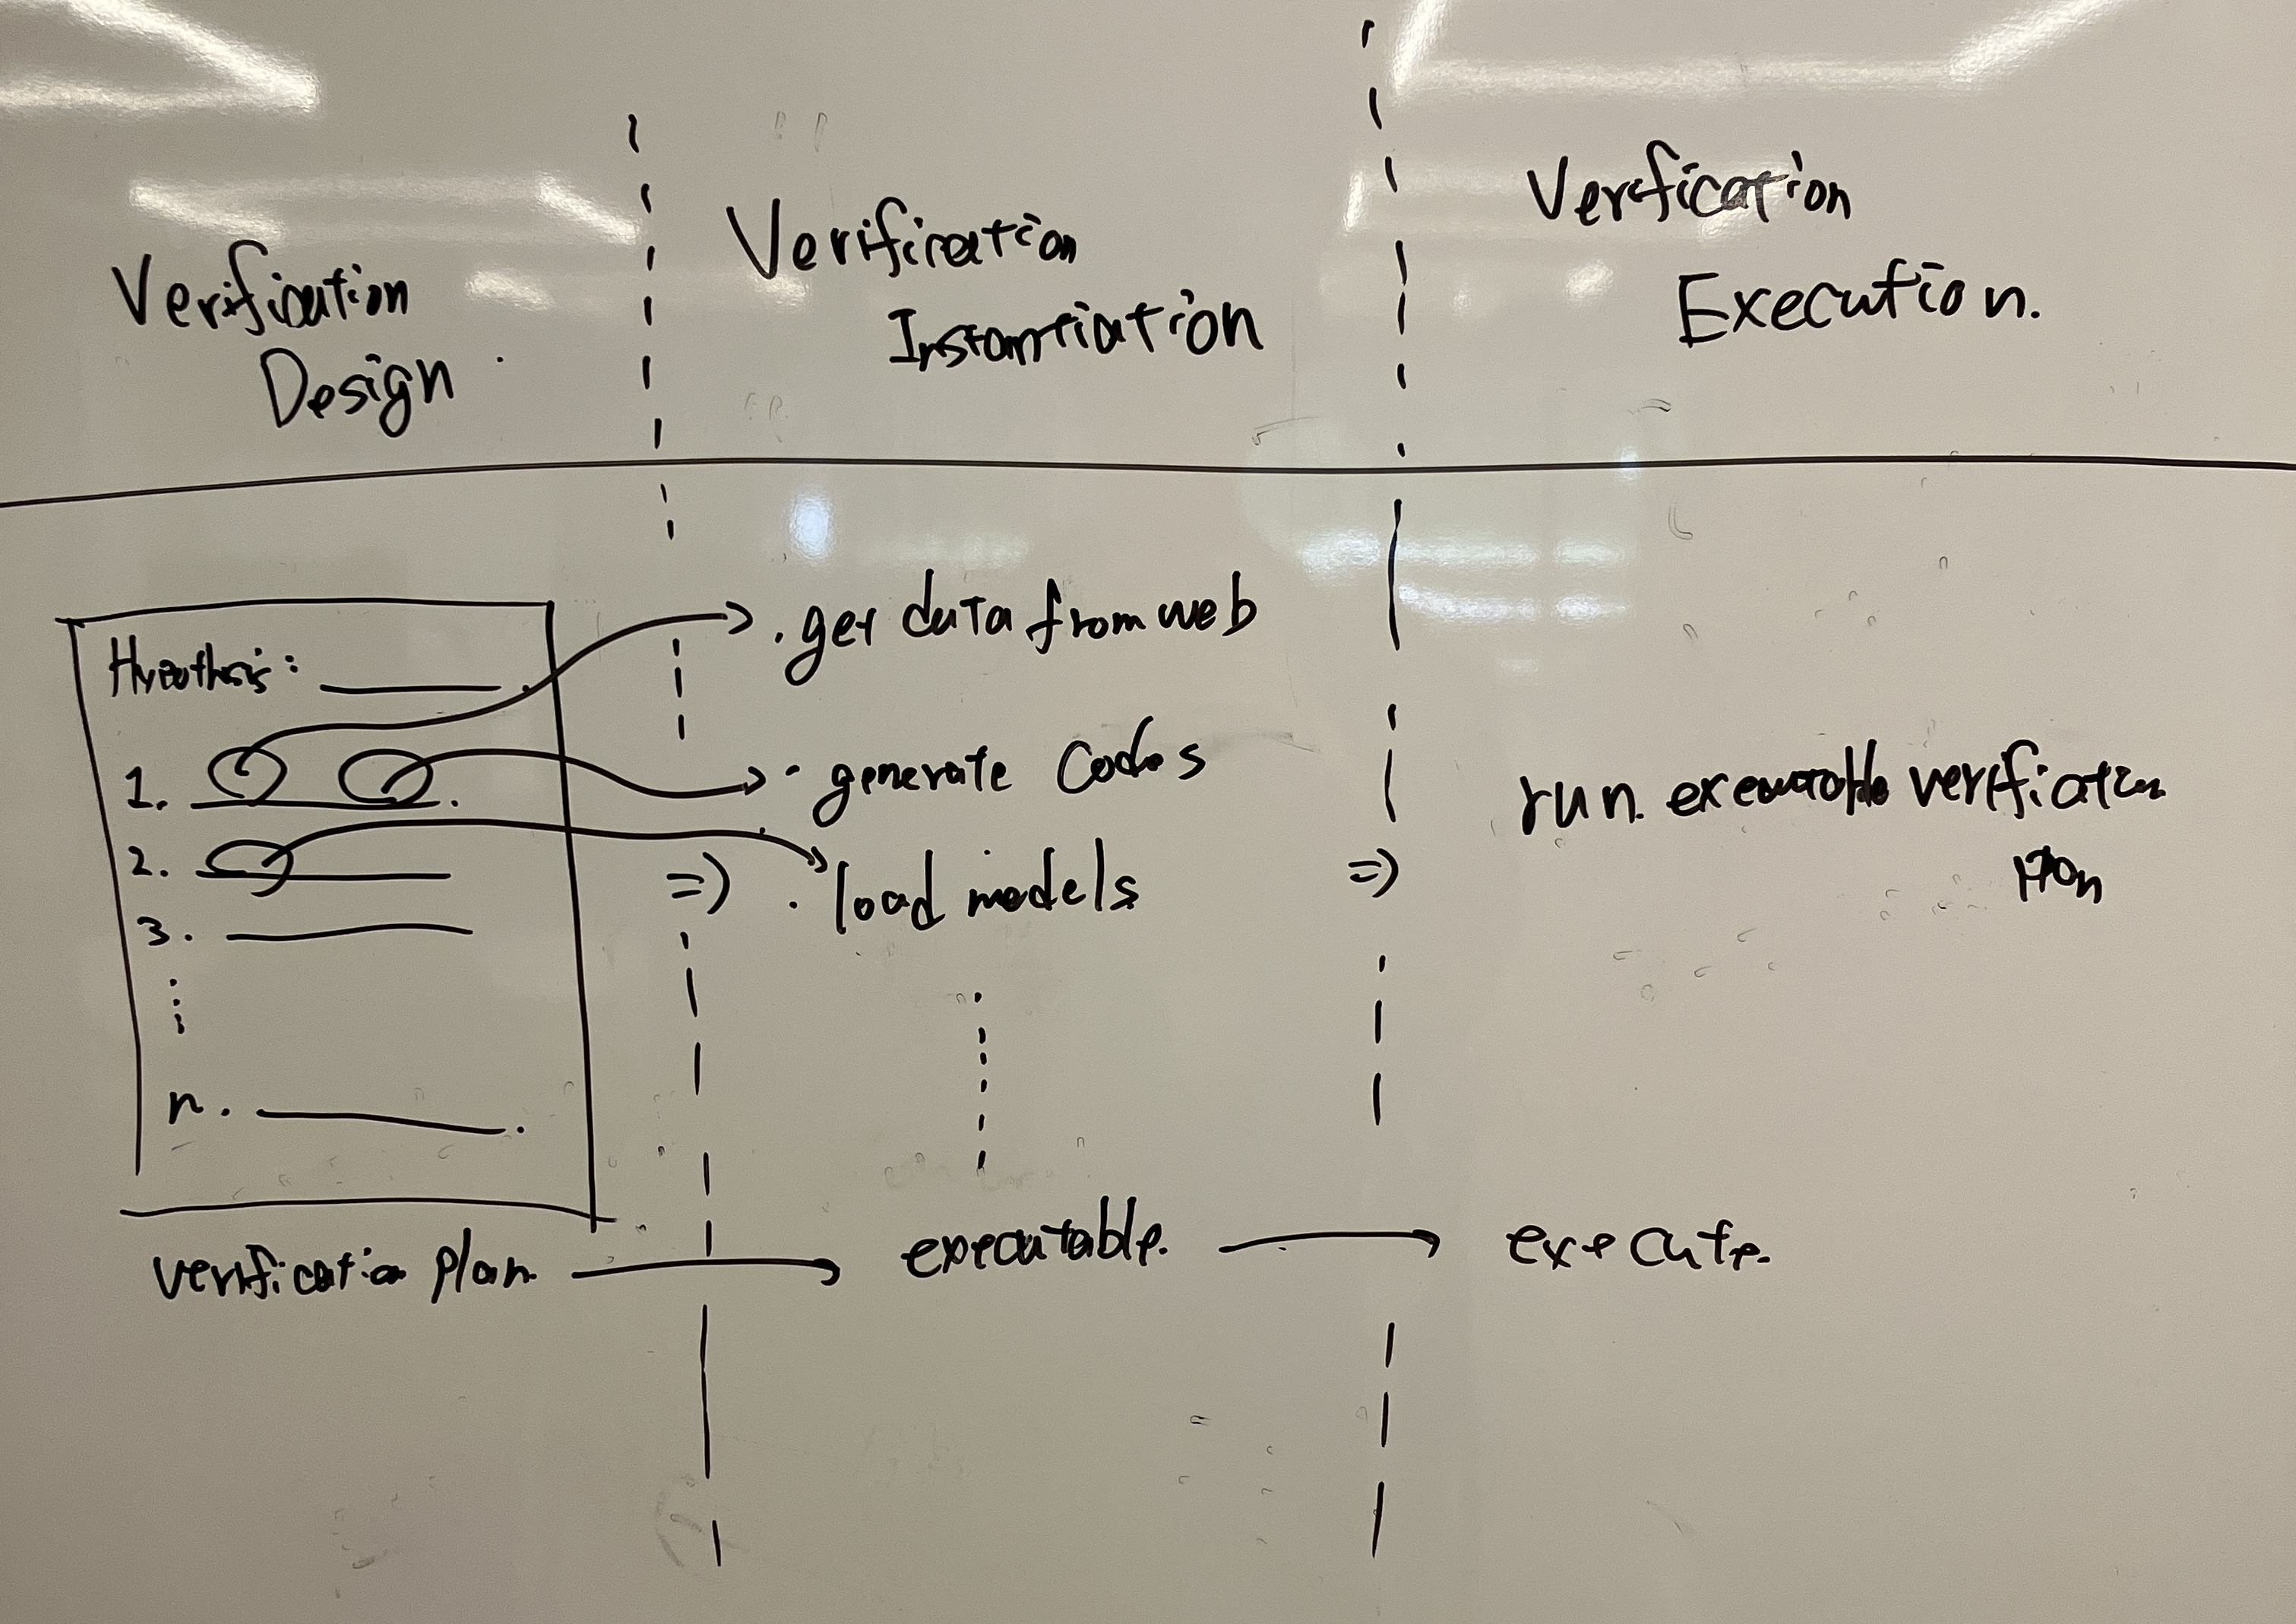
\includegraphics[width=\textwidth]{figs/verification.jpg}
%     \caption{Verification}
%     \label{fig:verification}
% \end{figure}

% \subsubsection{Verification Design} 
% In verification design, the agent will create a plan to execute the verification, which consists of hypotheses, verification criteria (criteria to determine if the output confirms or refutes the hypotheses), and the procedures for conducting the verification. The verification plan should be specific and detailed enough so that anyone faithfully executing it can reproduce the same verification process and result. For example, suppose I am considering an experiment to compare a proposed method with a baseline and validate the hypothesis that the proposed method performs better. In this case, the plan should describe in detail which model to use, what dataset to employ, and how to measure the performance. Thanks to this specification, I can separates the two functionally distinct stages of verification: the phase of considering what needs to be validated and the phase of actually executing the verification.

% It is during the verification design stage that specific skills for hypothesis verification are required. This is because automating the preparation and execution of a plan involves the automation of more general intellectual tasks, not limited to research automation, while creating a verification plan demands an explicit understanding of what verification entails and what criteria constitute a successful verification. In aiming to automate this verification plan, the key lies in teaching machines how to understand the concept of verification.\footnote{
% Even humans may sometimes do verification without proper understanding of the method. For example, someone may conduct hypothesis testing just because ``everyone does it.'' While this may be an extreme example, it is not common for researchers to understand the epistemological implications of inductive reasoning and statistical inference and in what sense I can say I verify a hypothesis. In that sense, the requirement for machines to understand verification may be somewhat challenging. However, if the aim is to truly enable AI to autonomously conduct research, it appears crucial for the AI to have a proper understanding of what constitutes verification.
% }

% % Multiple abilities are needed to create a verification plan, but based on the discussion so far, it is evident that at least two abilities are required.


% % At this stage, I contemplate how to validate the hypotheses and proceed to formulate a verification plan. In a verification plan, the agent writes about the hypotheses, verification criteria (what will be considered as evidence for verification), and the procedures for conducting the verification. These plans should be as much detailed as possible. The Fig. provides an example in the context of machine learning. The idea is to create a blueprint for a pipeline where verification is automatically executed by faithfully following the plan.

% % Furthermore, for artificial intelligence to perform autonomous verification, it seems essential that the AI not only adopts certain verification criteria but also be able to explain the meaning behind them and how they contribute to the verification process. Even humans may sometimes engage in this without conscious awareness, such as conducting hypothesis testing because ``everyone does it.'' In that sense, this requirement may be somewhat challenging. However, if the aim is to truly enable AI to autonomously conduct research, it appears crucial for the AI to have a proper understanding of what constitutes verification and be able to design it itself or, at the very least, explain it adequately.

% There are several abilities that a machine must possess in the context of verification planning, but based on the discussion so far, it is evident that at least two abilities are required: understanding what verification is and planning to achieve objectives.

% Let's first discuss the ability to understand verification. As mentioned in the sections on question construction and hypothesis generation, this is an extremely crucial ability in the overall automation of the research process. As before, the extent to which ``understanding'' is required depends on how much autonomy is expected in the automation of verification. If that is used as a verification tool for humans, what machines to do is just using human verification methods properly. On the other hand, if they were required to understand the concept of verification from scratch, I would face a lot of challenges as I just described in this chapter. 

% If you aim to achieve the former, one of the initial steps could be creating a dataset specifically tailored for verification. By gathering research papers that utilize widely used verification methods like statistical hypothesis testing, you can train a model to construct verification methods from these hypotheses. One naive approach could be to start by generating method descriptions in research papers from the given hypotheses. 

% If you were to achieve the latter, you might want to begin by contemplating what beliefs mean for machines. Alternatively, placing agents in situations where verification becomes necessary could implicitly help them acquire the concept of verification. In this case, addressing the issue of generalization across environments, such as enabling machines to explicitly reuse the concept of verification, will be crucial. Eventually, as repeatedly emphasized, discussing how to resolve the alignment problem will be necessary.

% % If artificial intelligence is used as a tool for human research, it is sufficient for artificial intelligence to faithfully reproduce what humans do as verification. For example, it would be great if it could use basic concepts such as hypothesis testing, controlled experiments, and interventions and automatically create experimental plans based on them. In this case, it is not necessary for the machine to strictly know why it constitutes verification, as long as it can learn from numerous examples of human verification and use it appropriately. In other words, in this case, the required understanding can be described as indirect and practical understanding through examples of human usage. Furthermore, if it can understand the concepts of hypothesis testing and controlled experiments from first principles, it would be a significant achievement in terms of automatic verification.

% % On the other hand, if artificial intelligence itself is allowed to conduct research for its own knowledge generation, it seems that artificial intelligence needs to understand what verification is, whether explicitly or implicitly. And similar to the unknown nature of the answer to a problem, it seems to be an ability that cannot be acquired just by observing examples of human verification. This is because verification involves updating the beliefs of the members of a society, which depends on the nature of the beliefs of the machine group itself. Whether the knowledge generated by such agents is understandable by humans or can say something about nature is not obvious, but this will be discussed in detail in later chapters.

% Let us move on the second ability: planning. Understanding verification is a necessary condition for setting verification criteria by considering what can be tested against a given hypothesis. When conducting actual verification, under the assumption of a hypothesis and verification criteria, one must devise procedures for carrying out the verification. For example, in experimental research, let's say a hypothesis A is formulated, and a verification criterion is established that considers the hypothesis valid if it meets certain criteria through statistical hypothesis testing. To actually perform this verification, it is necessary to generate data to be used for verification, and if there is no apparatus to generate the data, one may need to create it. Thus, in a verification plan, one must develop a plan to fulfill the purpose of executing the verification.

% Creating a plan is known to be a challenging task, not limited to verification plans. To achieve a goal, one must understand what is necessary and comprehend the appropriate sequence of steps to achieve the goal. As mentioned earlier in the section on constructing questions, when creating a plan, it is essential to consider feasibility, taking into account the complex external factors such as current financial capabilities and accessible resources. Understanding and incorporating these constraints appropriately can be a highly challenging task, as they are intricately linked to various external factors.

% While there are already a difficult task, the particular challenge in creating verification plans for research lies in the fact that one may need to create things necessary for verification if they do not already exist. This is an extremely high-level difficulty problem. To carry this out, one must first accurately identify what is currently lacking. After recognizing the deficiencies, one must consider how to create what does not exist. Once the method is known, materials for creating it must be prepared, and it must be actually built. And even if it is created, one must investigate whether they function properly. This is an unbelievably complex task, and it seems highly unlikely to simultaneously expect the creation of such intermediate products by directly generating a verification plan from the verification itself. Therefore, in aiming for true automation of verification, it is crucial to seriously consider how to solve this problem.


% Finally, once the necessary elements for verification are understood, they need to be represented as something that can be understood by other researchers. This is not a requirement of a verification plan but a necessary condition for knowledge to become knowledge for society. In order to generate knowledge for society, it is necessary not only to verify hypotheses but also for the verification procedures to be understandable to other members of society and judged as valid.\footnote{
% While it is desirable for the question generation process and hypothesis generation process to be publicly available, it is of utmost importance that the verification process is disclosed. 
% } Also, as discussed in the section on hypothesis generation, verification must ensure that the causes behind the verification results are traceable as much as possible. While this is not an inherent requirement of the act of verification a hypothesis, it is a crucial characteristic needed for proper interpretation of verification results and for better knowledge production through hypothesis testing. As mentioned earlier, it is impossible to enumerate all potential assumptions, so it becomes necessary to explicitly state assumptions as comprehensively and in as much detail as possible to make the process realistic. Recognizing the underlying assumptions, including those behind the scenes, and selecting which assumptions to prioritize as potential causes of the results, is indeed a challenging task.



% \subsubsection{Verification Instantiation} 
% At this stage, the research plan that has been developed is translated into an executable instance. For example, if the research plan states, ``Train the model B with the dataset A...'' the necessary steps would involve acquiring dataset A from the appropriate source, formatting it to be compatible with the model's input requirements, and preparing the data for training, etc. Similarly, if the plan states, ``When a rat presses the switch B, food is dispensed...'' the agent has to prepare rats, food, and create a machine that dispenses food upon pressing the switch, and so on. This process involves translating the plan into physical or computational instance for execution.

% \begin{figure}[htb]
%     \centering
%     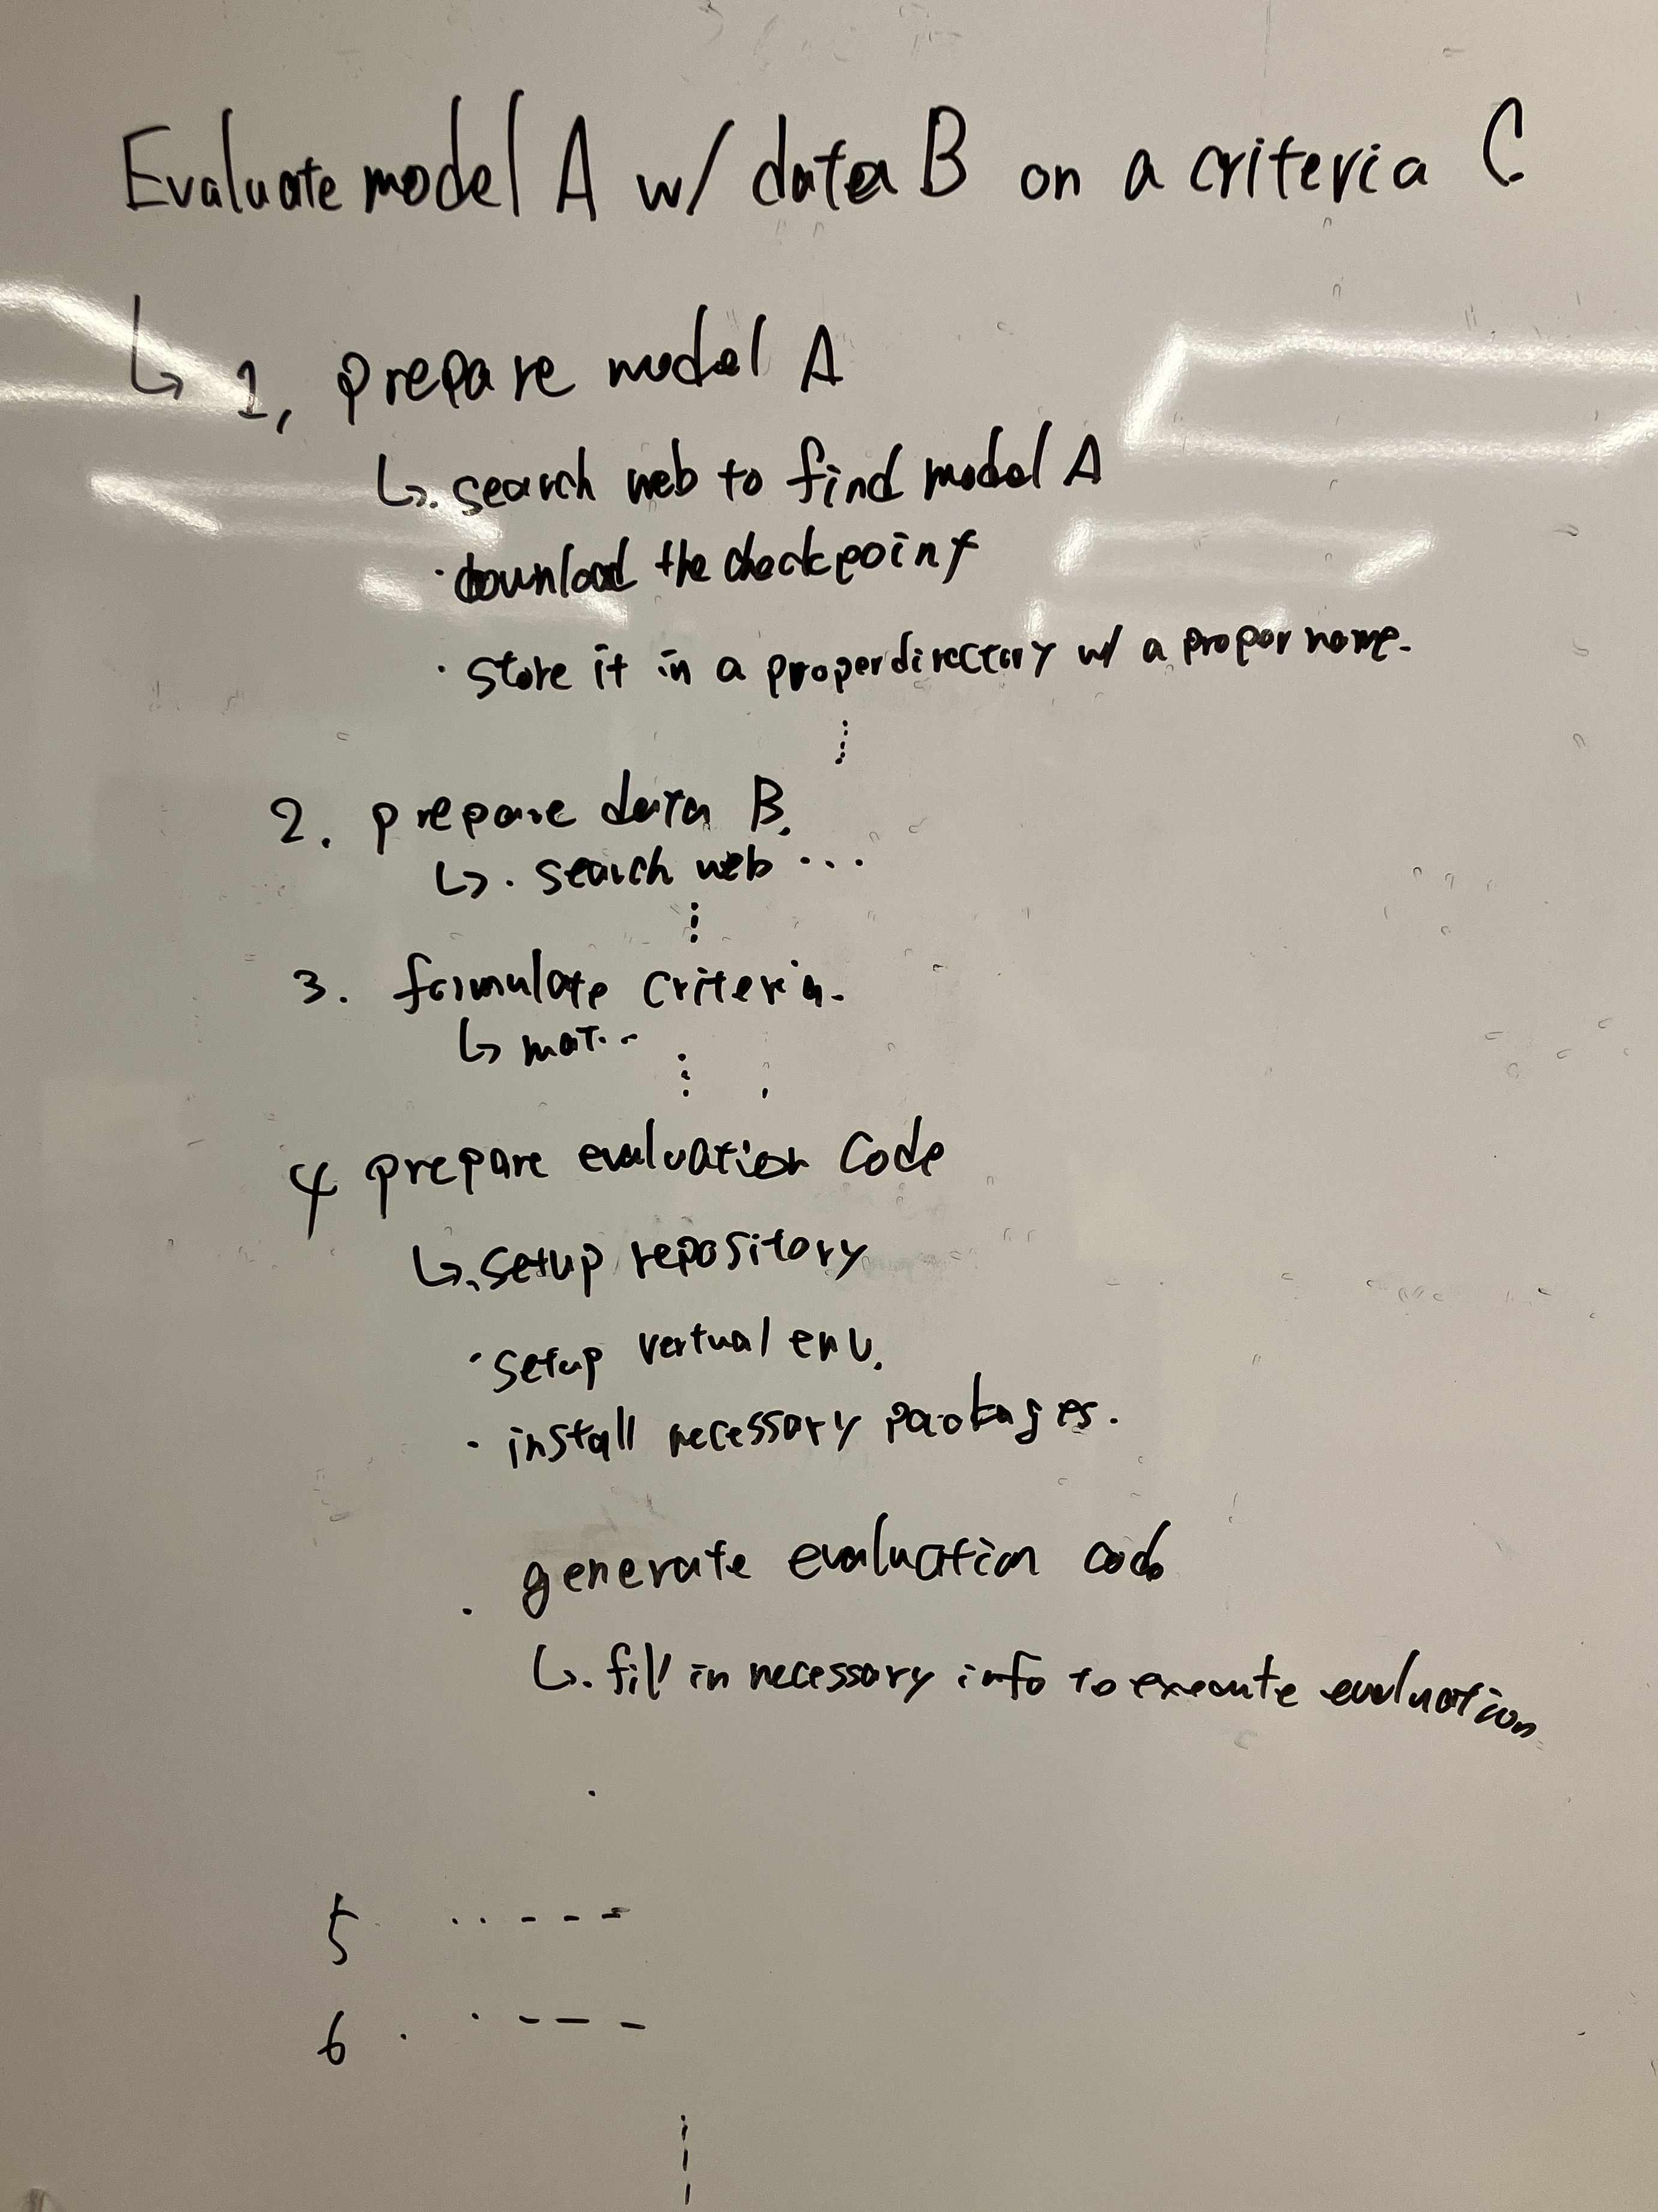
\includegraphics[width=0.5\textwidth]{figs/verification_instantiation.jpg}
%     \caption{Verification Instantiation}
%     \label{fig:verification_instantiation}
% \end{figure}

% As evident upon reading, this process is highly challenging to automate. Even research confined to the realm of computers, such as research of computer science, requires accomplishing a vast number of complex tasks. For research that necessitates physical realization in the real world, the development of robotics and embodied agents are necessary. Regarding the question of where and how to tackle these problems, I will provide my perspective in the later chapter. However, it is important to note that unless the research is constrained by questions and hypotheses, aiming for true automation will inevitably require overcoming these challenges

% To reiterate, this process can be accomplished through the automation of actions, and it does not necessarily require unique technological developments for research automation. For instance, in studies that are entirely computer-based, automating all actions within the computer system would suffice. In recent times, attempts have been made to have language models operate computers, and the progress in such research corresponds to the advancement of automation in this process. If the research involves activities in the physical world, achieving full automation of human movements (or their equivalents) would make this process feasible. Therefore, research focused on developing humanoid robots that can move like humans will contribute to the automation of this process.

% % Once a hypothesis has been established, a verification plan is created to determine how to verify it. The specific method of verification depends on the subject being investigated, making this aspect of research difficult to structurize and automate in a unified way.

% % However, in many empirical sciences, the likelihood of a hypothesis is evaluated based on statistical significance. This is done by \textit{hypothesis testing} in practice. As this is a hypothesis test, it can only reject the null hypothesis, rather than directly determining the correctness of the hypothesis. Therefore, it can only be said that the hypothesis has survived for the time being. The belief that the surviving hypothesis is more likely to be valid is the basis for decision-making.

% % In any case, humans seem to use statistics or probability as the basis for assessing the validity of a hypothesis. In other words, I seem to concede to consider a hypothesis as plausible if something that cannot happen by chance, such as observing the same number repeatedly. This is based on the assumption of the ``principle of confirmation,`` which assumes that if the number of observations increases, it can be considered more reliable, and the ``principle of uniformity,`` which assumes that things will continue to proceed as they have been if the conditions remain the saus. These beliefs ultimately serve as the basis for verification and scientific knowledge production. 

% % I will not delve into the validity of these beliefs here. What matters is that my research activity follow a practice that ``when a hypothesis is present, and a certain criterion and procedure are prepared, and the hypothesis is considered valid according to that procedure, I consider it valid.''

% % In theoretical research, sometimes there is no verification plan. Theory is a hypothesis, and its validity is determined separately through verification (not in the sense of whether it is mathematically valid, but for example whether it explains physical phenomena or not). However, in complex modern science, theorists propose a theory, and experimentalists verify it.

% % Therefore, it is understood that in current research practice, shared knowledge in the form of papers may not necessarily provide a complete answer to a given question. This is similar to research on negative data. Negative data cannot solve the unknown initially declared, but it can reduce a certain degree of uncertainty towards it. This is because the validity of the presented hypothesis may have decreased somewhat. If this is the case, each research shared in the form of a paper may be more appropriate to describe as "reducing uncertainty towards the unknown," rather than "making the unknown known." This can become complicated when scrutinized strictly, so let's put this aside for now and continue to discuss how "producing new knowledge" is research.

% % In reality, conducting research is expected to be done with limited resources (time, funding, computing resources, people, etc.). Therefore, it is necessary to consider these resources when determining the verification approach. After a research design is determined at an abstract level, the feasibility of the research plan is roughly evaluated through a simple problem setting. This is known as a pilot study.



% \subsubsection{Verification Execution}
% Finally, the instantiated research plan is executed according to the prescribed procedures. In verification design, I am crafting the essence of the verification, and during verification instantiation, I am preparing it to be executed in a concrete and feasible manner. Therefore, there are almost no tasks to be done in this process. The preparation for verification, being distinct from the actual execution of verification, is not a verification in itself. With this understanding, I have adopted this formal classification for the current context.
% \footnote{
% Typically,``experiments'' refers to the data generation process and subsequent analysis and interpretation are conducted separately. However, since I am discussing a verification plan in this context, all of them are in the same single plan. Therefore, please note that what emerges from executing the verification plan is not data but the verification results.

% In many empirical studies, the data generated from experiments is often used not only for the verification of hypotheses but also for generating new hypotheses or giving some insights. However, as hypothesis generation and hypothesis verification play different roles in knowledge production, I do not assume any uses of the generated data beyond verification in this context. Of course, please note that this does not imply that such actions are prohibited in practice. Data analysis will be discussed in a separate section.
% }

% \subsubsection{Starting from Verification Design}

% As mentioned above, I believe that the verification process can be divided into three stages: formulating a verification plan, preparing for the execution of the verification plan, and executing the verification plan. Among these stages, the execution of the verification plan and the preparation for it require interaction with the physical world in many fields. For example, in certain fields, you may need to purchase and raise rats for training, while in others, you may need to observe physical objects directly. On the other hand, formulating a verification plan is a process that is purely confined to the human mind in a wide range of fields. Therefore, it can be a good idea starting from automating verification design process.

% As mentioned earlier, in the case of empirical sciences, testing is often performed. Therefore, data is first generated, processed, and finally verified using the processed data. If I summarize the process of generating and processing raw data as data generation, this process can be broadly divided into data generation and judgment based on verification criteria. It may be rather said that the act of research itself is a process of repeatedly generating data and performing some kind of processing on it.

% I separated the verification plan from the verification because I want to separate the description and execution of the process. The verification plan is analogous to coding, while the verification is more similar to executing the code.

% The output of this process is usually wrtitten in the result section in the paper.

% \section{Conclusion}
% In this chapter, I discussed what research is. Research is the act of producing new knowledge for a community of constituents capable of forming shared beliefs. I characterized the production of new knowledge as the process of posing unanswered questions, generating hypotheses in response to those questions, and verifying them. Additionally, starting from the standpoint that knowledge is belief, I also presented the depiction of research as belief updating.
% \textcolor{red}{TODO}


% \chapter{Challenges and Ideas}
% In Chapter 2, we examined the definition of research and its implications, and in Chapter 3, we provided an overview of past efforts related to the automation of research. In this chapter, based on these, we will reorganize the challenges towards realizing an autonomous and general artificial intelligence capable of conducting research.

\subsubsection{Challenges}
In Chapter 2, we highlighted several challenges in realizing an AI capable of verification. First and foremost, the AI itself needs to understand what verification is, and by what criteria a sequence of actions qualifies as verification. Ideally, it would be preferable for the AI to contemplate and understand from scratch what verification is. However, many humans don't do this either, and as discussed in Chapter 2, the philosophical debate on precisely defining verification is still unresolved. Therefore, it's harsh to demand this of a machine. At the very least, the machine needs to thoroughly understand and proficiently use verification concepts that humans employ, such as statistical hypothesis testing, from first principles.


Second, the AI must be able to formulate detailed and complex plans to verify a hypothesis. With the advancements in language models in recent years, we are now much more capable of formulating superior plans than before. However, devising detailed plans remains a challenging issue.

Third, it has to be prepared to carry out these plans and execute the plan with the combination of human-like complex actions.As mentioned in Chapter 2, to achieve this, the AI must be able to search for, create, purchase, and manipulate equipment with almost the same degree of freedom as humans, requiring it to exhibit extremely sophisticated and complex behaviors. This is an immensely challenging issue, and it might even be fair to say it's one of the biggest bottlenecks in realizing an intelligence capable of generic and autonomous research. Laboratory automation have attempted to address this challenge in real world by developing robots. We will discuss the case within the computer below.

For AI to execute research on a computer, it must perform any operation within the computer. For instance, machine learning research entails, setting an environment, preparing datasets and models, and writing and executing codes. To allow AI to prepare these without human intervention, the AI itself must be able to autonomously search the web, select data, download it, and so on. Furthermore, once the AI generates code for verification, it must operate the shell to execute it.

There are ongoing initiatives to enable language models to operate browsers \cite{nakano2021webgpt,act1}. While full browser operations might seem ambitious, there are already endeavors to allow language models to conduct searches \cite{mialon2023augmented}. If we achieve browser automation, it will greatly advance research automation involving web operations. Moreover, efforts like the open interpreter \cite{openinterpreter} aim to automate any computer action. This direction holds promise for automating all research confined within a computer. Although these studies are gaining traction in the machine learning domain, they're not always linked to research automation. We advocate recognizing this as a pivotal challenge in the realm of research automation.

In the field of machine learning, it seems that the discussion on automated validation has not garnered much attention until now. However, recently, the need for verification is recognized in the machine learning community beyond outside of the context of research automation. Studies like \textit{scientific claim verification}, which received much attention during the COVID-20 pandemic \cite{wadden2020fact}, or attempts to minimize hallucination \cite{dhuliawala2023chain} are examples of them. These are not attempts to automate validation in research. Therefore, these findings cannot be directly applied to the automation of research validation. However, we expect that these studies will provide useful insights for the future development of artificial intelligence capable of understanding validation.

\subsection{Combining Questions, Hypotheses, and Verification}

一度終わった研究を後から振り返った時にこの構成になっていることに言及する。やっている途中は必ずしもそんなに綺麗に進まない。

研究の構成要素である問いの構築、仮説の生成、仮説の検証について説明しました。実際の研究は極めて複雑な試行錯誤的なプロセスであり、これらが最初に想定していた通りそれぞれ一回ずつしか行われないということは稀です。研究ができる AI を作るためには、そのような複雑な研究実践が可能でなければならないように思われます。そこで、本セクションでは、そのような AI を作るために考慮すべきであろう事項について検討していきます。また、問いの構築、仮説の生成、仮説の検証のいずれの自動化においても共通する課題についても議論します。

Night Science

- 仮説駆動型研究が新しい発見を妨げる可能性がある 
\cite{yanai2020hypothesis}

\subsubsection{Human Research Practice and Knowledge Production System}
In actual research, while addressing the initial question posed, another question may arise and the focus may shift to that new question. Also, before reaching the final hypothesis that gets reported, several different hypotheses are tested repeatedly. Like this, the actual practice of research is complex.\footnote{
For example, the concept of \textit{night science} as proposed by Yanai and Lercher symbolizes the such complex reality of research practice \cite{yanai2019night}.
} When compared to this trial-and-error process, the framework I have proposed may seem overly simplified at first glance. However, I believe that the framework I proposed encompasses these human practices as well.

The framework I presented claims that in the process of generating knowledge, there is always a construction of questions about the process, the generation of hypotheses, and the verification of these hypotheses. I have not specified how these are done. Therefore, a question might have arisen while working on a different question, or it might have been directly derived to achieve a specific goal. Similarly, a hypothesis might have been developed after multiple comparisons with real data, or it could be something that came to mind while walking. What I'm arguing is that, regardless of the diverse methods employed, when an activity is termed research, there should always be a stage where questions related to the knowledge produced, the generation of hypotheses, and the verification of these hypotheses are addressed. This may indeed look like a linear process when abstracted, but given that it allows for trial-and-errors as its internal implementation, I believe it encapsulates the complex practices of human research.

Furthermore, setting aside whether a strict methodology like that of research is required, I believe that all endeavors to transform the unknown into the known, to some extent, inevitably involve the construction of questions, the generation of hypotheses, and the verification of these hypotheses. In other words, I think this framework might be an embodiment of the very act of turning the unknown into the known. In this sense, this framework might be better understood as a fundamental unit in research.

\subsubsection{Countless Question, Hypothesis, and Verification in Research Process}
We generate countless questions and hypotheses, including implicit ones, for the purpose of creating a single question or hypothesis, or for planning and preparing for single verification.

For example, when questioning how an unresolved issue can be solved, we might ask why this problem hasn't been solved so far, or if there are any studies of similar challenges being addressed. In response, we might consult literature or recall our own memory, hypothesizing that ``This could be the reason it hasn't been solved,'' or that ``This could be useful in solving the current challenge.'' We repeat this process innumerably to eventually construct an answer to the original question. Similarly, when planning verification, we implicitly pose many questions and formulate numerous auxiliary hypotheses.

To generate a plausible hypothesis, there must be sufficient grounds to believe it is valid. These grounds could be knowledge from our own memory, descriptions from newly researched literature, opinions from other researchers, or some belief, such as natural law should be simple. In addition, to examine the validity of the hypothesis, we might try simple tests. For example, we might create a toy model to represent the hypothesis and examine its behavior, or conduct preliminary experiments. In other words, each time a plausible hypothesis is generated, it undergoes a sort of verification, whether implicit or explicit, and to varying degrees of simplicity.

In this way, to conduct research, we pose countless questions and hypotheses and conduct several simple  experiments to verify the plausibility of the hypothesis if necessary. This is because research is an endeavor facing the unknown, and this process contains a lot of uncertainties. By gradually reducing these uncertainties through trial and error, research progresses. This gradual reduction of uncertainty seems essential, especially when tackling difficult questions that no one in the world knows the answers to. Therefore, AI capable of conducting research should autonomously be able to generate numerous questions and hypotheses as needed and choose more plausible hypotheses through simple verification during the knowledge production process.

% 私たちは、一つの問いや仮説を生成するために、あるいは検証の計画や準備をするために、暗黙的なものも含めると無数の問いや仮説を生成しています。

% 例えば、ある解決されてない課題をどのように解くことができるか問うた場合、ではそもそもなぜこの問題はこれまで解かれてこなかったのだろうか、似たような課題に取り組んでいる事例はないだろうか、と問うかもしれません。これに対して文献を調べたり過去の知見を思い出したりして、これが原因で解けなかったのではないか、これは今回の課題の解決に使えるのではないか、といった仮説を立てるでしょう。これを無数に繰り返して、最終的に元々答えたかった問いに対する答えを構成します。また、検証の計画を立てる際にも、私たちは暗黙的に多くの問いを立てて無数の補助仮説を立てています。

% 確からしい仮説を生成するためには、その仮説が妥当であると信ずるだけの根拠がなければなりません。その根拠となるのはは自分の記憶にある知識かもしれませんし、新しく調べた文献の記述かもしれませんし、他の研究者の意見かもしれません。これに加えて、確からしい検証をするために、私たちは試してみる、すなわち簡単な検証をすることもあります。例えば、仮説を表現するトイモデルを作って挙動を調べてみるかもしれませんし、プレ実験をしてみるかもしれません。

% このように、私たちは一つの問いを作り、それに答える一つの仮説を作り、それを一度検証するために、無数の問いと仮説を立て、必要とあれば仮説の確からしさを簡単に検証するいくつもの実験を行います。これは、研究が未知に立ち向かう営みであり、その過程にはいくつもの不確定な要素が存在するからです。それらの不確実性を一歩一歩試行錯誤的に削減していくことで、一つの研究が進んでいくように思われます。このような漸進的な不確実性の削減は、特に誰も答えを知らないような難しい問いに挑戦する際には不可欠であるように思われます。従って、研究ができる AI もこのように、必要に際して問いや仮説を生成し、簡易的な検証によってより確からしい仮説を選択するということを自律的に行えるようになる必要があるでしょう。


\subsubsection{Discovering New Questions}
Researchers often set out to solve one question, only to find themselves discovering an entirely unrelated question in the process. This new question, unrelated to the original question and even its underlying purpose, may lead them to pivot their research focus and potentially make significant scientific discoveries. Since research is full of uncertainty, it's not uncommon to be unable to foresee everything from the start. Thus, this discovery and shift of question is not rare.

If an AI capable of conducting research were tasked with achieving a single objective, such serendipitous discoveries might not occur. This is because any new questions it finds, no matter how intriguing or scientifically important, may not be directly relevant to achieving its predefined goal. Therefore, to encourage an AI to uncover such unrelated questions, it might be necessary to set multiple objectives or a broader high-level goal that encompasses both sets of questions, like ``understanding nature.'' Additionally, to switch from the current question to a new one, the AI would need to evaluate which of the two questions holds more value.

% 研究者は、ある問いを解くために別の問いを立てるだけではなく、その問いに答えようとする中で、最初の問いやその背後の目的とは全く関係ない別の問いを見つけることがあります。そして研究の途中でそちらの問いに取り組むことに切り替え、その結果大きな科学的発見を成し遂げることもあります。不確実性が高い研究という取り組みにおいては、最初から全てを見通せることは多くありません。したがって、このようなことが起こることは少なくありません。

% もし 研究ができる AI にある一つの目的を達成することを目指させるとしたら、このようなことは起き得ないでしょう。なぜなら、そこで見つかった問いはどれだけ面白くてもどれだけ科学的に重要でも、その目的を達成するために必ずしも重要とは限らないからです。したがって、AI にこのような問いの発見をさせるためには、複数の目標を持たせる、あるいは両方の問いを包括するようなより大きな(例えば「自然を理解する」のような)大きな目標を持たせる必要があるように思われます。加えて、現在やっている問いに取り組むのをやめて新しい問いに取り組む意思決定をするためには、AI はこれらの異なる二つの問いのどちらが価値があるかを比較しなければならないように思われます。

\subsubsection{Feedback from Verification Result}
化学自動化論文の内容もここに追加する

In research, it's not always common for the initial hypothesis to directly answer the question posed. Rather, the process typically involves revising the hypothesis based on the results of verification, followed by additional rounds of testing. This cycle of hypothesis revision and retesting is crucial in the journey toward finding answers to the posed questions, especially when seeking unknown answers, as mentioned earlier. Consequently, it seems necessary for an AI capable of conducting research to have the ability to revise its hypotheses based on the outcomes of these verifications.
% 研究では最初に建てた仮説がそのまま問いの答えであるという場合は必ずしも多くはありません。検証の結果を踏まえて、仮説を修正し、再度新たな検証をし、というサイクルを繰り返すことで、問いの答えへと近づいていきます。前述したように、これは未知の答えを発見しようとする以上必要となってくる過程です。したがって、研究ができる AI もこのような検証結果を踏まえて仮説を修正できることが求められるように思われます。

However, when the result for verification were negative, identifying the cause of the result is not as straightforward as one might think. This is because the verification relies on numerous implicit and explicit hypotheses and all of them can be the cause of the result \cite{sep-scientific-underdetermination}. The cause may be the proposed main hypothesis, a premise behind the hypothesis, an auxiliary hypothesis, an observation, an experimental instrument, or all of them. An AI that can conduct research must identify which of these possibilities is the cause. Once the candidates for the cause are determined, the AI has to generate a more plausible hypothesis based on the results of verification, as we have discussed so far.

In science, to identify the cause, it would be necessary to appropriately interpret the data generated by experiments. However, what one reads from the data can change depending on the individual's beliefs, prior knowledge, and what they expect to find. Therefore, these verification results may be reinterpreted multiple times, and with each reinterpretation, the hypothesis that needs to be revised may change. Ideally, AI capable of conducting research should be able to interpret verification results with these possibilities in mind.
% 科学であれば、原因を特定するためには、実験によって生成されたデータを適切に解釈する必要があるでしょう。しかし、データから何を読み取るかは、その人の持つ信念や事前知識やそこから何を期待するかによって変わり得ます。したがって、この検証結果は何度も再解釈される可能性があり、その度に修正すべきだと思われる仮説が違ってくるかもしれません。研究ができる AI は理想的にはこのような可能性も視野に入れて検証結果を解釈していくことができるようになることが望まれるでしょう。


\subsection{Common Challenges}

\subsubsection{Open-Endedness}
One of the major challenges that can be a common issue for any process, as pointed out in prior research as well  \cite{coley2020autonomousII}, is how to execute these tasks in open-ended situations. For instance, in the automation of experiments, robots use experimental equipment selected, prepared, and set up by humans. However, humans do these tasks from scratch with their own hands. Humans do not use a given corpus of papers; instead, they search for and use them on their own. Candidates for hypotheses are not explicitly provided; humans begin by identifying potential hypotheses. Even when formulating questions that serve a particular goal, humans set that goal themselves. 

In many cases in research automation, these elements are pre-determined by humans. How to let machines autonomously perform these tasks starting only with the same initial information given to humans is crucial in realizing an autonomous artificial researcher. Moreover, having this kind of freedom is essential to achieving a general artificial researcher as well. This is because if we impose constraints on AI to research only within specific research questions or hypothesis spaces defined by humans, it cannot become an AI capable of conducting arbitrary research. Therefore, a significant challenge is how to make AI acquire complex foundational skills and fundamental reasoning abilities to realize these capacities.

\subsubsection{Generality}
汎用性がなぜいるかなどの説明?上の定義はそもそもそういうモチベーションから始まってるので、ここでわざわざ書かなくても良い。

特定の研究課題に特化すれば、問いの構築、仮説の生成、仮説の検証を実行できるような機械はすでに開発されています。これまでのセクションでこれらの概念の定義を改めて検討したのは、研究ができる AI とは特定の研究課題に特化した方法でこれらを実行するのではなく、どのような研究対象に対してもこれらを自律的に遂行できる AI であることが望まれるからです。このような汎用的な研究ができる AI をどのように実現するかというのが課題です?

\subsubsection{Autonomy}
As mentioned in the previous section, there are several attempts to automate the entire research process. A seminal early works are Adam \cite{king2004functional}, and Eve \cite{williams2015cheaper}. These are closed-loop scientific discovery systems that autonomously execute everything from hypothesis generation to research planning, based on logic AI and robotics. Furthermore, there is closed-loop automation in some research on automation using scientific workflows \cite{gil2017towards}. These are highly autonomous research automation. Recently, there has also been a movement to create autonomous agents based on language models to tackle scientific problems \cite{wang2023survey}.

However, most of studies on research automation have targeted  only specific tasks within a sub-process of the entire research process. For example, symbolic regression focuses on automating hypothesis generation, while experiment automation pertains to data generation for hypothesis creation and testing.

Furthermore, even in the case of closed-loop research automation,  full automation of all processes of science is yet to be realized \cite{zenil2023,coley2020autonomous,coley2020autonomousII}. One of the biggest issues is that the objectives, problems, and questions of research are given by humans \cite{coley2020autonomousII}. We discussed in Chapter 3 that there are not many studies that have attempted to automate the construction of questions. And while we pointed out in Chapter 2 that automating the construction of questions can lead to an infinite regress from the perspective of autonomy, specifying the high-level goals underlying the questions remains a significant challenge \cite{coley2020autonomousII}. Also, even after the construction of the question, there is the issue that humans are providing machines with a search space that is far more restricted than what humans themselves are given. For example, generating hypotheses from an open-ended hypothesis space has not yet been realized \cite{zenil2023,coley2020autonomousII}, and to put it in extreme terms, while humans might prepare experimental equipment from scratch, machines are given those as a given. 

% To begin with, the realization of a fully autonomous artificial intelligence is still one of the major goals yet to be achieved, not just in research. Therefore, a lot more foundational research will likely be needed to accomplish this.

% Many automation studies primarily target specific tasks within a research process. For example, symbolic regression focuses on automating hypothesis generation, while experiment automation pertains to data generation for hypothesis creation and testing. However, as mentioned earlier, some studies, such as automated research workflows and self-driving labs, aim to automate the entire research process. 

% Coley et al. discuss the advancements in automating scientific discoveries in chemistry \cite{coley2020autonomous}. Their discussion is not limited to automating chemistry but extends to the broader context of automation of science. The paper delves into the insightful topics of automated discovery, including defining scientific discoveries and criteria for assessing their autonomy. In the subsequent paper, Coley et al. organized the existing automation studies based on which processes of scientific workflow are automated \cite{coley2020autonomousII}. In that paper, they point out several challenges for science automation, ranging from dataset handling to physical and computational autonomous validation. 

% Autonomous agent for scientific problem \cite{wang2023survey}

% , and in recent years, there are attempts to automate the entire process using language models.

\subsubsection{Generality}
As we have introduced so far, there are several attempts to automate research through versatile approaches. For example, the automatic generation and discovery of hypotheses \cite{kang2022augmenting,chan2018solvent,wang2023learning,xu2023exploring} or questions \cite{lahat2023evaluating,liu2023creative,oppenlaender2023mapping,surita2020can} from research papers is an approach that can automate research across a wide range of academic fields, from the humanities to natural sciences. Additionally, efforts to create general-purpose robots  \cite{yachie2017robotic}, foundation or generalist models \cite{singhal2023towards,taylor2022galactica}, or to incorporate the inductive bias for understanding physics can be considered initiatives towards general-purpose system.

However, most automation studies target specific challenges in particular research fields. It seems that the goal of creating an AI capable of conducting any research is not receiving much attention. As explained in Chapter 2, in order to create such intelligence, it would be necessary to understand the high level concept of research, question construction, hypothesis formulation, and hypothesis verification, and to be able to execute them appropriately depending on the subject at hand.



% どのような研究対象に対しても問いを立て、仮説を生成し、仮説を検証できるような人工知能を作るためには、これらを汎用的な方法で実行する必要があります。このように

% \subsection{Challenges}

 % \subsection{General and Autonomous Question Construction, Hypothesis Generation, and Hypothesis Verification}

 % In Chapter 2, we explained that in order to create an AI capable of conducting any research, it is deemed necessary to realize the formulation of questions, generation of hypotheses, and validation of these hypotheses as a combination of universal skills applicable to all research. In this section, we will revisit and organize the potential challenges in achieving an AI that can conduct each of these processes.


% \subsubsection{The Difficulty of General Hypothesis Verification}
% I recognize that the the way to verify a hypothesis is strikingly diverse, as it can significantly differ depending on the subject of research. For instance, if one wishes to study the behavior of rat, they may need to train the rat. On the other hand, if you want to test a theory of particle physics, you may have to construct and run a huge particle accelerator. In the field of history, the existence of historical records might serve as evidence, while in mathematics, the verification process revolves around the proofs themselves. Due to this high degree of flexibility, hypothesis verification can be the most challenging aspect to automate for realizing a ``general'' artificial researcher.

% \subsubsection{Feedback from Verification}
% In the first place, the act of verification is a highly challenging process. Firstly, as mentioned earlier, inductive approaches cannot verify hypotheses in the same way as deductive reasoning. Also, I notice that hypothetico-deductive method, which involves verifying claims derived from a hypothesis to confirm its validity, is still widely used today. However, verifying a deduced claim does not support the hypothesis because there may be many hypothesis that can result in the same deduced claim. In response to these, Karl Popper proposed that while hypotheses cannot be confirmed, they can be falsified \cite{sep-scientific-method}. However, in practice, the verification of hypotheses involves implicitly relying on numerous auxiliary hypotheses. When using experimental apparatus, it requires many assumptions to trust them. Even when an experiment fails, determining whether the hypothesis was incorrect or the experiment itself was flawed is not as straightforward as one might think. Thus, there is inherent uncertainty in attributing the results of verification to a specific cause \cite{chalmers2013thing,sep-physics-experiment,sep-scientific-underdetermination} as I have discussed in the section of hypothesis generation. Furthermore, all reasoning and observational evidence are inevitably influenced by some form of theories, individuals, or societal factors \cite{sep-science-theory-observation}. Therefore, it is necessary to carefully examine them to ensure that they are not distorted by unintended influences.


% \subsubsection{Question Construction}



% Realizing AI that construct a ``good'' question in a generic way is challenging. As discussed in Section \ref{section:the-relativity-of-knowledge-production-to-society}, research is relative to society and different criteria can be considered for what makes a ``good'' question. Thus, some human perspective on the ``goodness'' of a question must be incorporated. We need to discuss what we consider good, what we should prioritize, and how to incorporate the value to AI.

% \textcolor{red}{TODO}

% Moreover, determining inputs to the question construction module is not trivial. In hypothesis generation, the question is the primary input, whereas in verification, it's the hypothesis. However, question formation take any input. Once you seriously try to identify the origin of question, you will encounter infinite regress. This is a unique problem that arises when aiming for a general-purpose and autonomous artificial researcher. This is because the issue revolves around how much input can be assumed while still being considered autonomous, given that it can potentially take any input.

% \cite{wang2023skillqg}

% neural question generation \cite{pan2019recent}


% \subsubsection{Hypothesis Generation}



% \subsubsection{Hypothesis Verification}



% Creating AI that autonomously verifies hypotheses is challenging. While current models can mimic human verification, truly understanding the verification strategy demands more work. Sometimes, they even need to devise the verification measure themselves.

% The biggest challenge for autonomous verification is the need to freely move around in the real world or within a computer, and to manipulate objects within that world at will. We believe this to be one of the greatest barriers to full research automation. Laboratory automation have attempted to address this challenge in real world by developing robots. We will discuss the case within the computer in Section \ref{section:behaviour-inside-the-computer}.

% \subsubsection{AI Capable of Peer Review}

% Given the difficulty of these challenges, automating peer review could be a strategic starting point. This is because peer review is a universal process across diverse research fields and it assesses the validity and quality of problems, hypotheses, and verification methods, which is easier than generating them. Despite some progress, full automation is still elusive \cite{yuan2022can,schulz2022future}.


% \subsection{Behaviour inside the Computer}
% \label{section:behaviour-inside-the-computer}


% Lab Notebook?
% \subsection{Dataset of Research Process}
% It is important to establish the necessary infrastructure for research automation. The two pillars of research automation are the development of basic models that incorporate academic knowledge and the construction of data sets. The development of an infrastructure model that incorporates scientific knowledge has already been proposed in many places and is actually under development, so I will not emphasize its necessity here again. Also, regarding data sets, the construction of data sets for the acquisition of scientific knowledge has been done in various places as well, so I will not emphasize that here either.

% Instead, we propose here to construct a research process dataset. A research process dataset is behavioral log data that incorporates all possible tasks throughout the entire process of the study, from start to finish. Ideally, individual tasks should be labeled as to whether they correspond to question construction, hypothesis generation, or hypothesis testing. We believe that building such a data set is important because, as explained in the Literacy section of Chapter 2, the current paper is not a data log of the entire research process. This makes it difficult to be data-driven and end-to-end learning how to do research itself. I believe that building a research process will help solve these problems and increase the likelihood of more flexible intelligent agents.

% However, building a dataset of the research process seems daunting. This is because researchers who do not currently keep research logs would have to go to the trouble of recording their research process.\footnote{
% In an experimental laboratory in the natural sciences, it is common to take research notes, so it may not be that difficult to record more detailed processes as an extension of this practice. However, in the machine learning field, the culture of taking research notes does not seem to be that common. (We think it is common to keep logs of experiments, but it seems to be rare to describe the details, for example, where and how the data was obtained.) 
% } Therefore, it seems necessary to devise a way to make it easier for researchers to keep logs. It may be to manage the research process on GitHub, or to take research notes as in natural science research, but it is important to discuss how to achieve these things.

% Being able to construct a dataset of the research process would be ideal, but may not be immediately feasible. As an alternative, it seems important to create a dataset designed to automate question construction, hypothesis generation, and hypothesis testing. At its simplest, one might start by building a dataset of papers labeled with the parts that correspond to the question, hypothesis, and test, respectively. This would be a relatively simple but important step in achieving a generic artificial researcher.

% Alternatively, instruction tuning could be done by viewing question construction, hypothesis generation, and hypothesis testing as tasks, respectively. This would produce a language model that can execute question construction, hypothesis generation, and hypothesis testing with greater fidelity. This could be the foundation for a general-purpose, autonomous artificial researcher.





% In the medium to long term, it's essential to devise ways to ensure that AI doesn't engage in research that could be dangerous to humans. 

% In the long term, we must contemplate how to construct a knowledge system that are mutually translatable between human society and AI society. While these issues may not arise in the short term, it's crucial to engage in discussions now, looking towards the long-term future.

% \subsubsection{Understanding}

% Extensive discourse transpires concerning scientific discoveries. Yet, discussions pertaining to scientific comprehension remain relatively unexplored. Krenn et al. delve into the conundrum of what it entails for a machine learning agent to not only unearth scientific knowledge but also to comprehend it \cite{krenn2022scientific}. They adopt a human-centric stance, positing that an agent's ability to offer explanations comprehensible to human scientists signifies the existence of its scientific understanding.

% sun-rise \cite{leslie2023does}

\section{Ideas for Elucidating Challenges}

言語モデルすごいし、言語モデルでやってくの考えたいよね。汎用的なのを言語モデルでやってみるならどんなになるだろう?→できるだけ汎用的な指示ということになるよね!みたいな

\subsection{Prototyping General and Autonomous Artificial Researcher}

Realizing a general and autonomous AI capable of research is an exceptionally challenging issue that will likely take a long time. The challenges mentioned in the previous section are just the tip of the iceberg, and there are undoubtedly many more yet to be identified. Therefore, it seems crucial to start by identifying and addressing unknown challenges to reduce uncertainties. A good starting point might be to develop a prototype of a general and autonomous AI capable of research.

Let's discuss what this prototype might entail. As reiterated earlier, research, we believe, consists of constructing questions, generating hypotheses, and verifying these hypotheses. Thus, it seems appropriate for this prototype to consist of three main modules: question construction, hypothesis generation, and hypothesis verification. The question construction module takes any input and produces a question. The hypothesis generation module takes this question as input and produces a hypothesis. The hypothesis verification module takes the hypothesis as input and provides verification results.

For the prototype to be autonomous, human design, implementation, and intervention should be minimized. Consequently, each module, aside from receiving minimal inputs, should autonomously gather information from the world humans typically interact with. For instance, aside from the question input from the question construction module, the hypothesis generation module shouldn't have predetermined inputs. This module could have touchpoints with the physical world or the digital realm, acquiring necessary information and generating hypotheses as humans do.

Furthermore, for the system to be general, the internal workings of each module mustn't depend too much on specific research topics. For example, if the verification method is an algorithm planning and executing experiments for a specific physics research, it can't be used for psychological research. Also, if the verification method is an algorithm to plan and conduct experiments, it can't be used for deductive research. The inner workings of the hypothesis verification module should be as minimal as possible, limited to only what is necessary for hypothesis verification. 

This is akin to an abstract class of research. Creating a system that meets both autonomy and generality requirements while properly constructing questions, generating hypotheses, and verifying them only with this abstract system is too challenging, even in simpler scenarios. Hence, it might be necessary to impose some constraints on this abstract framework initially. Discussing the extent of these constraints, why they're needed, and how they can be eliminated will help elucidate the challenges in realizing a general and  autonomous AI researcher. By identifying these challenges and turning them into research themes, and then advancing foundational research, we believe we can more efficiently approach the goal. In the following, we will list up such potential constraints to provide a first step.

\subsubsection{Candidate Constraints in Prototyping}

% \subsubsection{Grand Goal is Given}
As we've emphasized repeatedly, constructing questions from open-ended situations is a challenging task where even a starting point for resolution is not visible. Therefore, it seems prudent to start by determining in advance what the input for constructing the question should be, separate from the unrestricted information sources that the module can access. For such input, it might be appropriate to consider the overarching goal we ultimately want to achieve as the minimal input. As stated in Chapter 2, not all research questions are necessarily constructed to achieve some grand goal. However, many studies build their questions by breaking down such objectives. Consequently, if research can be conducted to construct questions from overarching goals, then a vast majority of human-conducted research, and notably ``meaningful'' research, potentially becomes feasible.

% \subsubsection{Research is Completed Entirely within a Computer}
One of the biggest bottlenecks in realizing a fully general and autonomous artificial researcher is the necessity for complex actions in the preparation and execution of verification. Especially, developing a robot capable of acting freely in the physical world like humans is an extremely challenging task, and it carried difficulties beyond just AI research. Therefore, it seems reasonable to first consider research that is confined within a computer for prototyping purposes. Specifically, it means envisioning a world where AI can interact not in the physical realm but within the computer environment. Some computer science research falls under this category. Of course, realizing an AI that can freely operate within a computer is also a very challenging issue, but it seems more feasible than an agent freely operating in the physical world. The purpose of prototyping is to materialize the concept, even if it's rudimentary, and identify challenges. Therefore, it seems desirable for prototyping to first limit the target environment to within a computer and wait for the advancement of foundational research for the realization of free activity in the physical world.

% \subsubsection{Verification is Limited to Humans'}
The issue that allowing machines to conduct research entirely autonomously could result in constructing knowledge systems meaningless to humans arises when we try to let AI construct even verification from scratch. This is necessary if we want to truly say an AI can verify on its own. On the other hand, many people probably have no interest in generating knowledge that is meaningless to humanity. In the first place, even if such a thing were realized, humans might not be able to evaluate whether the AI has truly constructed a meaningful knowledge system for them. Also, I don't think human researchers always understand or construct verification from first principles. Therefore, it might seem harsh to demand these of AI. So, it seems preferable to first ensure that AI understands and can always use the verification methods that humans use. Specifically, we aim to make sure AI can always proficiently use experiments, statistical hypothesis testing, proofs, etc. By doing so, I believe there's a possibility to realize an AI that conducts highly generalized, autonomous research that is meaningful to humans.

\subsubsection{AI that Conducts Machine Learning Research}
Providing a grand goal or limiting the action space can restrict the targeted research field. We believe it might be beneficial to aim for the realization of AI that can conduct machine learning research as prototyping. Firstly, some machine learning research can be fully completed on a computer, meeting the aforementioned constraints. Furthermore, machine learning technology is essential for the realization of research-capable AI and currently serves as a foundational technology in many research fields. Thus, if machine learning research can be fully automated, it will not only advance the study of automating other research areas but also accelerate the automation across many disciplines. This suggests that starting with the automation of machine learning research might be a good approach to speed up the development of research-capable AI. Moreover, in machine learning, there are already efforts underway, such as AutoML and MLOps, to automate parts of the machine learning research workflow. These achievements will likely further assist in creating AI that can conduct machine learning research.

\subsubsection{Implementing Each Module with Large Language Models}

Considering the remarkable performance of recent language models and the necessity for general-purpose research, it seems reasonable to first represent each module as a large-scale language model. While there are increasing efforts to construct pipelines by connecting large-scale language models, we will prototype the overall research execution system by connecting language models in a similar manner. To ensure this system is open-ended and general-purpose, prompts given to these language models will consist only of general instructions that can be applied to many types of research. For instance, an instruction like "generate a hypothesis for the following question" is a command that can be given to a hypothesis-generating module in not just machine learning research but any field of research. Naturally, merely providing such instructions won't yield perfect results from the get-go, so there may initially be a need to provide additional auxiliary directions. However, even these instructions will be kept as general as possible.

For open-ended operations within a computer space, ideally, the system should only be given access to nearly all operations on the computer, akin to what an open interpreter does. Minimal access to web browsers, search engines, or shells might be acceptable, but provision of custom corpora or predefined hypothesis spaces should be avoided. If research can be autonomously conducted under such conditions, it would indeed signify that the system is capable of independent research.

I worked with a research group attempting to automate research, and together, we created a simple mock-up expressing such a concept \textcolor{red}{CITATION}. We assumed a given question and examined how much GPT-4 could generate and validate hypotheses using only the most general prompts possible. While this initiative is still in its early stages and is limited to very basic problem settings, based on our findings here, I hope to eventually develop a system that more closely resembles human research capabilities.

% We believe that automating machine learning research may be suitable to start with in terms of these decision axes. First, let's discuss bootstrapping. Many of the challenges to automating research will be how to get machines to acquire from experience what they are currently hardcoding and doing in the real world. Learning from experience is exactly what machine learning does, and in this sense, many of the challenges in realizing autonomous artificial researchers can be formulated as machine learning research challenges.

% Next, let us discuss feasibility. In the first place, many machine learning studies are conducted entirely on computers. As mentioned earlier, the greatest difficulty in achieving general automation lies in the interaction with the real world. Technologies related to real-world interaction are used for hypothesis verification rather than the verification itself. This requires advancements in robotics research. Therefore, to pursue the automation of the entire research process, it may be best to set aside fields that require interaction with the real world and initially focus on automating research that can be done solely on PCs. 

% Also, many attempts to automate machine learning processes have already been made. For example, in MLOps, various pipelines for automating tasks such as experiment management and training in machine learning have been proposed and put into practical use. AutoML, which is a field of machine learning research, has also produced numerous innovations in automating many of the tasks involved in machine learning. Moreover, the culture of machine learning and related engineering fields already has a wealth of knowledge and insights regarding automation. This means that we do not have to devote many resources to automating research domain-specific tasks. This allows us to focus on more essential questions in our quest to become general-purpose artificial researchers, such as ``How do we allow people to test hypotheses?'' Furthermore, many studies in machine learning and related research areas are open-source. Consequently, it is considered easier to retrieve information from papers compared to other fields. 

% Finally, we would like to discuss the impact on other sectors. As you are already aware, many research fields are currently using machine learning technologies. The AI for Science initiative, which aims to automate the scientific field, also uses machine learning technology. Therefore, the automation of machine learning research and better knowledge production will accelerate all of these efforts. For these reasons, we believe it is a good approach to start by automating a specific research project in the machine learning domain.

% \subsubsection{What Type of Research in Machine Learning Should We Start with and How?}
% There are many different types of machine learning research, but where should we start with automation? Even though we aim to automate the construction of questions, what types of research should we guide them to do?

% It seems that a example of the research appropriate as one a starting point is that on the zero-shot prompt proposal. First, the hypothesis (or proposal) in this study is the specific text of the prompt. This is much less expensive to implement, whereas many empirical machine learning proposals require composing an algorithm or architecture. Validation requires the automation of the task of preparing existing data and models, and this is certainly a difficult task. However, this is an extremely common task in machine learning research and is not unique to this research project. The ability to automate this task would benefit a significant amount of machine learning research. The validation criterion is also generic, as it is a typical validation criterion that compares the proposed group with the control group. We think we will first build a prototype by adjusting the LLM prompts, and the fact that there is no strict mathematical or logical manipulation, which language models are not good at, is another aspect that makes this research easy to do.

% With this in mind, one research project in which the author of this paper is participating is in the process of building a prototype of the pipeline of research for the prompt proposal \footnote{
% Link to the pipeline: \href{https://github.com/t46/mock-pipeline}{https://github.com/t46/mock-pipeline}
% }. It is currently still in the pilot stage and some parts are hard-coded, but will be updated as needed.

% What we have described here is just one example and a suggestion. We hope that more similar initiatives will emerge in other studies.


% We propose to start by building a research pipeline, connecting the modules of the knowledge production system. The research pipeline is a software system that takes input and generates knowledge as output, encompassing the sequence of processes involved in research. Since this process does not require human intervention, it can be considered as an autonomous research system. We propose this system to be composed of the sub-processes of ``question construction,'' ``hypothesis generation,'' and ``hypothesis verification.'' This creates a general system that is potentially applicable to any research. These sub-processes can be likened to abstract classes in programming. Each process automatically formulates appropriate questions, generates hypotheses, and performs verification based on the input. 

% Initially, we will assume a specific research problem, and this research problem can be a simple one. And the inner workings of detailed hypothesis testing and hypothesis generation can be guided (but not hard-coded) to achieve the desired results. Anyway, the high-level concept is to create the minimum necessary to automatically execute each process of question construction, hypothesis generation, and hypothesis testing. Then, by gradually making the contents of each module autonomous and gradually loosening the restrictions on the research problem, we will lead to a general-purpose and autonomous artificial researcher.

% \subsubsection{Guided but Not Hard-Coded}

% It is important to note, however, that even in the prototype stage, the internal implementation of question construction, hypothesis generation, hypothesis testing, etc., should be ``guided'' and not ``hard-coded'' as much as possible. In machine learning, induction is the process of adding words to the prompt that make it easier to output the expected answer, and hardcoding is the process of actually inserting the desired processing into the algorithm. For example, if a statistical hypothesis test is expected to be used as a means of testing a hypothesis, rather than having a human write a program that contains a process for performing a statistical hypothesis test, we would instead instruct to the machine learning model with prompting, ``Statistical hypothesis testing is one of the leading methods in verification. The hypothesis is A. Verify this.'' This is a very important point to emphasize.

% This is a very important point, so let me emphasize it. The reason this is important is that we do not want to automate a particular hypothesis testing process, but rather we want the machine to test the hypothesis itself. Only when you make sure that the machine decides on its own the appropriate verification method according to the hypothesis, will you be able to provide collateral evidence that the machine itself is able to verify the hypothesis. If this can be done not only in hypothesis testing, but also in all aspects of question construction and hypothesis generation, we can call it a prototype of a general-purpose, autonomous artificial researcher.

% \subsubsection{Why Pipeline?}

% There are two reasons why we think it is a good idea to start by building such a research process pipeline. The first is that this is one simplified representation of a generic and autonomous research system. Research is a very complex task, so when we try to automate validation, we inevitably focus on automating individual tasks. In addition, many research automation efforts are aimed at making things better, which often leads to a strong dependence on the domain, for example, in automating hypothesis generation. However, as emphasized above, what we want to achieve is not specific hypothesis generation or verification, but the ability to generate and verify hypotheses themselves. This system emphasizes that point, and once realized, it will be an example of what a general-purpose, autonomous artificial researcher could look like. The creation of such an example will serve as a guidepost for more people to become versatile and autonomous artificial researchers.

% Second, building on this would further clarify the challenges in achieving a general-purpose and autonomous artificial researcher. In this paper, we have discussed the challenges that would be necessary to realize a general-purpose, autonomous artificial researcher. However, we believe that this is a very difficult task and that there are many areas where we do not even know what the problems really are. Therefore, it is important to first identify what the problems are in the first place and where the uncertainties lie. When we move toward such a complex problem, we start with a simple example to understand the structure of the problem. For example, we build toy models in physics, concrete examples in mathematics, and prototypes in programming. The research process pipeline falls under such simple examples in autonomous artificial researchers. In the process of trying to achieve this, we will discover what are the bottlenecks and what are the essentials. In this way, I think it is important to build a research process pipeline in order to first increase the resolution of the problem and clarify the issues.

% \subsubsection{Where to Start?}
% It is advisable to start by representing a specific research as a pipeline. Initially, creating a concrete system helps clarify the actions involved in actual research and makes the specific challenges to be addressed more tangible. When dealing with projects with high uncertainty, it is crucial to concretize the problems to be solved. Specifically, the goal is to programmatically represent the actions that researchers perform as comprehensively as possible. It is acceptable to consider certain aspects as constants if their execution is too challenging to represent as a program. Then, running the system should reproduce the original research. The next step is to progressively automate the processes and constants provided by humans to enhance autonomy. Naturally, automating a specific research pipeline alone does not guarantee the development of an autonomous pipeline. However, this approach allows for the identification of research automation challenges and paves the way for their resolution through research and development. Importantly, it is essential to express individual tasks as components or sub-processes of question construction, hypothesis generation, or hypothesis verification. This is similar to inheriting an abstract class, ensuring that the automation of these processes is achieved as individual tasks are automated.

% In practice, it becomes evident that fully automating an entire research is highly challenging. Therefore, before automating specific research, it may be advantageous to start by creating simplified toy models and aiming to build systems that can execute them automatically. For example, certain parts that require obtaining and using a real dataset can be replaced with appropriately created sample datasets. The approach is similar to that of specific research pipelines, addressing research challenges while aiming to increase autonomy and generality.

% \textcolor{red}{Remarks about Autores PJ}

% \subsection{Which Field of Research to Start with?}
% We suggested that we might start by automating specific research areas and research tasks. So what research areas should we start with? As it turns out, we think it might be a good idea to start by automating machine learning research. There is, of course, a bias due to the fact that the authors of this paper are machine learning researchers and that we are writing this paper primarily for machine learning researchers, but aiming to automate machine learning research makes a lot more sense than that. To illustrate this, let me first introduce some of the perspectives involved in decision making in the area of research to be automated.

% \subsubsection{How to Choose Research Area}
% The first perspective is how much automation of that research area will help achieve a versatile and autonomous artificial researcher. We believe that it would be a good idea to automate research areas that would accelerate the automation of research. For example, if there is a problem to be solved in order to generate a hypothesis, the problem itself could be set as a research problem and automation of this research could be realized. If we can automate such a task, we have not only achieved our goal of automating the entire research process, but we have also solved the problem of research automation. Such bootstrapping will accelerate the automation of the research process and allow it to reach its goals more efficiently. \footnote{
% Inspired by the feedback from Hiroshi Yamakawa
% }

% The second aspect is feasibility. Since the objective of this project is to create a prototype, it is an important policy to start with the least difficult to realize. There are various levels of difficulty, but the most important is whether the level of difficulty is high, especially in areas other than those essential to the automation of a general-purpose research process. For example, it would be more feasible to generate hypotheses from papers now that language models have been developed than to actually construct and conduct a experiment and generate hypotheses from the observations, in the sense that it would be fully automated. Also, if we were to start with automation using a language model, it would be better not to include tasks that the language model is not good at. As emphasized above, it is better to start where it is as easy as possible here, because focusing on automation of the parts that depend on individual research tasks is not important for the goal of acquiring generalizable knowledge to achieve a general-purpose artificial researcher.

% The third aspect is whether the field has an impact on many studies. First of all, an area that has an impact on many studies is one that is used as an elemental technology in those studies. This would be appropriate as a research area to automate for general-purpose artificial researchers, in the sense that it is a general-purpose technology. And if areas that affect many studies can be automated, it will also accelerate the knowledge production of those studies. The efficiency of knowledge production for humanity as a whole will increase, and research automation projects will also benefit from the knowledge produced by them. It would also increase the population of people involved, which may lead more people to pay attention to research automation. This will spawn new flows of people, money, and knowledge, and as a result, projects are expected to move forward more quickly.


\subsection{Automating Peer Review as a First Step}
In order to identify challenges for realizing AI capable of conducting research, aiming to automate the peer review process of academic papers might also be a good initial step. There are several reasons why it may be suitable.

\subsubsection{Why Peer Review Automation }

First, automating peer review requires the automation of evaluations concerning the essential elements needed to realize AI capable of conducting research. For example, in peer review, the novelty of a hypothesis is evaluated. As mentioned in Chapter 2, being able to determine that a sufficient hypothesis does not yet exist for a given question is essential in constructing that question. Additionally, in peer review, the validity of the verification methods used in the research is assessed. As we have repeatedly stated, the ability to properly understand verification is a necessary skill in constructing questions, generating hypotheses, and verifying hypotheses.

Secondly, it is believed that automating the peer review process is relatively less challenging than realizing an AI capable of conducting research. To create an AI that can research, one must generate studies from scratch. In contrast, automating peer reviews involves automating the evaluation of already completed research. Typically, it is expected that generative tasks are easier to automate than classification or judgment tasks. As previously mentioned, understanding the essence of research is necessary for automating peer reviews. Hence, the challenges that arise during this automation process are expected to be beneficial for creating an AI capable of conducting research.

Thirdly, peer review is a widely practiced convention regardless of the research field. Therefore, the ability to automate peer reviews suggests that insights necessary to realize an AI capable of conducting research across a vast range of fields can be obtained. This seems valuable when aiming to achieve a general-purpose AI. To prototype, there is inevitably a need to initially limit the research domain. However, one of the significant advantages of this approach is that such limitation is not necessary.

% Third, peer review is a discipline-agnostic practice. Therefore, automating it is expected to be important in gaining insights to realize a general-purpose artificial researcher. 

% Fourthly, compared to the general automation of other processes such as constructing questions, there is already a substantial accumulation of prior research on the automation of peer reviews.

% Fourth, there is more prior research in automating peer review than in automating generic hypothesis testing or hypothesis generation. Therefore, it is an area where the hurdles for starting a new research project are relatively low. 

Fourthly, peer review is mostly completed through text manipulation alone. There is no need for interactions with the physical world or the computer realm that are necessary for autonomously conducting research. While searches to investigate prior research might be necessary, tasks like executing experiments are, at the very least, not performed. Thanks to the advancement of large language models, we are now capable of handling text at a significant level. Therefore, we can purely focus on challenges related to the evaluation of research. This is advantageous when identifying challenges to achieve our objective.

% Fifth, peer review is almost always completed by text manipulation. With the development of language models, the cost of doing this has come down considerably. 

Finally, peer review requires a judgment of  (non-epistemic) value. As mentioned above, alignment is one of the biggest barriers to ultimately achieving autonomous artificial researchers. To solve this problem in the long term, it is important to first understand how humans make value judgments in research. And peer review is a rare example where such non-epistemic values are explicitly expressed. Therefore, it seems to me that automating peer review is one way to start thinking about alignment solutions in earnest. Even without addressing larger issues up to alignment, peer review also evaluates aspects such as the ``importance"''of a question. Automating an evaluation of question ``importance'' similar to what humans do is vital in creating an artificial intelligence capable of producing research beneficial to humans. In this sense, starting with the automation of peer reviews seems to be a useful approach.

% One major barrier to automating peer review is the perceived lack of sufficient data for peer review. First, in many research fields, peer review is done in a closed manner and there is no access to peer review data. This makes it difficult to automate peer review in a data-driven way in those fields. However, at least in the field of machine learning, there are many peer-reviewed comments that are open to the public, so this is not so much of a problem in the machine learning field.

% Second, the quality of peer review comments varies. Especially in the machine learning field, the number of reviewers is insufficient for the number of conference submissions. As a result, reviewers sometimes have to review papers in fields in which they do not specialize. This undermines our credibility as the gold standard for peer review comments and evaluations. But even if there were no such circumstances, peer review would still vary from person to person in the first place. This is because there is no clear-cut correct answer to the non-epistemic value judgment of what constitutes ``importance'' and the epistemic value judgment of what constitutes ``validity'' of verification. Currently, each researcher merely makes subjective decisions according to his or her own axis of judgment. In fact, it is known that machine learning research has shown that peer review results vary.
% \textcolor{red}{(citation needed)}

% However, this second point is a difficulty that occurs inherently in the process of peer review, and it is a difficulty that must be resolved in order to realize automation of research. Rather, the main issue is how to make machines acquire the value judgments that are currently tacit knowledge. Therefore, it would be useful to first analyze and discuss these value judgments, at least among humans, and then proceed to form some kind of consensus. \textcolor{red}{TODO:(move to challenge)}

\section{Conclusion}
In this paper, we explored what needs to be done to create intelligence capable of autonomously conducting any research. Firstly, we examined the definition of what constitutes research. We then proposed the idea that research might be the act of producing new knowledge for a society and that producing knowledge might be updating the collective beliefs of a society. As a result, we discussed that the core of research lies in formulating questions, generating hypotheses, and verifying those hypotheses. We also discussed the implications provided by the relativity of the research subject to society. Next, we briefly introduced examples of initiatives trying to automate research. While there has been significant progress, we explained that there are still barriers to realizing a general-purpose and autonomous artificial researcher. Lastly, based on these discussions, we debated the challenges we believe are crucial in realizing a general-purpose and autonomous artificial researcher. As a first step, we proposed building a prototype of an autonomous research pipeline driven solely by general instructions.